%% For double-blind review submission, w/o CCS and ACM Reference (max submission space)
%DIF LATEXDIFF DIFFERENCE FILE
%DIF DEL pre-revision.tex         Tue Jul 16 10:00:25 2019
%DIF ADD Stolpe_2018_Thesis.tex   Tue Jul 16 10:00:37 2019
\errorcontextlines=999
\documentclass[sigplan,10pt,review,anonymous]{acmart}
\settopmatter{printfolios=true,printccs=false,printacmref=false}
%% For double-blind review submission, w/ CCS and ACM Reference
%\documentclass[sigplan,review,anonymous]{acmart}\settopmatter{printfolios=true}
%% For single-blind review submission, w/o CCS and ACM Reference (max submission space)
%\documentclass[sigplan,review]{acmart}\settopmatter{printfolios=true,printccs=false,printacmref=false}
%% For single-blind review submission, w/ CCS and ACM Reference
%\documentclass[sigplan,review]{acmart}\settopmatter{printfolios=true}
%% For final camera-ready submission, w/ required CCS and ACM Reference
%\documentclass[sigplan]{acmart}\settopmatter{}

%% Conference information
%% Supplied to authors by publisher for camera-ready submission;
%% use defaults for review submission.
\acmConference[PL'18]{ACM SIGPLAN Conference on Programming Languages}{January 01--03, 2018}{New York, NY, USA}
\acmYear{2018}
\acmISBN{} % \acmISBN{978-x-xxxx-xxxx-x/YY/MM}
\acmDOI{} % \acmDOI{10.1145/nnnnnnn.nnnnnnn}
\startPage{1}

%% Copyright information
%% Supplied to authors (based on authors' rights management selection;
%% see authors.acm.org) by publisher for camera-ready submission;
%% use 'none' for review submission.
\setcopyright{none}
%\setcopyright{acmcopyright}
%\setcopyright{acmlicensed}
%\setcopyright{rightsretained}
%\copyrightyear{2018}           %% If different from \acmYear

%% Bibliography style
\bibliographystyle{ACM-Reference-Format}
%% Citation style
%\citestyle{acmauthoryear}  %% For author/year citations
%\citestyle{acmnumeric}     %% For numeric citations
%\setcitestyle{nosort}      %% With 'acmnumeric', to disable automatic
                            %% sorting of references within a single citation;
                            %% e.g., \cite{Smith99,Carpenter05,Baker12}
                            %% rendered as [14,5,2] rather than [2,5,14].
%\setcitesyle{nocompress}   %% With 'acmnumeric', to disable automatic
                            %% compression of sequential references within a
                            %% single citation;
                            %% e.g., \cite{Baker12,Baker14,Baker16}
                            %% rendered as [2,3,4] rather than [2-4].


%%%%%%%%%%%%%%%%%%%%%%%%%%%%%%%%%%%%%%%%%%%%%%%%%%%%%%%%%%%%%%%%%%%%%%
%% Note: Authors migrating a paper from traditional SIGPLAN
%% proceedings format to PACMPL format must update the
%% '\documentclass' and topmatter commands above; see
%% 'acmart-pacmpl-template.tex'.
%%%%%%%%%%%%%%%%%%%%%%%%%%%%%%%%%%%%%%%%%%%%%%%%%%%%%%%%%%%%%%%%%%%%%%


%% Some recommended packages.
%DIF 58a58-59
\usepackage{xspace} %DIF > 
\usepackage[inline]{enumitem} %DIF > 
%DIF -------
\usepackage{booktabs}   %% For formal tables:
                        %% http://ctan.org/pkg/booktabs
\usepackage{subcaption} %% For complex figures with subfigures/subcaptions
                        %% http://ctan.org/pkg/subcaption

\usepackage{pifont}
% \usepackage{biblatex}
\usepackage[acronym,shortcuts]{glossaries}
% !TEX root = Stolpe_2018_Thesis.tex
% !TEX encoding = UTF-8
%
% Automatically included file.
%
% Should contain: 
% * hyphenation; 
% * macros for, eg, product names;
% * acronyms
%
\hyphenation{Small-talk}
\hyphenation{em-bed-ding}
\hyphenation{in-stru-men-ta-tion}


\newacronym{api}{\textsc{api}}{Application Programming Interface}
\newacronym{ast}{\textsc{ast}}{Abstract Syntax Tree}
\newacronym{dsl}{\textsc{dsl}}{Domain Specific Language}
\newacronym{de}{\textsc{de}}{Development Environment}
\newacronym{ide}{\textsc{ide}}{Integrated Development Environment}
\newacronym{ir}{\textsc{ir}}{Intermediate Representation}
\newacronym{jit}{\textsc{jit}}{Just-in-time}
\newacronym{json}{\textsc{json}}{JavaScript Object Notation}
\newacronym{lsp}{\textsc{lsp}}{Language Server Protocol}
\newacronym{rpc}{\textsc{rpc}}{Remote Procedure Call}
\newacronym{sdk}{\textsc{sdk}}{Software Development Kit}
\newacronym{sl}{\textsc{sl}}{SimpleLanguage}
\newacronym{spi}{\textsc{spi}}{Service Provider Interface}
\newacronym{tcp}{\textsc{tcp}}{Transmission Control Protocol}
\newacronym{tdd}{\textsc{tdd}}{Test-Driven Development}
\newacronym{uri}{\textsc{uri}}{Uniform Resource Identifier}
\newacronym{vm}{\textsc{vm}}{Virtual Machine}


% \newcommand{\acp}{\glspl}
% \newcommand{\ac}{\gls}
% \newcommand{\acf}{\acrfull}
% \newcommand{\acl}{\acrlong}
% \newcommand{\acs}{\acrshort}

\newcommand{\graallsp}{\textsc{Graal-lsp}}
\newcommand{\inlinecode}{\texttt}
\newcommand{\completionOfProperties}{\emph{completion of properties}}
\newcommand{\CompletionOfProperties}{\emph{Completion of properties}}
\newcommand{\completionOfGlobaslAndLocals}{\emph{completion of globals and locals}}
\newcommand{\CompletionOfGlobaslAndLocals}{\emph{Completion of globals and locals}}


%%% Local Variables:
%%% mode: latex
%%% TeX-master: "Stolpe_2018_Thesis"
%%% coding: utf-8
%%% End:

\usepackage{threeparttable}
\let\tableinsidecommand\relax

%% from swathesis
\usepackage[final]{listings}
\newcommand{\swaListingInlineMode}{
  \lstset{%
    columns=fullflexible,
    basicstyle=\ttfamily
  }}

\newcommand{\swaListingMode}{
  \lstset{%
    columns=[c]fixed,
%DIF 81c83
%DIF <     basicstyle=\smaller\ttfamily,
%DIF -------
    basicstyle=\scriptsize\ttfamily, %DIF > 
%DIF -------
  }}

\swaListingInlineMode


\lstnewenvironment{code}[3][]%
{
\swaListingMode
\lstset{
label=#1,
caption={#2},
escapeinside={(*}{*)},
#3
}}{
\swaListingInlineMode
}
%DIF PREAMBLE EXTENSION ADDED BY LATEXDIFF
%DIF UNDERLINE PREAMBLE %DIF PREAMBLE
\RequirePackage[normalem]{ulem} %DIF PREAMBLE
\RequirePackage{color}\definecolor{RED}{rgb}{1,0,0}\definecolor{BLUE}{rgb}{0,0,1} %DIF PREAMBLE
\providecommand{\DIFadd}[1]{{\protect\color{blue}\uwave{#1}}} %DIF PREAMBLE
\providecommand{\DIFdel}[1]{{\protect\color{red}\sout{#1}}}                      %DIF PREAMBLE
%DIF SAFE PREAMBLE %DIF PREAMBLE
\providecommand{\DIFaddbegin}{} %DIF PREAMBLE
\providecommand{\DIFaddend}{} %DIF PREAMBLE
\providecommand{\DIFdelbegin}{} %DIF PREAMBLE
\providecommand{\DIFdelend}{} %DIF PREAMBLE
\providecommand{\DIFmodbegin}{} %DIF PREAMBLE
\providecommand{\DIFmodend}{} %DIF PREAMBLE
%DIF FLOATSAFE PREAMBLE %DIF PREAMBLE
\providecommand{\DIFaddFL}[1]{\DIFadd{#1}} %DIF PREAMBLE
\providecommand{\DIFdelFL}[1]{\DIFdel{#1}} %DIF PREAMBLE
\providecommand{\DIFaddbeginFL}{} %DIF PREAMBLE
\providecommand{\DIFaddendFL}{} %DIF PREAMBLE
\providecommand{\DIFdelbeginFL}{} %DIF PREAMBLE
\providecommand{\DIFdelendFL}{} %DIF PREAMBLE
%DIF LISTINGS PREAMBLE %DIF PREAMBLE
\RequirePackage{listings} %DIF PREAMBLE
\RequirePackage{color} %DIF PREAMBLE
\lstdefinelanguage{DIFcode}{ %DIF PREAMBLE
%DIF DIFCODE_UNDERLINE %DIF PREAMBLE
  moredelim=[il][\color{red}\sout]{\%DIF\ <\ }, %DIF PREAMBLE
  moredelim=[il][\color{blue}\uwave]{\%DIF\ >\ } %DIF PREAMBLE
} %DIF PREAMBLE
\lstdefinestyle{DIFverbatimstyle}{ %DIF PREAMBLE
	language=DIFcode, %DIF PREAMBLE
	basicstyle=\ttfamily, %DIF PREAMBLE
	columns=fullflexible, %DIF PREAMBLE
	keepspaces=true %DIF PREAMBLE
} %DIF PREAMBLE
\lstnewenvironment{DIFverbatim}{\lstset{style=DIFverbatimstyle}}{} %DIF PREAMBLE
\lstnewenvironment{DIFverbatim*}{\lstset{style=DIFverbatimstyle,showspaces=true}}{} %DIF PREAMBLE
%DIF END PREAMBLE EXTENSION ADDED BY LATEXDIFF

\begin{document}

\sloppy

%% Title information
\title[Graal LSP]{Language-independent Development Environment Support for Dynamic Runtimes}         %% [Short Title] is optional;
                                        %% when present, will be used in
                                        %% header instead of Full Title.
% \titlenote{with title note}             %% \titlenote is optional;
                                        %% can be repeated if necessary;
                                        %% contents suppressed with 'anonymous'
% \subtitle{Subtitle}                     %% \subtitle is optional
% \subtitlenote{with subtitle note}       %% \subtitlenote is optional;
                                        %% can be repeated if necessary;
                                        %% contents suppressed with 'anonymous'


%% Author information
%% Contents and number of authors suppressed with 'anonymous'.
%% Each author should be introduced by \author, followed by
%% \authornote (optional), \orcid (optional), \affiliation, and
%% \email.
%% An author may have multiple affiliations and/or emails; repeat the
%% appropriate command.
%% Many elements are not rendered, but should be provided for metadata
%% extraction tools.

%% Author with single affiliation.
\author{First1 Last1}
\authornote{with author1 note}          %% \authornote is optional;
                                        %% can be repeated if necessary
\orcid{nnnn-nnnn-nnnn-nnnn}             %% \orcid is optional
\affiliation{
  \position{Position1}
  \department{Department1}              %% \department is recommended
  \institution{Institution1}            %% \institution is required
  \streetaddress{Street1 Address1}
  \city{City1}
  \state{State1}
  \postcode{Post-Code1}
  \country{Country1}                    %% \country is recommended
}
\email{first1.last1@inst1.edu}          %% \email is recommended

%% Author with two affiliations and emails.
\author{First2 Last2}
\authornote{with author2 note}          %% \authornote is optional;
                                        %% can be repeated if necessary
\orcid{nnnn-nnnn-nnnn-nnnn}             %% \orcid is optional
\affiliation{
  \position{Position2a}
  \department{Department2a}             %% \department is recommended
  \institution{Institution2a}           %% \institution is required
  \streetaddress{Street2a Address2a}
  \city{City2a}
  \state{State2a}
  \postcode{Post-Code2a}
  \country{Country2a}                   %% \country is recommended
}
\email{first2.last2@inst2a.com}         %% \email is recommended
\affiliation{
  \position{Position2b}
  \department{Department2b}             %% \department is recommended
  \institution{Institution2b}           %% \institution is required
  \streetaddress{Street3b Address2b}
  \city{City2b}
  \state{State2b}
  \postcode{Post-Code2b}
  \country{Country2b}                   %% \country is recommended
}
\email{first2.last2@inst2b.org}         %% \email is recommended
 %% Abstract
%% Note: \begin{abstract}...\end{abstract} environment must come
%% before \maketitle command
\begin{abstract}
  There are many factors for the success of a new programming language
  implementation. Existing language implementation frameworks such as Truffle or
  RPython have focused on run-time performance and security, or on providing a
  comprehensive set of libraries.

  The tools that language users need to be productive are also an important
  factor for the adoption of a programming language. The aforementioned
  frameworks, however, provide limited support for creating comprehensive
  development tools. This is an impediment to language adoption that can be as
  serious as performance issues or lack of libraries. \DIFaddbegin \DIFadd{Both Truffle and RPython
  already provide run-time tools such as debugging, profiling, or coverage tools
  in a language-independent manner, but neither support static development tasks
  carried out in code editors.
}\DIFaddend 

  In this work, we propose an approach to \DIFdelbegin \DIFdel{close the tooling gap of new language
  implementations }\DIFdelend \DIFaddbegin \DIFadd{add this missing tooling }\DIFaddend by making the
  \acl{lsp} available automatically to all language implementations on the
  Truffle framework. Furthermore, we show how our approach can utilize run-time
  information to provide \DIFdelbegin \DIFdel{\mbox{%DIFAUXCMD
\acl{ide} }\hspace{0pt}%DIFAUXCMD
}\DIFdelend \DIFaddbegin \DIFadd{\acs{ide} }\DIFaddend features rarely available for dynamic
  programming languages.
\end{abstract}

%% 2012 ACM Computing Classification System (CSS) concepts
%% Generate at 'http://dl.acm.org/ccs/ccs.cfm'.
\begin{CCSXML}
<ccs2012>
<concept>
<concept_id>10011007.10011006.10011008</concept_id>
<concept_desc>Software and its engineering~General programming languages</concept_desc>
<concept_significance>500</concept_significance>
</concept>
<concept>
<concept_id>10003456.10003457.10003521.10003525</concept_id>
<concept_desc>Social and professional topics~History of programming languages</concept_desc>
<concept_significance>300</concept_significance>
</concept>
</ccs2012>
\end{CCSXML}

\ccsdesc[500]{Software and its engineering~General programming languages}
\ccsdesc[300]{Social and professional topics~History of programming languages}
%% End of generated code


%% Keywords
%% comma separated list
% \keywords{keyword1, keyword2, keyword3}  %% \keywords are mandatory in final camera-ready submission


%% \maketitle
%% Note: \maketitle command must come after title commands, author
%% commands, abstract environment, Computing Classification System
%% environment and commands, and keywords command.
\maketitle

\section{Introduction}
\label{cha:introduction}
%DIF <  \begin{itemize}
%DIF <      \item language development is challenging task
%DIF <      \item what makes a good language: amongst performance, std lib, ecosystem and community, tools (for language developers and users) are important
%DIF <      \item who provides the tools? language developers vs. language users
%DIF <      \item normally tools are developed for a specific language and cannot be reused or need lots of adaptation 
%DIF <      \item In the Truffle framework, tooling (instrumentation) is part of the framework and therefore tools are implemented language-agnostic once
%DIF <      \item Truffle has already some language-agnostic tools implemented (debugger, profiler, ...) and new ones can be easily built
%DIF <      \item Truffle tooling support does not interfere with implementing high-performance languages
%DIF <      \item Compared to a full IDE, some tools are missing
%DIF <      \item Implementing LSP can provide further IDE-like features
%DIF <      \item We propose an approach to build a generic LSP server on top of Truffle with:
%DIF <      \begin{itemize}
%DIF <          \item minimal to zero language runtime performance overhead
%DIF <          \item minimal API changes to Truffle
%DIF <          \item minimal impl and maintenance overhead for language developers
%DIF <      \end{itemize}
%DIF <      \item Benefits for the language developers: get IDE-like tools with minimal effort
%DIF <      \item Benefits for language users: can choose from wide range of LSP clients + consistent dev-tools experience for different Truffle languages
%DIF <      \item As proof of concept, we have implemented \graallsp~- A Zero-overhead Polyglot Language Server Implementation for the GraalVM
%DIF <      \item We have not implemented all LSP features, but started with the ones which are more easily implementable with Truffle or have are considered as important (code completion)
%DIF <      \item ?: focus on dynamically type languages? Or is this focus already included in Truffle (most impls are dynamically typed langs)?
%DIF <  \end{itemize}
\DIFdelbegin %DIFDELCMD < 

%DIFDELCMD < %%%
%DIF <  \clearpage
%DIFDELCMD < 

%DIFDELCMD < %%%
%DIF <  \paragraph{Alternative Introduction}
%DIF <  \begin{itemize}
%DIF <      \item language development is challenging task
%DIF <      % \cite{visser2014language} Programming language design is hard. But we continue to need new languages, particularly domain-specific languages (DSLs), to help software engineers handle the complexity of modern software systems. Programming language designers want only one thing: to get usable, reliable realizations of their languages into the hands of programmers as efficiently as possible. To achieve this goal, they need to produce a number of artifacts: (1) A compiler or interpreter that allows programmers to execute programs in the language; (2) An IDE that supports programmers in constructing programs in the language; (3) A high-level specification of the language that documents its intent for programmers; (4) Validation, via automated testing or formal verification, that their language designs and implementations are correct and consistent.
%DIF <      \item but we need new languages (or new implementations of old langs) to deal with todays challenges of modern software systems (not only DSLs)
%DIF <      \item what makes a good language: amongst performance, std lib, ecosystem and community, tools (for language developers and users) are important
%DIF <      \item to ease the development process, language implementation frameworks exist
%DIF <      \item but these frameworks either focus on run-time performance (Truffle, RPython) or rich tooling support (language workbenches)
%DIF <      \item second: if tooling support is present, it is limited to one or two front-ends (e.g. an Eclipse- or IntelliJ-plugin) the end-users are forced to use -> pain point if programmers need to not only learn new lang, but also new IDE semantics %\todo{explain deeper in extra sub-section?}
%DIF <      \item we want both
%DIF <      \item with new concepts like LSP we have to think about, if we can build a language-agnostic LSP for run-time focused lang impl frameworks
%DIF <      \item this would add further IDE-like features out of the box for langs build with these frameworks
%DIF <      \item challenging is lang-agnostic IDE-like tooling support for dynamic languages (no static types)
%DIF <      \item We propose an approach to build a generic, language-agnostic LSP server on top of run-time focused lang impl frameworks with:
%DIF <      \begin{itemize}
%DIF <          \item minimal to zero language runtime performance overhead
%DIF <          \item minimal API changes
%DIF <          \item minimal impl and maintenance overhead for language developers
%DIF <      \end{itemize}
%DIF <      \item Benefits for the language developers: provide IDE-like tools with minimal effort
%DIF <      \item Benefits for language users: can choose from wide range of LSP clients => consistent dev-tools experience for different (Truffle)languages
%DIF <      \item to do so, we exploit as much static infos of the framework as we can
%DIF <      \item where not possible, we try to learn about our program by observing its execution
%DIF <      \item As proof of concept, we have implemented \graallsp~- A Zero-overhead Polyglot Language Server Implementation for the GraalVM
%DIF <  \end{itemize}
%DIFDELCMD < 

%DIFDELCMD < %%%
\DIFdelend As use-cases evolve, so do programming languages to deal with the rising
complexity of modern software systems. Developing a new programming language
from scratch is a challenging task. Traditionally, ensuring the performance
of new implementations is competitive with existing ones has consumed a large
amount of development time. Frameworks such as RPython~\cite{ancona2007rpython}
and Truffle~\cite{wimmer2012truffle} address this and provide good performance
with reasonable effort on the part of the language developer.

However, another barrier for new and evolving languages has been tool
support. Users often have to give up on existing tools and learn new ones, if
there even are replacements for all the tools they were used to when switching
to a new language. The \DIFdelbegin \DIFdel{\mbox{%DIFAUXCMD
\ac{lsp} }\hspace{0pt}%DIFAUXCMD
tackles the problem of tool development }\DIFdelend \DIFaddbegin \DIFadd{Truffle and RPython frameworks have recognized this and
thus provide hooks for language implementations to gain support for interactive
debugging, profiling, and coverage information easily.
}

\DIFadd{One tool that's still missing is a code editor with a rich set of
capabilities. The \mbox{%DIFAUXCMD
\ac{lsp} }\hspace{0pt}%DIFAUXCMD
tackles this tooling aspect }\DIFaddend by connecting multiple
\acp{de} with a \emph{language server}. This server is implemented per language,
but the burden of building or integrating with existing environments is handled
by the protocol.

In this work, we propose an approach to provide \DIFdelbegin \DIFdel{tooling }\DIFdelend \DIFaddbegin \DIFadd{assisted code editing }\DIFaddend for new
language implementations in a framework like Truffle with the same ease as it
provides performance. Language implementers merely have to use the hooks
provided by the framework in order to get an integration with any \ac{lsp}
client for free\DIFaddbegin \DIFadd{, and receive at least basic syntax error reports, completion of
globals and locals, as well references, definition, and meta-information lookup.
Our generic approach is not meant to replace established language servers for a
specific language, but provide a good baseline for languages for which no such
server exists, yet}\DIFaddend .

% Some new languages attempt occupy a middle ground, mapping the language to
% another and re-using an existing runtime and it's tools. Yet in the process,
% these often sacrifice performance and risking impedance mismatches of the tools.

% With the release of the \acf{lsp}, the problem of language users having to
% choose from a limited set of supported \acp{ide} or editors for a language is
% going to be tackled. The \ac{lsp} separates tool-specific parts from the
% language-specific ones, so that development tools which implement a language
% client, can communicate with any language server implementation. The language
% workbench Xtext already supports to automatically create a language server for
% its developed languages. But such a feature is still an exception and is not
% available in performance-focused language implementation frameworks yet.

\DIFdelbegin \DIFdel{Another challenge for \mbox{%DIFAUXCMD
\acp{ide} }\hspace{0pt}%DIFAUXCMD
especially }\DIFdelend \DIFaddbegin \DIFadd{Code assistance for dynamic language code is especially challenging and our
approach includes suggestions on how to collect and utilize run-time information
to improve editing features }\DIFaddend for dynamic languages\DIFdelbegin \DIFdel{is support for
features like code completion, goto-definition, or finding all method
references}\DIFdelend . For programming languages
with typed symbols, like Java, the required information can be derived from the
source code, but for dynamically typed languages, \acp{ide} typically try to
infer types and/or make use of additional type hints in source code comments or
other annotations. Good type inference engines are difficult to build and
require \DIFdelbegin \DIFdel{deep }\DIFdelend language-specific knowledge. Many dynamic languages also include
constructs \DIFdelbegin \DIFdel{which prevent any kind
of }\DIFdelend \DIFaddbegin \DIFadd{that prevent }\DIFaddend type inference such as \inlinecode{eval}.

\DIFdelbegin \DIFdel{Our approach also includes suggestions on how to collect and utilize run-time
information, to improve certain \mbox{%DIFAUXCMD
\ac{ide} }\hspace{0pt}%DIFAUXCMD
features for dynamic languages. }\DIFdelend As proof of concept, we have implemented \graallsp, a polyglot language server
implementation for the GraalVM. \DIFdelbegin %DIFDELCMD < 

%DIFDELCMD < %%%
%DIF <  \cite{van2018fast}
%DIF <  A frequent programmer complaint about new programming languages (or new imple-
%DIF <  mentations of old languages) is that runtime-based tools such as debuggers, profilers,
%DIF <  and dynamic analyzers typically arrive late, if ever. When they do arrive it is often
%DIF <  with functional limitations, inconvenient configuration requirements, and runtime
%DIF <  overhead that constrains their use.
%DIF <  Tools are too often treated as an afterthought (e.g. JVMPI, JVMTI for Java [26]),
%DIF <  but not always. Gabriel reminds us that some of the earliest and most influential
%DIF <  programming languages, for example Lisp (1965) [23], Smalltalk (1980) [13], and Self
%DIF <  (1989) [2], were actually programming systems that exhibited little distinction between
%DIF <  language and tools [12]. The shift in focus toward compilers as separate artifacts
%DIF <  (which optimize utilization of expensive machines) and away from programming
%DIF <  tools (which optimize utilization of expensive people) came at a cost, reflected in the
%DIF <  complaints recited above and an unacceptable loss of productivity.
%DIFDELCMD < 

%DIFDELCMD <     %%%
%DIF <  - Developing a programming language can be a challenging task, especially if it shall compete with existing high-performance languages
    %DIFDELCMD < 

%DIFDELCMD <     %%%
%DIF <  - There are language implementation frameworks to help developing new languages using existing high-level languages
%DIFDELCMD < 

%DIFDELCMD <     %%%
%DIF <  - When they support creating high-performance languages, they are lacking tooling support    
%DIFDELCMD < 

%DIFDELCMD <     %%%
%DIF <  - A language without tools will not be used by many programmers.
%DIFDELCMD < 

%DIFDELCMD <     %%%
%DIF <  - The language needs an \ac{ide} or editor support.
%DIFDELCMD < 

%DIFDELCMD <     %%%
%DIF <  - There are many editors and IDEs and it's a tedious job to build IDE- and editor integrations for your language over and over again
%DIFDELCMD < 

%DIFDELCMD <     %%%
%DIF <  - The tooling problem can be eased with LSP, but you still have to implement a language server for your language
    %DIFDELCMD < 

%DIFDELCMD <     
%DIFDELCMD <     %%%
%DIF <  User groups: language developer and language user
%DIFDELCMD < 

%DIFDELCMD <     %%%
%DIF <  % https://martinfowler.com/articles/languageWorkbench.html
    %DIF <  For a simple example, consider if we want to rename the properties on the target class in my simple example. With a first class modern IDE, automatic refactorings for renaming are habitual. But such a rename won't propagate into the DSL. There is what I'll call a symbolic barrier between the world of C\# and the file mapping DSL. We can translate our mapping into C\#, but the barrier limits our ability to manipulate the overall program.
    %DIF <  This lack of integration hits us in lots of ways with tooling. Firstly - how do we edit our DSL? A text editor will do the job - but modern IDEs increasingly make text editors look primitive. I should get a pop-up list and completion on the field names, red squiggles if the character ranges overlap. But to do this I need an editor that understands the semantics of my DSL.
    %DIF <  Maybe I can live without a semantic editor. But then think about debugging. My debugger can step into the C\# translations, but can't get into the true source itself. What I really would like is a full-blown IDE for my DSL. In the days of text editors and simple debuggers this wasn't a big issue - but we now live in a post-IntelliJ world.
    %DIF <  % https://martinfowler.com/articles/languageWorkbench.html
%DIFDELCMD < 

%DIFDELCMD < %%%
%DIF <  \subsection{Contributions}
    %DIF <  \begin{itemize}
    %DIF <      \item Contribution in detail:
    %DIF <      \begin{itemize}
    %DIF <      \item An approach to build a generic LSP server on top of Truffle
    %DIF <      \item An implementation of said approach: \graallsp
    %DIF <      % \item An exemplary VSCode extension, to use VSCode as language client
    %DIF <      \item Proposals to extend the Truffle Framework with new interfaces needed to support more LSP features
    %DIF <      \item An experience report how well existing Graal/Truffle-implemented languages work with \graallsp
    %DIF <      \end{itemize}
    %DIF <  \end{itemize}
%DIFDELCMD < 

%DIFDELCMD < %%%
\DIFdelend Thus, our contributions in this work are:
\DIFdelbegin %DIFDELCMD < 

%DIFDELCMD < %%%
%DIF <  This thesis aims at enabling language developers to create high-performance
%DIF <  language implementations while getting \ac{ide}-like tools for these languages
%DIF <  with minimal additional effort. Hence, language developers and users can benefit
%DIF <  from the availability of these tools from early on. Furthermore, by building
%DIF <  upon the \ac{lsp}, our approach provides them the freedom to use their favorite
%DIF <  development tools for the new languages. As \ac{ide}-like tooling support is
%DIF <  difficult to provide for dynamic languages, this thesis further suggests an
%DIF <  approach to collect and make use of run-time information to enhance certain
%DIF <  \ac{lsp} features. Our contributions are in particular
%DIFDELCMD < 

%DIFDELCMD < %%%
\DIFdelend \begin{itemize}
\item An approach to build a language-agnostic language server on top of
  performance-focused language implementation frameworks.
\item An approach to provide \ac{ide}-like features for dynamic languages, by
  collecting and utilizing run-time information.
\item An implementation of these approaches using the Truffle framework, which
  includes polyglot code completion and goto-definition possibilities.
\end{itemize}

%DIF <  This thesis aims at building a generic LSP language server on top of a language implementation framework to get IDE-like tooling support with minimal additional implementation effort for the language developer and no impact on the performance of the language implementation.
    \DIFdelbegin %DIFDELCMD < 

%DIFDELCMD <     %%%
%DIF <  Therefore we propose \graallsp, a zero-overhead language server for Graal/Truffle-implemented programming languages. Applications written in these languages can run on Oracle's high-performance Polyglot VM named GraalVM.
    %DIFDELCMD < 

%DIFDELCMD <     %%%
%DIF <  It use the lsp4j Java library to build the language server adapter and the Truffle framework for language instrumentation to feed the language server adapter with the data needed.
    %DIFDELCMD < 

%DIFDELCMD <     %%%
%DIF <  For the language developer: Reduce the amount of work (can focus on language development, not tool development)
    %DIFDELCMD < 

%DIFDELCMD <     %%%
%DIF <  For the language user: Broader choice in tooling (any LSP client) + more consistent tooling experience for all Graal/Truffle-implemented languages
%DIFDELCMD < 

%DIFDELCMD <     %%%
%DIF <  In detail, our contributions are:
%DIFDELCMD < 

%DIFDELCMD <     %%%
%DIF <  - A language server implementation for Graal/Truffle-implemented languages
%DIFDELCMD < 

%DIFDELCMD <     %%%
%DIF <  - An exemplary VSCode extension, to use VSCode as language client
%DIFDELCMD < 

%DIFDELCMD <     %%%
%DIF <  - Proposals to extend the Truffle Framework to provide more language internals needed to support more LSP features
%DIFDELCMD < 

%DIFDELCMD <     %%%
%DIF <  - An experience report how well existing Graal/Truffle-implemented languages work with \graallsp
%DIFDELCMD < 

%DIFDELCMD <     %%%
%DIF <  \subsection{Outline}
\DIFdelend The rest of this paper is structured as follows: in \autoref{cha:context}, we
provide background information pertaining to the \ac{lsp} and language
implementation frameworks. In \autoref{cha:solution} we describe our approach to
build a language-agnostic language server on top of \DIFdelbegin \DIFdel{a run-time focused language implementation framework. In }%DIFDELCMD < \autoref{cha:evaluation} %%%
\DIFdel{we give an overview of our
}%DIFDELCMD < \graallsp%%%
\DIFdel{~prototype. }\DIFdelend \DIFaddbegin \DIFadd{Truffle and what the
language developer has to do in order to support the different features. %DIF >  In
%DIF >  \autoref{cha:evaluation} we show how our approach fares when applied to
%DIF >  different Truffle languages.
}\DIFaddend Finally, in \autoref{cha:relatedwork} we discuss
related work and we conclude and summarize future work in
\autoref{cha:conclusion}.

\section{Context}
\label{cha:context}

In this section we give a brief overview over the two areas we combine in this
work: a) \DIFdelbegin \DIFdel{the \mbox{%DIFAUXCMD
\acf{lsp}}\hspace{0pt}%DIFAUXCMD
, and b) language implementation frameworks with }\DIFdelend Truffle and RPython as \DIFdelbegin \DIFdel{concrete instances .
}%DIFDELCMD < 

%DIFDELCMD < %%%
%DIF <  \paragraph{IDEs and Code Editors /or/ Software Development Tools}
%DIF <      \begin{itemize}
%DIF <          \item aim of IDEs and code editors\todo{motivation in chapter Introduction?}
%DIF <          \begin{itemize}
%DIF <              \item Today, the productivity of software developers is not only depending on their skill and experience, but also on the tools they use.
%DIF <              \item code editors support for writing code: syntax highlighting, code completion, refactoring, navigation ...
%DIF <              \item code exploration: search, documentation, ...
%DIF <              \item Build tools integration
%DIF <              \item finding bugs: graphical debuggers
%DIF <              \item Test runners
%DIF <              \item Deployment
%DIF <          \end{itemize}
%DIF <          % Creating software is a comprehensive activity which requires not only knowledge and practice, but also a suitable set of software development tools. These tools are often provided as part of an ide and usually support developers throughout the entire software development process. Since most software development practices apply to almost all programming languages, one can find similar tools for each language: code editors can provide useful facilities such as syntax highlighting, code completion, code linting, and refactoring utilities. Interactive debuggers simplify the debugging interaction with an application. Test runners allow to select and execute software tests and can help to automate testing. However, it is often necessary to rebuilt these tools from scratch for a new programming language or to write extensions for existing ides in order to adapt existing tools. Consequently, there are often differences between tools of different languages. Sometimes they just look or feel different, sometimes they have different features or behave differently. Nonetheless, whenever software developers learn a new language, they often also need to learn how to use the tools provided by an ide for that language. This sometimes is the reason why developers prefer to use a familiar programming language for a project rather than using a new one that needs to be learned first, but which might be a better fit for the specific use case.
%DIF <          \item Code completion
%DIF <              \begin{itemize}
%DIF <                  % Developers depend extensively on software frameworks and libraries to deliver the products on time. While these frameworks and libraries support software reuse, save development time, and reduce the possibility of introducing errors, they do not come without a cost. Developers need to learn and remember Application Programming Interfaces (APIs) for effectively using those frameworks and libraries. However, APIs are difficult to learn and use. This is mostly due to APIs being large in number, they may not be properly documented, and finally there exist complex relationships between various classes and methods that make APIs difficult to learn. To support developers using those APIs, this thesis focuses on the code completion feature of modern integrated development environments (IDEs). As a developer types code, a code completion system offers a list of completion proposals through a popup menu to navigate and select.
%DIF <                  % For example, when a developer types a dot (.) after a receiver name to complete a method call, Eclipse offers a list of method names as completion proposals through a popup menu. When the developer selects a proposal by pressing the enter key, Eclipse automatically completes the method call.
%DIF <                  \item motivation: most important feature (code assist in top 10 Eclipse commands)\cite{murphy2006java} %in a study on the usage of the Eclipse IDE, Murphy et al. found the content assist as one of the top ten commands used by developers. The content assist command offers the code completion feature in the Eclipse IDE. Thus, previous research indicates that code completion is crucial for today’s development.
%DIF <                  \item \cite{asaduzzaman2018context} Benefits of code completion: Avoid remembering every detail, Help developers to write error-free code, Speed up typing, Offers convenient documentation, Code reuse
%DIF <                  \item \cite{asaduzzaman2018context} Requirements of Code Completion Systems: Short response time, Cue (additional hints like signature or docu), High success rate, Non-interruptive, Auto-activation (dot character)
%DIF <                  \item completion for globals/locals vs object property completion
%DIF <                  \item Trigger%: A trigger represents an action that activates a code completion system. For example, when a developer types a dot (.) after a receiver object in the Eclipse IDE, the completion system activates and presents a list of completion proposals (such as method names or field variables). Thus, pressing the dot (.) after a receiver variable acts as a trigger in this case. This is also an example of an implicit trigger because the dot(.) is the part of the code and users do not need to tell the IDE explicitly to activate the code completion system. An example of the explicit trigger is pressing the Ctrl+Space keys to query the code completion system for completion proposals.
%DIF <                  \item Algorithm%: This represents the procedure for computing completion proposals. The Eclipse IDE contains two default code completion systems, ECCAlpha and ECCRelevance. For recommending method calls, both techniques leverage the static type system to collect all methods that can be called on the receiver object. ECCAlpha sorts the completion proposals in alphabetical order and presents them to developers. On the contrary, ECCRelevance uses a positive integer value, called relevance, to sort them. The value is calculated based on the expected type of the expression as well as the types in the code context (such as return types, cast types, variable types etc.).
%DIF <                  \item Completion Context%: Completion contexts refer to the information required to compute completion proposals, also known as the input. For example, the completion context of the ECCAlpha is the receiver type. However, ECCRelevance uses both the receiver type and relevance value computed from the expression as completion context. BMN (the Best Matching Neighbors) is a code completion system that collects the receiver type and the list of methods that are called on the receiver object prior the editing location as the completion context [18].
%DIF <                  \item Target%: This indicates what is recommended by a code completion system. Depending on the objective of code completion systems, it can be method calls [109], method parameters [144] or can be even method bodies [53].
%DIF <                  \item semantic vs syntactic? %Code assist through syntactic completion templates that suggest code, graph, or tabular fragments to the user. - Code assist through semantic completion that incorporates semantic information such as reference resolution or typing into the completion proposal.
%DIF <                  \item example Eclipse
%DIF <              \end{itemize}
%DIF <          \item developers have favorite tools
%DIF <          \item new language => often new/other tools to learn
%DIF <      \end{itemize}
%DIFDELCMD < 

%DIFDELCMD < %%%
%DIF <  \clearpage
%DIFDELCMD < 

%DIFDELCMD < %%%
%DIF <  \paragraph{LSP}
%DIF <      \begin{itemize}
%DIF <          \item aim: decouple language smarts from visualization
%DIF <          \item benefits: developers can stick to their favorite tools
%DIF <          \item language client + server
%DIF <          \item explain typical communication
%DIF <          \item explain supported requests? Appendix?
%DIF <      \end{itemize}
%DIF <  \paragraph{Virtual Execution Environments}
%DIF <      \begin{itemize}
%DIF <          \item VM
%DIF <          \item compiler + interpreter
%DIF <          \item frame + scope
%DIF <          \item AST + AST interpreter
%DIF <      \end{itemize}
%DIF <  \paragraph{Language Implementation Frameworks}
%DIF <      \begin{itemize}
%DIF <          \item aim
%DIF <          \item host vs. guest language
%DIF <          \item performance focus vs. tooling support / DSLs / orchestration of DSLs / language workbench
%DIF <          \item example: Truffle
%DIF <              \begin{itemize}
%DIF <                  \item self-optimizing ASTs
%DIF <                  \item PE
%DIF <                  \item instrumentation
%DIF <                  \item Graal + GraalVM
%DIF <              \end{itemize}
%DIF <      \end{itemize}
%DIFDELCMD < 

%DIFDELCMD < %%%
\subsection[]{\DIFdel{Code Editors and the Language Server Protocol}}
%DIFAUXCMD
\addtocounter{subsection}{-1}%DIFAUXCMD
%DIFDELCMD < \label{sec:contextSourceCodeEditors}
%DIFDELCMD < 

%DIFDELCMD < %%%
\DIFdel{A huge number of code editors exist and the choice of editor is an amusingly
frequent source of arguments amongst
developers. The~\mbox{%DIFAUXCMD
\acf{lsp}}\hspace{0pt}%DIFAUXCMD
}\footnote{%DIFDELCMD < \url{https://microsoft.github.io/language-server-protocol}
%DIFDELCMD <   %%%
\DIFdel{(accessed 2018-12-17). At the date of writing, language servers for more than
  50 languages exist. Usually, these language server implementations support
  exactly one language, but the \mbox{%DIFAUXCMD
\ac{lsp} }\hspace{0pt}%DIFAUXCMD
allows multiple languages per server.}}
%DIFAUXCMD
\addtocounter{footnote}{-1}%DIFAUXCMD
\DIFdel{is an approach to standardize language support for development tools to make the
choice of editor less tied to the choice of language. The \mbox{%DIFAUXCMD
\ac{lsp} }\hspace{0pt}%DIFAUXCMD
defines a
}\emph{\DIFdel{server}} %DIFAUXCMD
\DIFdel{and a }\emph{\DIFdel{client}}%DIFAUXCMD
\DIFdel{. The server needs to be implemented only once
for every language, providing the language-specific development features. Any
editor that can act as a language client can make use of any language
server and
therefore support multiple languages with minimal effort.
}%DIFDELCMD < 

%DIFDELCMD < %%%
%DIF <  \paragraph{Client and Server Communication}
%DIF <  \ac{lsp} client and server communicate via
%DIF <  \acs{json}-\acs{rpc}\footnote{\url{https://www.jsonrpc.org/specification}
%DIF <    (accessed 2018-12-17)} requests, responses and notifications. Source code
%DIF <  files are referenced by \acp{uri}. A location in the source code is encoded as
%DIF <  line and column tuple. During initialization, client and server can exchange
%DIF <  which features are supported.
%DIFDELCMD < 

%DIFDELCMD < \begin{figure}
%DIFDELCMD <   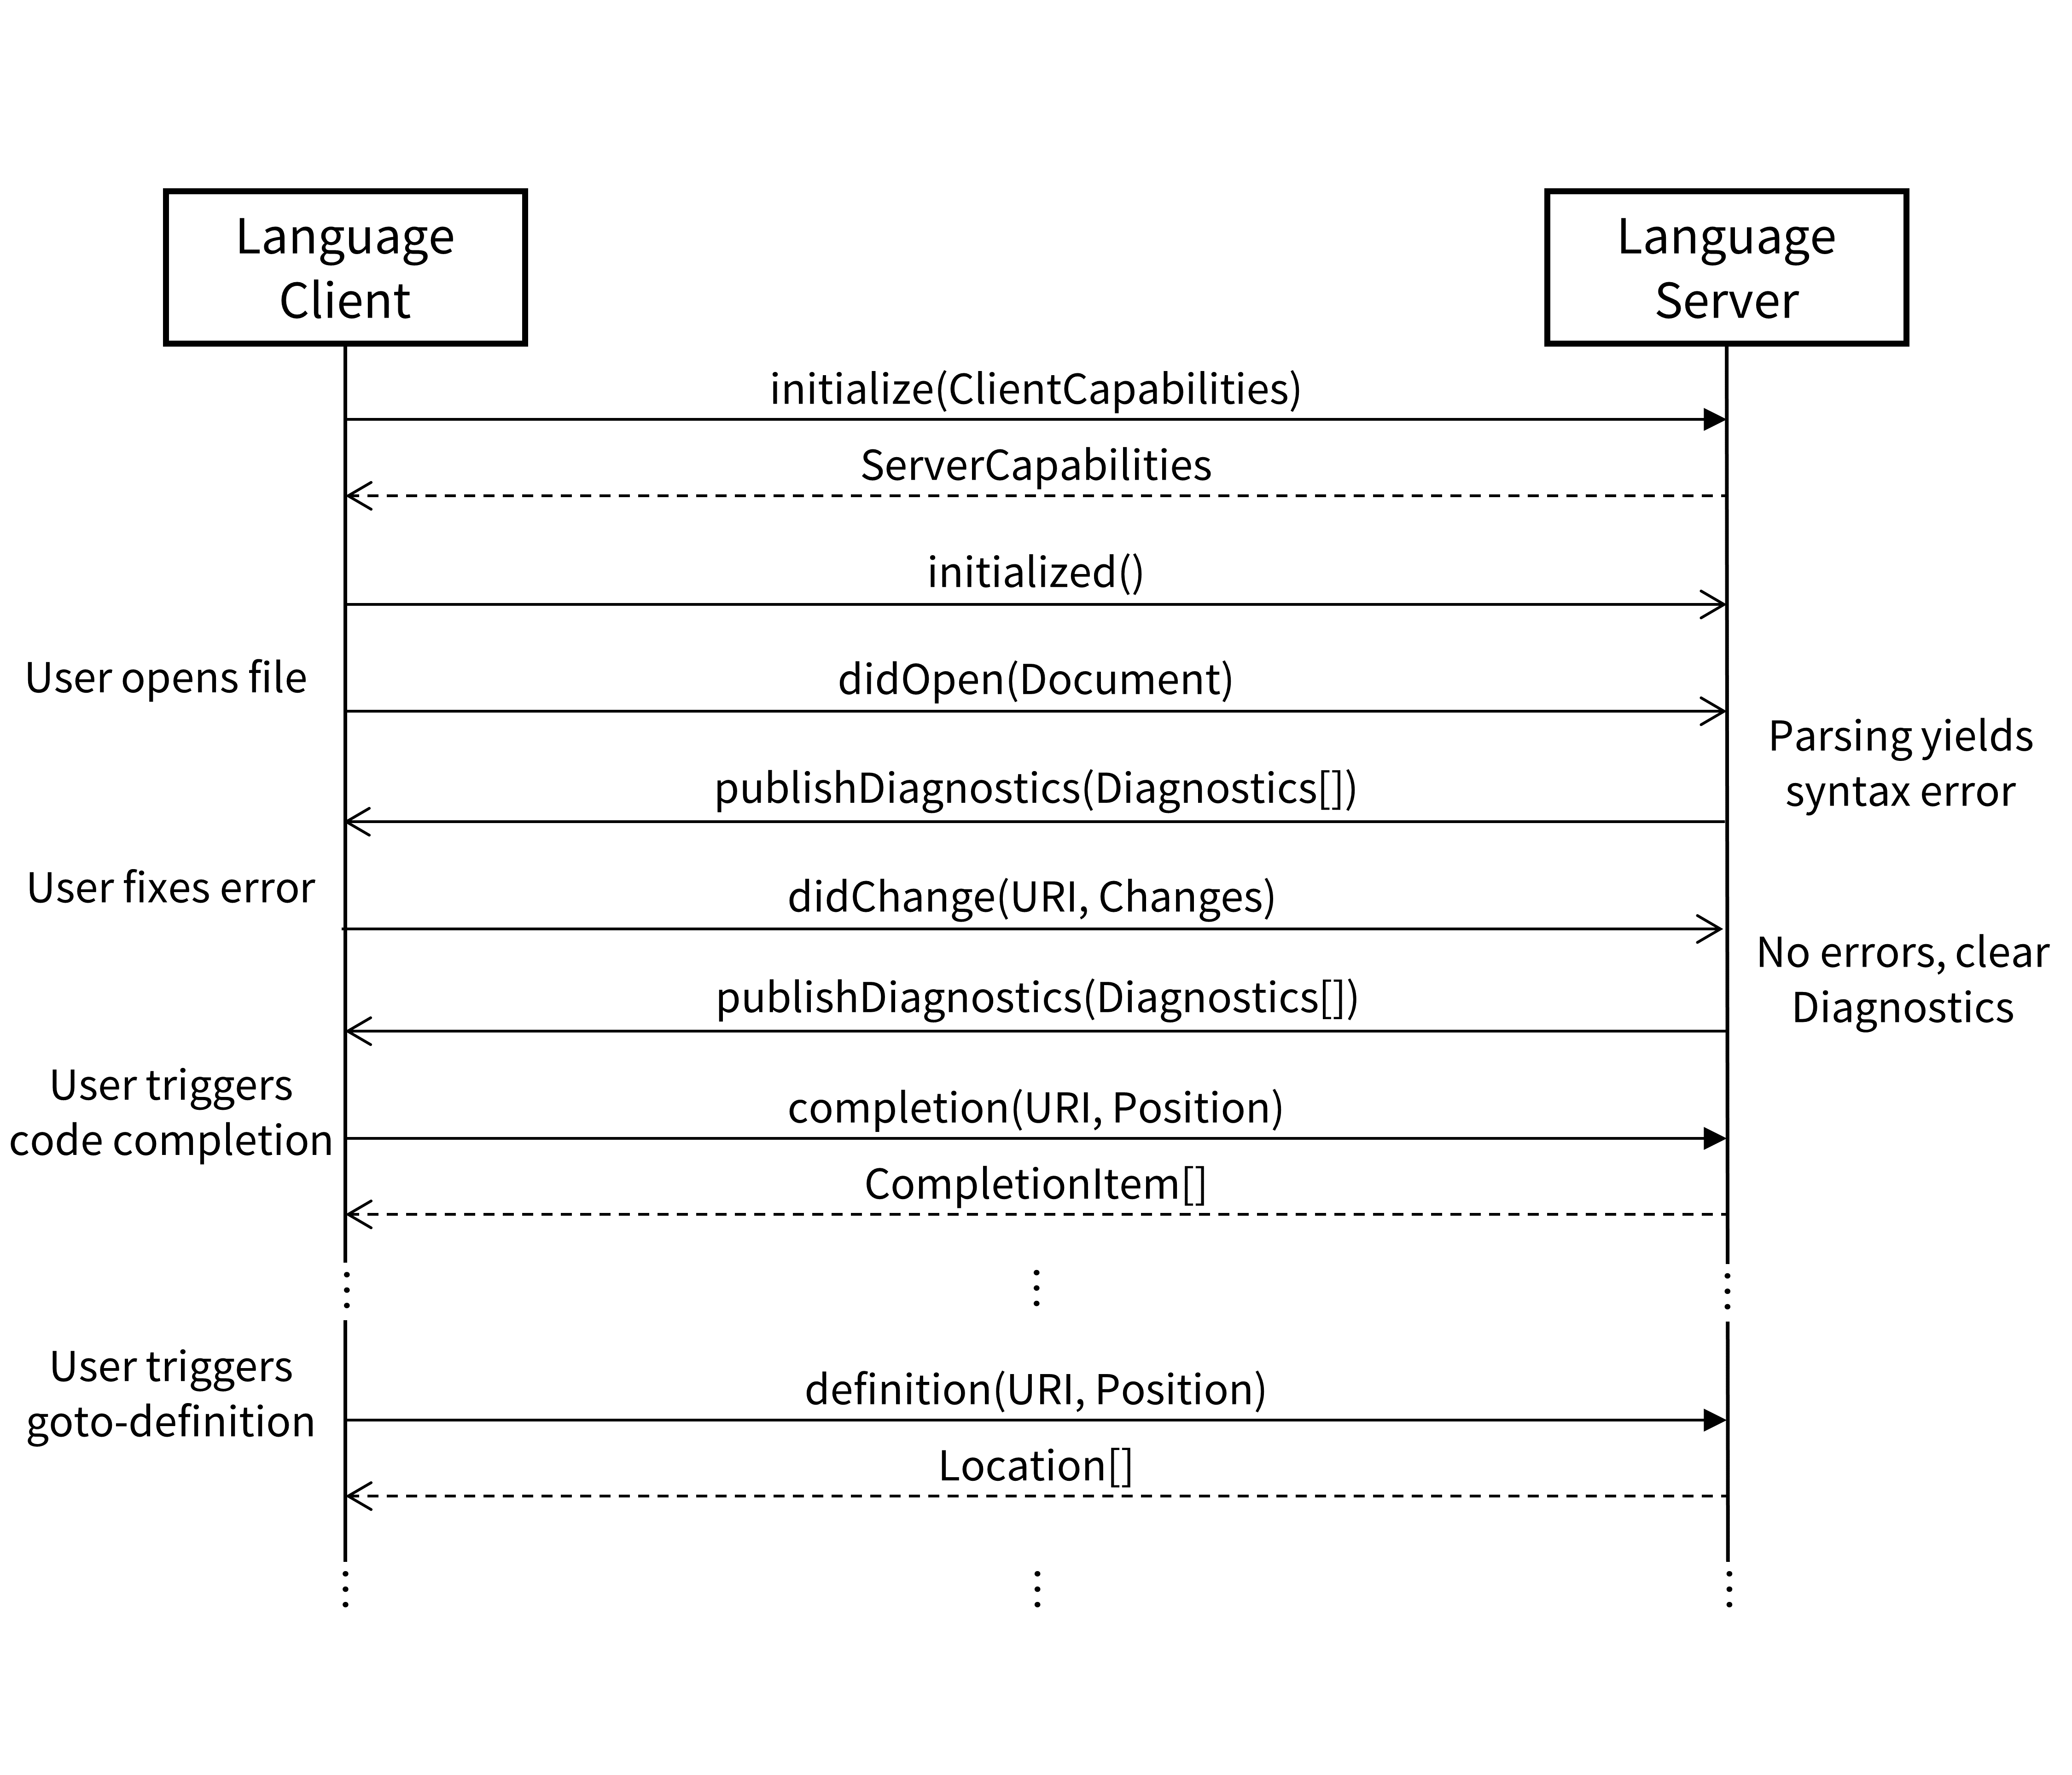
\includegraphics[width=\linewidth]{images/language-server-sequence_2.png}
%DIFDELCMD <   %%%
%DIFDELCMD < \caption[Exemplary communication between language client and server]{%
{%DIFAUXCMD
\DIFdelFL{An exemplary communication of language client and server, including initialization, opening and changing a file, and requesting a code completion and goto-definition.}}
  %DIFAUXCMD
%DIFDELCMD < \label{fig:lspsequence}
%DIFDELCMD < \end{figure}
%DIFDELCMD <     

%DIFDELCMD < \autoref{fig:lspsequence} %%%
\DIFdel{shows an exemplary communication between server and
client. After initialization, the client notifies the server that a file has
been opened. The server parses the source code, detects a syntax error and sends
this information to the client. The user fixes the displayed syntax error and
the client sends these changes incrementally to the server. After parsing again
on the server side, no errors occur, but the server needs to explicitly notify
the client about that, so that the client can clear the currently displaying
diagnostics. Then, the client sends a request for code completion at a specific
source location, typically the caret position. The server obtains completion
items depending on the provided context, which might also contain the trigger
character, and sends the items to the client. Later, a request to find one or
more definitions for a symbol at a position in the source code is sent to the
server. The server responds with a list of locations, if found.
}%DIFDELCMD < 

%DIFDELCMD < %%%
%DIF <  Typically, code editors like
%DIF <  Vim\footnote{\url{https://www.vim.org} (accessed 2018-12-17)}, Sublime
%DIF <  Text\footnote{\url{https://www.sublimetext.com} (accessed 2018-12-17)},
%DIF <  Atom\footnote{\url{https://atom.io} (accessed 2018-12-17)}, or Visual Studio
%DIF <  Code\footnote{\url{https://code.visualstudio.com} (accessed 2018-12-17)}, focus
%DIF <  on editing file-based programming or scripting languages. In addition to the
%DIF <  actual text editor view, modern graphical code editors also consist of a file
%DIF <  explorer, graphical debugger interface, and/or build-tools integration, which
%DIF <  are often made available as optional extensions for a variety of
%DIF <  languages. Popular \acp{ide} like
%DIF <  Eclipse\footnote{\url{https://www.eclipse.org/ide} (accessed 2018-12-17)},
%DIF <  Visual Studio\footnote{\url{https://visualstudio.microsoft.com} (accessed
%DIF <    2018-12-17)}, or IntelliJ\footnote{\url{https://www.jetbrains.com/idea}
%DIF <    (accessed 2018-12-17)} also have a code editor view as main component, but
%DIF <  focus on a richer support of one specific language by providing tailor-made,
%DIF <  integrated tools.  In the following, we will describe selected features of
%DIF <  source code editors, which are covered by the \ac{lsp} described in
%DIF <  \autoref{sec:lspcontext}.
%DIFDELCMD < 

%DIFDELCMD < %%%
\DIFdel{In this work we want to focus on some of the high-level features the \mbox{%DIFAUXCMD
\ac{lsp}
}\hspace{0pt}%DIFAUXCMD
supports and that most editors afford to their users:
}%DIFDELCMD < 

%DIFDELCMD < %%%
\paragraph{\DIFdel{Navigational Features}}
%DIFAUXCMD
\addtocounter{paragraph}{-1}%DIFAUXCMD
\DIFdel{These are the features code editors provide to navigate through source code. In
addition to pure textual searches, there might be a hierarchical outline views
or actions to find all definitions or references of a symbol.
}%DIFDELCMD < 

%DIFDELCMD < %%%
\paragraph{\DIFdel{Informational Features}}
%DIFAUXCMD
\addtocounter{paragraph}{-1}%DIFAUXCMD
\DIFdel{These features visualize source code related information, e.g. to display
signature and documentation, type information, or highlight uses of a symbol in
the same compilation unit. If a language parser detects syntax errors or a
linter provides some warnings, this information is also displayed in the code
editor.
}%DIFDELCMD < 

%DIFDELCMD < %%%
\paragraph{\DIFdel{Code-modifying Features}}
%DIFAUXCMD
\addtocounter{paragraph}{-1}%DIFAUXCMD
\DIFdel{This includes actions to format the whole file or a code snippet according to
some formatting rules as well as refactoring support. (Renaming of a symbol in
the current file or all files in the workspace is a simple example.) Sophisticated refactoring tools, however, are rather found in \mbox{%DIFAUXCMD
\acp{ide} }\hspace{0pt}%DIFAUXCMD
than
source code editors.
}%DIFDELCMD < 

%DIFDELCMD < %%%
\paragraph{\DIFdel{Code Completion}}
%DIFAUXCMD
\addtocounter{paragraph}{-1}%DIFAUXCMD
\DIFdel{Code completion is an important feature and typically integrated seamlessly into
the textual editor. We describe this feature in more detail here, because we will use it as a running example in }%DIFDELCMD < \autoref{cha:solution}%%%
\DIFdel{.
}%DIFDELCMD < 

%DIFDELCMD < %%%
\DIFdel{Code completion when triggered after object navigation characters (i.e. the
}\emph{\DIFdel{dot}} %DIFAUXCMD
\DIFdel{in Java) includes names of the methods and fields declared by the
object's type and super types before the navigation character. This kind of code
completion we call }%DIFDELCMD < \completionOfProperties%%%
\DIFdel{. For non-object-oriented languages,
}%DIFDELCMD < \completionOfProperties%%%
\DIFdel{~might not be supported or be limited to special language
elements, which understand some kind of }\emph{\DIFdel{property}}
%DIFAUXCMD
\DIFdel{semantic. }%DIFDELCMD < \CompletionOfProperties%%%
\DIFdel{~is often a challenge for languages with
untyped symbols}\DIFdelend \DIFaddbegin \DIFadd{instances of performance-focused language
implementation frameworks, and b) the \mbox{%DIFAUXCMD
\acf{lsp} }\hspace{0pt}%DIFAUXCMD
and how we approached supporting
it in a language-independent manner}\DIFaddend .

\DIFdelbegin \DIFdel{Another kind of code completion we will call }%DIFDELCMD < \completionOfGlobaslAndLocals%%%
\DIFdel{. In this case, the completion items depend on the surrounding scope rather than the
symbol in front of the cursor. With }\emph{\DIFdel{globals}} %DIFAUXCMD
\DIFdel{we refer to all the symbols
which we can derive from global scopes of languages. With }\emph{\DIFdel{locals}} %DIFAUXCMD
\DIFdel{we
analogously refer to all symbols which we can derive from local scopes of
languages. %DIF <  In the Python programming language for example, globals are built-in
%DIF <  functions or built-in classes. Locals of a function scope are function
%DIF <  parameters or local variables. \CompletionOfGlobaslAndLocals~might also be
%DIF <  triggered automatically, when the user starts typing a symbol, so that matching
%DIF <  globals and locals are suggested.
}%DIFDELCMD < 

%DIFDELCMD < %%%
\DIFdel{Because code completion is a core feature and is frequently auto-activated while
typing, Asaduzzaman has collected requirements of code completion systems
\mbox{%DIFAUXCMD
\cite{asaduzzaman2018context}}\hspace{0pt}%DIFAUXCMD
. Most of them address the fact, that the
completion system should not interrupt the user's flow of code writing.
}%DIFDELCMD < 

%DIFDELCMD < %%%
%DIF <  \subsection{Language Server Protocol}
%DIF <  \label{sec:lspcontext}
%DIFDELCMD < 

%DIFDELCMD < %%%
%DIF <  \paragraph{LSP4J}
%DIF <  Our implementation of \graallsp~uses
%DIF <  LSP4J\footnote{\url{https://github.com/eclipse/lsp4j}, version 0.4.1 (accessed
%DIF <    2018-12-17)} as Java binding for the \acl{lsp}. This framework maps the
%DIF <  \ac{lsp} requests and notifications to methods of Java interfaces so that
%DIF <  language server implementers do not have to deal with the \acs{json}-\acs{rpc}
%DIF <  communication layer and can make use of Java's type system.
%DIFDELCMD < 

%DIFDELCMD < %%%
%DIF <  \paragraph{Visual Studio Code}\todo{Is this important? Eventuell auf lang clients allgemein eingehen?}
%DIF <  We used Microsoft's source code editor Visual Studio Code\footnote{\url{https://code.visualstudio.com} (accessed 2018-12-17)} to create an exemplary language client extension and experiment with \graallsp.
%DIFDELCMD < 

%DIFDELCMD < %%%
%DIF <  \subsection{Terms and Concepts}
%DIF <      \paragraph{\acf{ast}}
%DIF <      Parsers for programming languages usually transform plain text source code into an \ac{ir} which can be processed by compilers, interpreters, or programming environment tools. An \ac{ast} is such a typical representation which stores structural information of the source code implicitly in its tree structure. Therefore, concrete syntactic elements needed to write parsable code in plain text can be omitted. In general, inner nodes of the \ac{ast} represent programming language operations and leaf nodes store the values needed for these operations. Depending on the use case, an \ac{ast} can store additional information in its nodes. For example the lexical source section from which a node was derived. Programming environment tools can use this information to display any kind of errors, warnings or hints directly in the plain text source code. An \ac{ast} interpreter evaluates an \ac{ast} by traversing its tree structure and executing the operations defined in the nodes.
%DIFDELCMD < 

%DIFDELCMD < %%%
%DIF <      \paragraph{Scopes and Frames}
%DIF <      A scope defines a region of a program in which a set of name bindings is valid, e.g. a local variable name.
%DIF <      Most programming languages have a concept of a global (program wide) scope and local scopes.
%DIF <      In a lexically scoped language, these local scopes can be obtained at compile-time and are for example defined by the nesting of modules, functions or blocks in the source code. In a dynamically scoped language, these local scopes depend on the call stack, i.e. the nesting of function calls. Today, most programming languages are lexically scoped.
%DIF <      At run-time, frames store the actual values of the name bindings of visible scopes.
%DIFDELCMD < 

%DIFDELCMD < %%%
\subsection[]{\DIFdel{Language Implementation Frameworks}}
%DIFAUXCMD
\addtocounter{subsection}{-1}%DIFAUXCMD
%DIFDELCMD < 

%DIFDELCMD < %%%
\DIFdel{Language Implementation Frameworks help a language developer in the process of
creating a new language. The feature set varies immensely, depending on the
purpose of the framework. Language workbenches like Spoofax
\mbox{%DIFAUXCMD
\cite{kats2010spoofax}}\hspace{0pt}%DIFAUXCMD
, Xtext \mbox{%DIFAUXCMD
\cite{eysholdt2010xtext}}\hspace{0pt}%DIFAUXCMD
, or MPS
\mbox{%DIFAUXCMD
\cite{voelter2012language}}\hspace{0pt}%DIFAUXCMD
, are used to develop and compose \mbox{%DIFAUXCMD
\acp{dsl} }\hspace{0pt}%DIFAUXCMD
together
with a corresponding \mbox{%DIFAUXCMD
\ac{ide} }\hspace{0pt}%DIFAUXCMD
with minimal effort, but their focus is not on
general purpose languages with good performance.
}%DIFDELCMD < 

%DIFDELCMD < %%%
\DIFdel{The kinds of frameworks }\DIFdelend \DIFaddbegin \subsection[]{\DIFadd{Tools in Language Implementation Frameworks}}

\DIFadd{In this work }\DIFaddend we are interested in \DIFdelbegin \DIFdel{in this work are
}\DIFdelend performance-focused \DIFaddbegin \DIFadd{language implementation
}\DIFaddend frameworks like Truffle~\cite{wimmer2012truffle} or RPython
\cite{ancona2007rpython}. In these frameworks, tooling has been a focus only
where it did not compete with performance\DIFdelbegin \DIFdel{, and thus }\DIFdelend \DIFaddbegin \DIFadd{. Thus, }\DIFaddend languages developed in these
frameworks have fewer tools available when compared to language workbenches \DIFaddbegin \DIFadd{like
Spoofax \mbox{%DIFAUXCMD
\cite{kats2010spoofax}}\hspace{0pt}%DIFAUXCMD
, Xtext \mbox{%DIFAUXCMD
\cite{eysholdt2010xtext}}\hspace{0pt}%DIFAUXCMD
, or MPS
\mbox{%DIFAUXCMD
\cite{voelter2012language}}\hspace{0pt}%DIFAUXCMD
, which are used to create \mbox{%DIFAUXCMD
\acp{dsl} }\hspace{0pt}%DIFAUXCMD
and their
corresponding \mbox{%DIFAUXCMD
\acp{ide}}\hspace{0pt}%DIFAUXCMD
}\DIFaddend .

\DIFdelbegin \paragraph{\DIFdel{Truffle and GraalVM}}
%DIFAUXCMD
\addtocounter{paragraph}{-1}%DIFAUXCMD
\DIFdelend %DIF >  \paragraph{Truffle and GraalVM}
Truffle~\cite{wimmer2012truffle} is a language implementation framework written
in Java. The language developer uses the framework to write an \ac{ast}
interpreter, which \DIFdelbegin \DIFdel{is able to optimize itself }\DIFdelend \DIFaddbegin \DIFadd{the framework optimizes }\DIFaddend during interpretation. \DIFdelbegin \DIFdel{To achieve
that, Truffle uses run-time type information to rewrite \mbox{%DIFAUXCMD
\ac{ast} }\hspace{0pt}%DIFAUXCMD
nodes. }\DIFdelend How source
code \DIFdelbegin \DIFdel{is }\DIFdelend parsed and the \ac{ast} is structured is the responsibility of the language
implementation. \DIFdelbegin %DIFDELCMD < 

%DIFDELCMD < %%%
\DIFdelend Truffle has built-in support for developing language-agnostic
tools by providing an instrumentation \DIFdelbegin \DIFdel{\mbox{%DIFAUXCMD
\ac{api}}\hspace{0pt}%DIFAUXCMD
~\mbox{%DIFAUXCMD
\cite{van2015building} }\hspace{0pt}%DIFAUXCMD
and a
system of tags and
source information }\DIFdelend \DIFaddbegin \api\DIFadd{~\mbox{%DIFAUXCMD
\cite{van2015building} }\hspace{0pt}%DIFAUXCMD
using a
meta-information }\DIFaddend that language implementations can attach to their \ac{ast}
nodes. \DIFdelbegin \DIFdel{It is designed to work well with the optimization techniques for language
implementations so that instrumentation can be done with nearly
zero-overhead. The framework can notify tools when a new source is loaded, a
statement is going to be executed, or an expression will return a value. The
focus of this instrumentation has been to build run-time tools like debuggers
and profilers.
}%DIFDELCMD < 

%DIFDELCMD < %%%
\DIFdel{To get high-performance language implementations, Truffle uses the
language-independent just-in-time compiler named
Graal~\mbox{%DIFAUXCMD
\cite{wurthinger2013one}}\hspace{0pt}%DIFAUXCMD
. Among other optimizations, Graal applies partial
evaluation to compile stable \mbox{%DIFAUXCMD
\ac{ast} }\hspace{0pt}%DIFAUXCMD
subtrees into optimized machine
code ~\mbox{%DIFAUXCMD
\cite{wurthinger2017practical}}\hspace{0pt}%DIFAUXCMD
. These optimizations do not stop at language
boundaries, so that the access of foreign language objects can also be
optimized}\DIFdelend \DIFaddbegin \DIFadd{This }\api \DIFadd{has been used already to provide all Truffle languages
with code coverage, CPU and memory profiling tools, as well as debugging with
the Chrome debugger protocol that's also supported by the VSCode, IntelliJ, and
Netbeans}\DIFaddend .

\DIFdelbegin %DIFDELCMD < \begin{figure}
%DIFDELCMD <   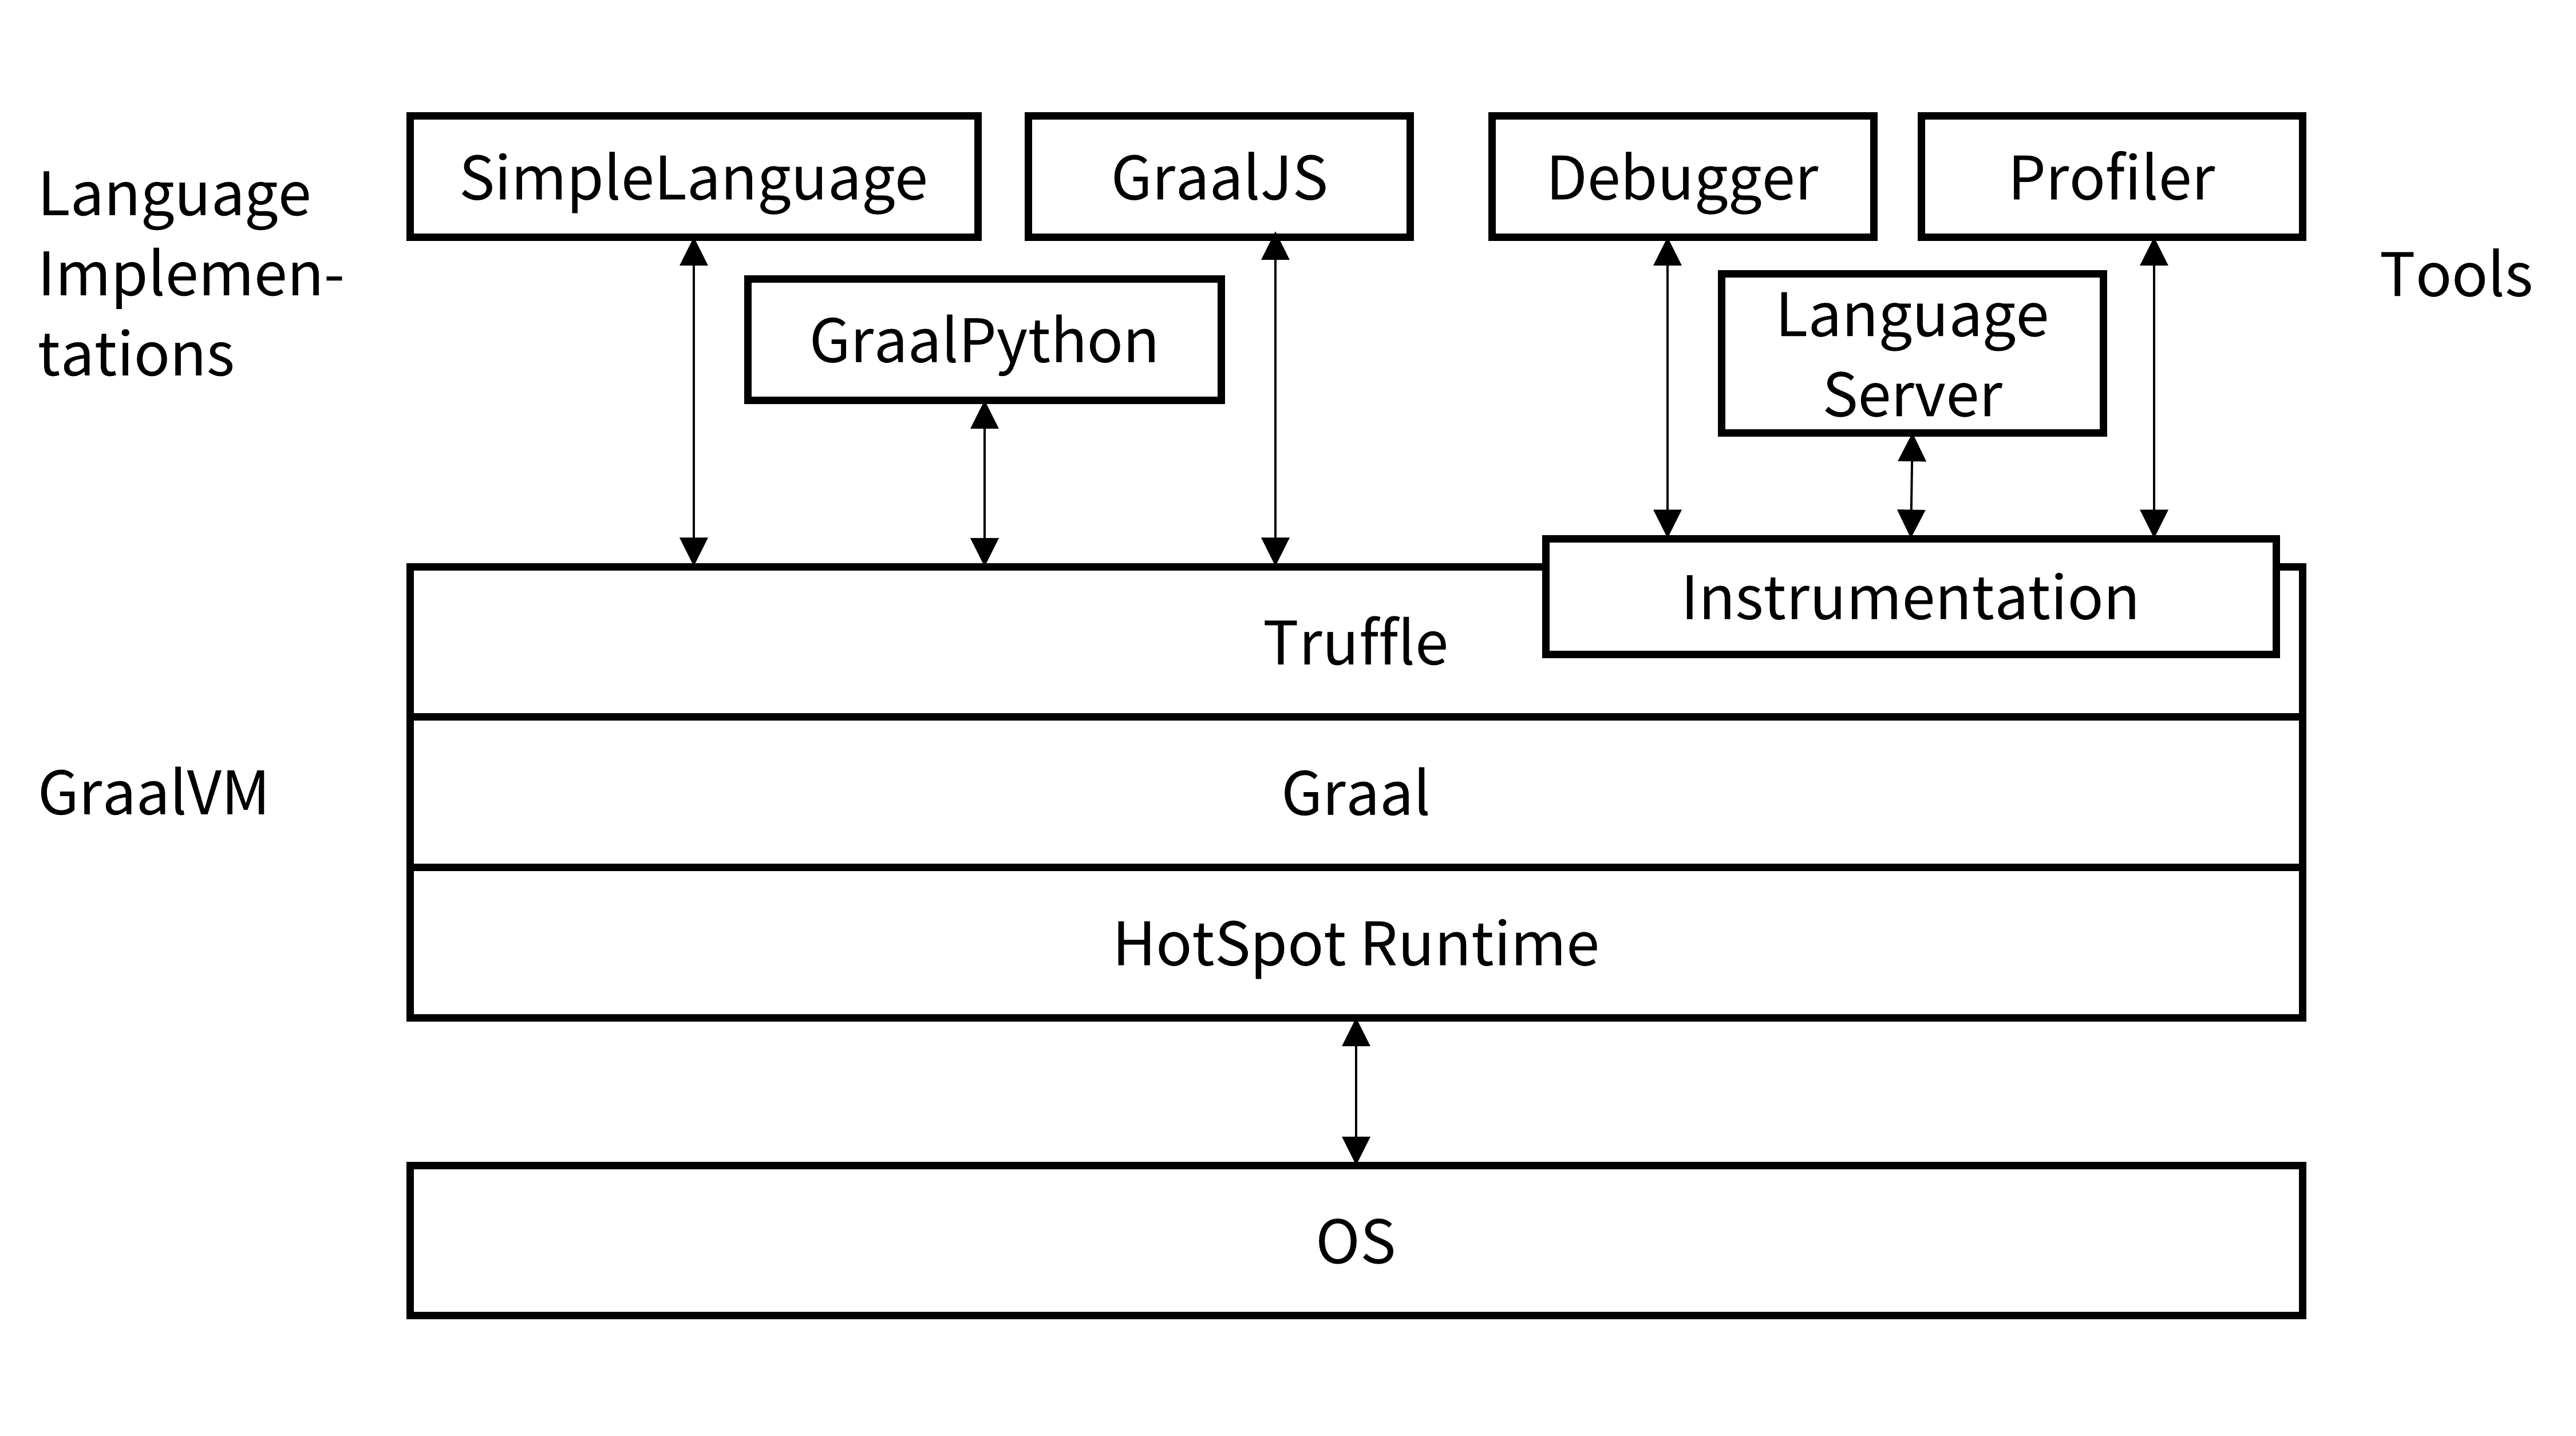
\includegraphics[width=\linewidth]{images/GraalVM-Truffle-stack_1.png}
%DIFDELCMD <   %%%
%DIFDELCMD < \caption[Architecture stack of the GraalVM]{%
{%DIFAUXCMD
\DIFdelFL{Truffle languages and tools hosted by the Truffle framework on top of the GraalVM.}}
  %DIFAUXCMD
%DIFDELCMD < \label{fig:graaltrufflestack}
%DIFDELCMD < \end{figure}
%DIFDELCMD <     

%DIFDELCMD < %%%
%DIF <  \subsubsection{GraalVM}
%DIF <      GraalVM\cite{graalvm2018} is a high-performance polyglot VM.
%DIF <      Graal/Truffle: Performance first \cite{grimmer2015high}. 
%DIFDELCMD < 

%DIFDELCMD < %%%
%DIF <      %https://www.graalvm.org/
%DIF <      GraalVM is a universal virtual machine for running applications written in JavaScript, Python 3, Ruby, R, JVM-based languages like Java, Scala, Kotlin, and LLVM-based languages such as C and C++.
%DIFDELCMD < 

%DIFDELCMD < %%%
%DIF <      GraalVM removes the isolation between programming languages and enables interoperability in a shared runtime. It can run either standalone or in the context of OpenJDK, Node.js, Oracle Database, or MySQL.
%DIF <      %https://www.graalvm.org/
%DIFDELCMD < 

%DIFDELCMD < %%%
%DIF <      % https://medium.com/graalvm/graalvm-ten-things-12d9111f307d
%DIF <      You can use Truffle to implement your own new programming language, to create a high-performance implementation of an existing programming language, or to implement a domain specific language. We talk a lot about the details of Truffle and Graal in our project, but we often forget to mention that Truffle is the easy way to implement a language. And you get features like the debugger automatically. Anyone who’s done just an undergraduate course in programming language implementation should have the basic skills needed. Oracle Labs implemented a basic version of Ruby faster than any previous efforts with just one intern over a few months.
%DIF <      % https://medium.com/graalvm/graalvm-ten-things-12d9111f307d
%DIFDELCMD < 

%DIFDELCMD < %%%
%DIF <      \subsubsection{Instrumentation}
%DIF <      % https://www.graalvm.org/docs/graalvm-as-a-platform/
%DIF <      Implement your own Tools
%DIFDELCMD < 

%DIFDELCMD < %%%
%DIF <      GraalVM provides a framework for creating language-agnostic tools like debuggers, profilers, or other instrumentations. In general, GraalVM provides a standardized way to express and run program code enabling cross-language research and the development of tools that are developed once and then can be applied to any language.
%DIF <      % https://www.graalvm.org/docs/graalvm-as-a-platform/
%DIFDELCMD < 

%DIFDELCMD < %%%
%DIF <      % https://www.graalvm.org/docs/why-graal/
%DIF <      Create Language-agnostic Tools
%DIFDELCMD < 

%DIFDELCMD < %%%
%DIF <      GraalVM provides a framework for creating language-agnostic tools like debuggers, profilers, or other instrumentations. GraalVM provides a standardized way to express and run program code enabling cross-language research and the development of tools that are developed once and then can be applied to any language.
%DIF <      % https://www.graalvm.org/docs/why-graal/
    %DIFDELCMD < 

%DIFDELCMD < %%%
\paragraph{\DIFdel{PyPy and RPython}}
    %DIFAUXCMD
\addtocounter{paragraph}{-1}%DIFAUXCMD
%DIF <  \begin{itemize}
    %DIF <      \item bytecode interpreter
    %DIF <      \item type inference \cite{maia2012static}
    %DIF <      \item http://stefan-marr.de/papers/oopsla-marr-ducasse-meta-tracing-vs-partial-evaluation/
    %DIF <  \end{itemize}
%DIFDELCMD < 

%DIFDELCMD < %%%
\DIFdelend PyPy \cite{rigo2006pypy} is an alternative implementation of the Python
\cite{Rossum1995} language \DIFdelbegin \DIFdel{. It uses a tracing \mbox{%DIFAUXCMD
\ac{jit} }\hspace{0pt}%DIFAUXCMD
compiler
\mbox{%DIFAUXCMD
\cite{bolz2009tracing} }\hspace{0pt}%DIFAUXCMD
so that many Python programs can be executed faster than
using the default \mbox{%DIFAUXCMD
\ac{vm} }\hspace{0pt}%DIFAUXCMD
implementation }\emph{\DIFdel{CPython}}%DIFAUXCMD
\DIFdel{.
}%DIFDELCMD < 

%DIFDELCMD < %%%
\DIFdel{RPython\mbox{%DIFAUXCMD
\cite{ancona2007rpython} }\hspace{0pt}%DIFAUXCMD
is a translation and support framework for
developing dynamic programming languages. The RPython language is }\DIFdelend \DIFaddbegin \DIFadd{written using RPython, }\DIFaddend a restricted subset of \DIFdelbegin \DIFdel{Python. It disallows some of the
dynamic features of Python to apply
static analysis. Thus, source code written in RPython can be translated to C by
deriving low-level C types from Python data types. Language implementers use the framework to write a bytecode interpreter with hints for the RPython tool chain, so that the interpreter can be optimized by PyPy's tracing \mbox{%DIFAUXCMD
\ac{jit} }\hspace{0pt}%DIFAUXCMD
compiler. }%DIFDELCMD < 

%DIFDELCMD < %%%
\DIFdelend \DIFaddbegin \DIFadd{the
Python language. The language developer is free to structure the interpreter as
they see fit, although bytecode interpreters are the most common approach for
RPython-based languages. %DIF >  It uses a tracing \ac{jit} compiler
%DIF >  \cite{bolz2009tracing} so that many Python programs can be executed faster
%DIF >  than using the default \ac{vm} implementation \emph{CPython}.  RPython
%DIF >  \cite{ancona2007rpython} is a translation and support framework for developing
%DIF >  dynamic programming languages. The RPython language is a restricted subset of
%DIF >  Python. It disallows some of the dynamic features of Python to apply static
%DIF >  analysis. Thus, source code written in RPython can be translated to C by
%DIF >  deriving low-level C types from Python data types. Language implementers use
%DIF >  the framework to write a bytecode interpreter with hints for the RPython tool
%DIF >  chain, so that the interpreter can be optimized by PyPy's tracing \ac{jit}
%DIF >  compiler.
}\DIFaddend RPython provides no \DIFdelbegin \DIFdel{explicit \mbox{%DIFAUXCMD
\ac{api} }\hspace{0pt}%DIFAUXCMD
for tools as described for the Truffle framework. The only notable example of a run-time tool is VMProf, a profiler to
understand and resolve performance bottlenecks. The language developer registers
}\DIFdelend \DIFaddbegin \DIFadd{generic }\api \DIFadd{for tools like Truffle does. However, the
RPython library includes a CPU profiler and a reverse debugger. Languages can
make use of these with minimal effort by registering }\DIFaddend entry points for the \DIFdelbegin \DIFdel{profiler by annotating functions }\DIFdelend with
certain Python decorators and by implementing \DIFdelbegin \DIFdel{a callback to get string representations of the guest language objects}\DIFdelend \DIFaddbegin \DIFadd{callbacks to attach for the tools
to call into}\DIFaddend .

\DIFdelbegin \section[]{\DIFdel{Approach}}
%DIFAUXCMD
\addtocounter{section}{-1}%DIFAUXCMD
%DIFDELCMD < \label{cha:solution}
%DIFDELCMD < 

%DIFDELCMD < %%%
%DIF <  \paragraph{Alternative approach outline}
%DIF <  \begin{itemize}
%DIF <      \item aim: map LSP requests to language implementation framework
%DIF <      \item assumption: language implementation framework has some kind of language-agnostic tooling API
%DIF <      \item rule: "use as much static infos as the framework provides - for all missing infos: observe execution to learn about the behavior of our code"
%DIF <      \item running example code completion: 1. parse code; 2. map cursor position to parsing result IR (AST); 3. Consider context; 4. Obtain completion items to build LSP response
%DIF <      \item Parsing code and mapping to IR
%DIF <          \begin{itemize}
%DIF <              \item parsing: didOpen / didChange (handle incremental code changes)
%DIF <              \item errors: diagnostics notification (can parser handle multiple errors? or fail-at-first-error?)
%DIF <              \item mapping: line+column -> IR (e.g. AST node)
%DIF <          \end{itemize}
%DIF <      \item static info exploitation
%DIF <          \begin{itemize}
%DIF <              \item code completion: globals (built-ins) + locals via lexical scopes
%DIF <              \item (documentSymbol: use meta-infos of IR, e.g. tags of AST nodes in Truffle)
%DIF <              \item (...)
%DIF <          \end{itemize}
%DIF <      \item collecting dynamic infos
%DIF <          \begin{itemize}
%DIF <              \item exec code to collect run-time infos
%DIF <              \item requirements: instrumentation / tracing of host language
%DIF <              \item challenges
%DIF <                  \begin{itemize}
%DIF <                      \item side-effects -> sandboxing
%DIF <                      \item endless execution -> break exec on result + timeout
%DIF <                      \item caret position not reached -> run-script or unit tests
%DIF <                      \item unsaved changes -> custom file system
%DIF <                      \item performance -> caching + codeLense request for explicit cache refresh
%DIF <                  \end{itemize}
%DIF <              \item code completion: for locals use frame to get run-time scopes
%DIF <              \item code completion of properties: query run-time object for properties
%DIF <          \end{itemize}
%DIF <      \item transfer to other requests
%DIF <          \begin{itemize}
%DIF <              \item signatureHelp
%DIF <              \item hover
%DIF <              \item documentSymbol
%DIF <              \item symbol
%DIF <              \item definition
%DIF <              \item references
%DIF <              \item documentHighlight
%DIF <          \end{itemize}
%DIF <      \item further language-agnostic challenges
%DIF <          \begin{itemize}
%DIF <              \item initialize: need to name completion and signatureHelp trigger characters
%DIF <              \item completion and signatureHelp: check if request is triggered by trigger of this language
%DIF <          \end{itemize}
%DIF <  \end{itemize}
%DIFDELCMD < 

%DIFDELCMD < %%%
%DIF <  \clearpage
%DIFDELCMD < 

%DIFDELCMD < %%%
%DIF <  \paragraph{new apporach}
%DIF <  In \autoref{cha:introduction} we described the problem, that run-time
%DIF <  performance-focused language implementation frameworks lack \ac{ide}-like
%DIF <  tooling support for the developed languages. Therefore, we suggest to build a
%DIF <  language-agnostic language server on top of these kind of frameworks to start
%DIF <  closing the tooling gap. Because most of the currently implemented languages of
%DIF <  frameworks like RPython or Truffle are dynamic and the support of features like
%DIF <  code completion is especially difficult for these kind of languages, we focus on
%DIF <  dynamic and dynamically typed language implementations in our approach.
\DIFdelend \DIFaddbegin \subsection[]{\DIFadd{Code Editors and the Language Server Protocol}}
\label{sec:contextSourceCodeEditors}
\DIFaddend 

\DIFdelbegin \DIFdel{Typically, a language server is developed for one specific language only and the server implementation can exploit any kind of }\DIFdelend \DIFaddbegin \DIFadd{A huge number of code editors exist and the choice of editor is an amusingly
frequent source of arguments amongst
developers. The~\mbox{%DIFAUXCMD
\acf{lsp}}\hspace{0pt}%DIFAUXCMD
}\footnote{\url{https://microsoft.github.io/language-server-protocol}
  \DIFadd{(accessed 2018-12-17). At the date of writing, language servers for more than
  50 languages exist. Usually, these language server implementations support
  exactly one language, but the \mbox{%DIFAUXCMD
\ac{lsp} }\hspace{0pt}%DIFAUXCMD
allows multiple languages per server.}}
\DIFadd{is an approach to standardize language support for development tools to make the
choice of editor less tied to the choice of language. The \mbox{%DIFAUXCMD
\ac{lsp} }\hspace{0pt}%DIFAUXCMD
defines a
}\emph{\DIFadd{server}} \DIFadd{and a }\emph{\DIFadd{client}}\DIFadd{. The server needs to be implemented only once
for every language, providing the }\DIFaddend language-specific \DIFdelbegin \DIFdel{information. To
implement a language-agnostic language server, we have to build upon the
abstract concepts and \mbox{%DIFAUXCMD
\acp{api} }\hspace{0pt}%DIFAUXCMD
of language implementation frameworks, which
apply to all languages developed in these frameworks.  In the following, we use
the
example of code completion to describe our approach. First of all, we show
which kind of data is needed to respond to the }\emph{\DIFdel{completion}} %DIFAUXCMD
\DIFdel{request of \mbox{%DIFAUXCMD
\ac{lsp}}\hspace{0pt}%DIFAUXCMD
}\DIFdelend \DIFaddbegin \DIFadd{development features. Any
editor that can act as a language client can make use of any language server and
therefore support multiple languages with minimal effort}\DIFaddend .
\DIFdelbegin \DIFdel{Then, we suggest how languageimplementation frameworks can obtain the needed information in a language-agnostic way.
}%DIFDELCMD < 

%DIFDELCMD < %%%
\subsection[]{\DIFdel{Completion of Globals and Locals}}
%DIFAUXCMD
\addtocounter{subsection}{-1}%DIFAUXCMD
%DIFDELCMD < \label{sec:newApproach:completionOfGlobals}
%DIFDELCMD < %%%
\DIFdelend 

\DIFdelbegin \DIFdel{In }%DIFDELCMD < \autoref{sec:contextSourceCodeEditors} %%%
\DIFdel{we distinguished two kinds of code
completions. We start with the Python code snippet in
}%DIFDELCMD < \autoref{lst:pythonNearCaretExample1NewApproach} %%%
\DIFdel{to explain how to support code
completion of globals and
locals.
}\DIFdelend %DIF >  \paragraph{Client and Server Communication}
%DIF >  \ac{lsp} client and server communicate via
%DIF >  \acs{json}-\acs{rpc}\footnote{\url{https://www.jsonrpc.org/specification}
%DIF >    (accessed 2018-12-17)} requests, responses and notifications. Source code
%DIF >  files are referenced by \acp{uri}. A location in the source code is encoded as
%DIF >  line and column tuple. During initialization, client and server can exchange
%DIF >  which features are supported.

\DIFdelbegin %DIFDELCMD < \begin{code}[lst:pythonNearCaretExample1NewApproach]{Completions in Python code}{float,numbers=right,language=Python}
%DIFDELCMD < %%%
\DIFdel{def foo(param1, param2):
    x = 42
}\DIFdelend %DIF >  \begin{figure}
%DIF >    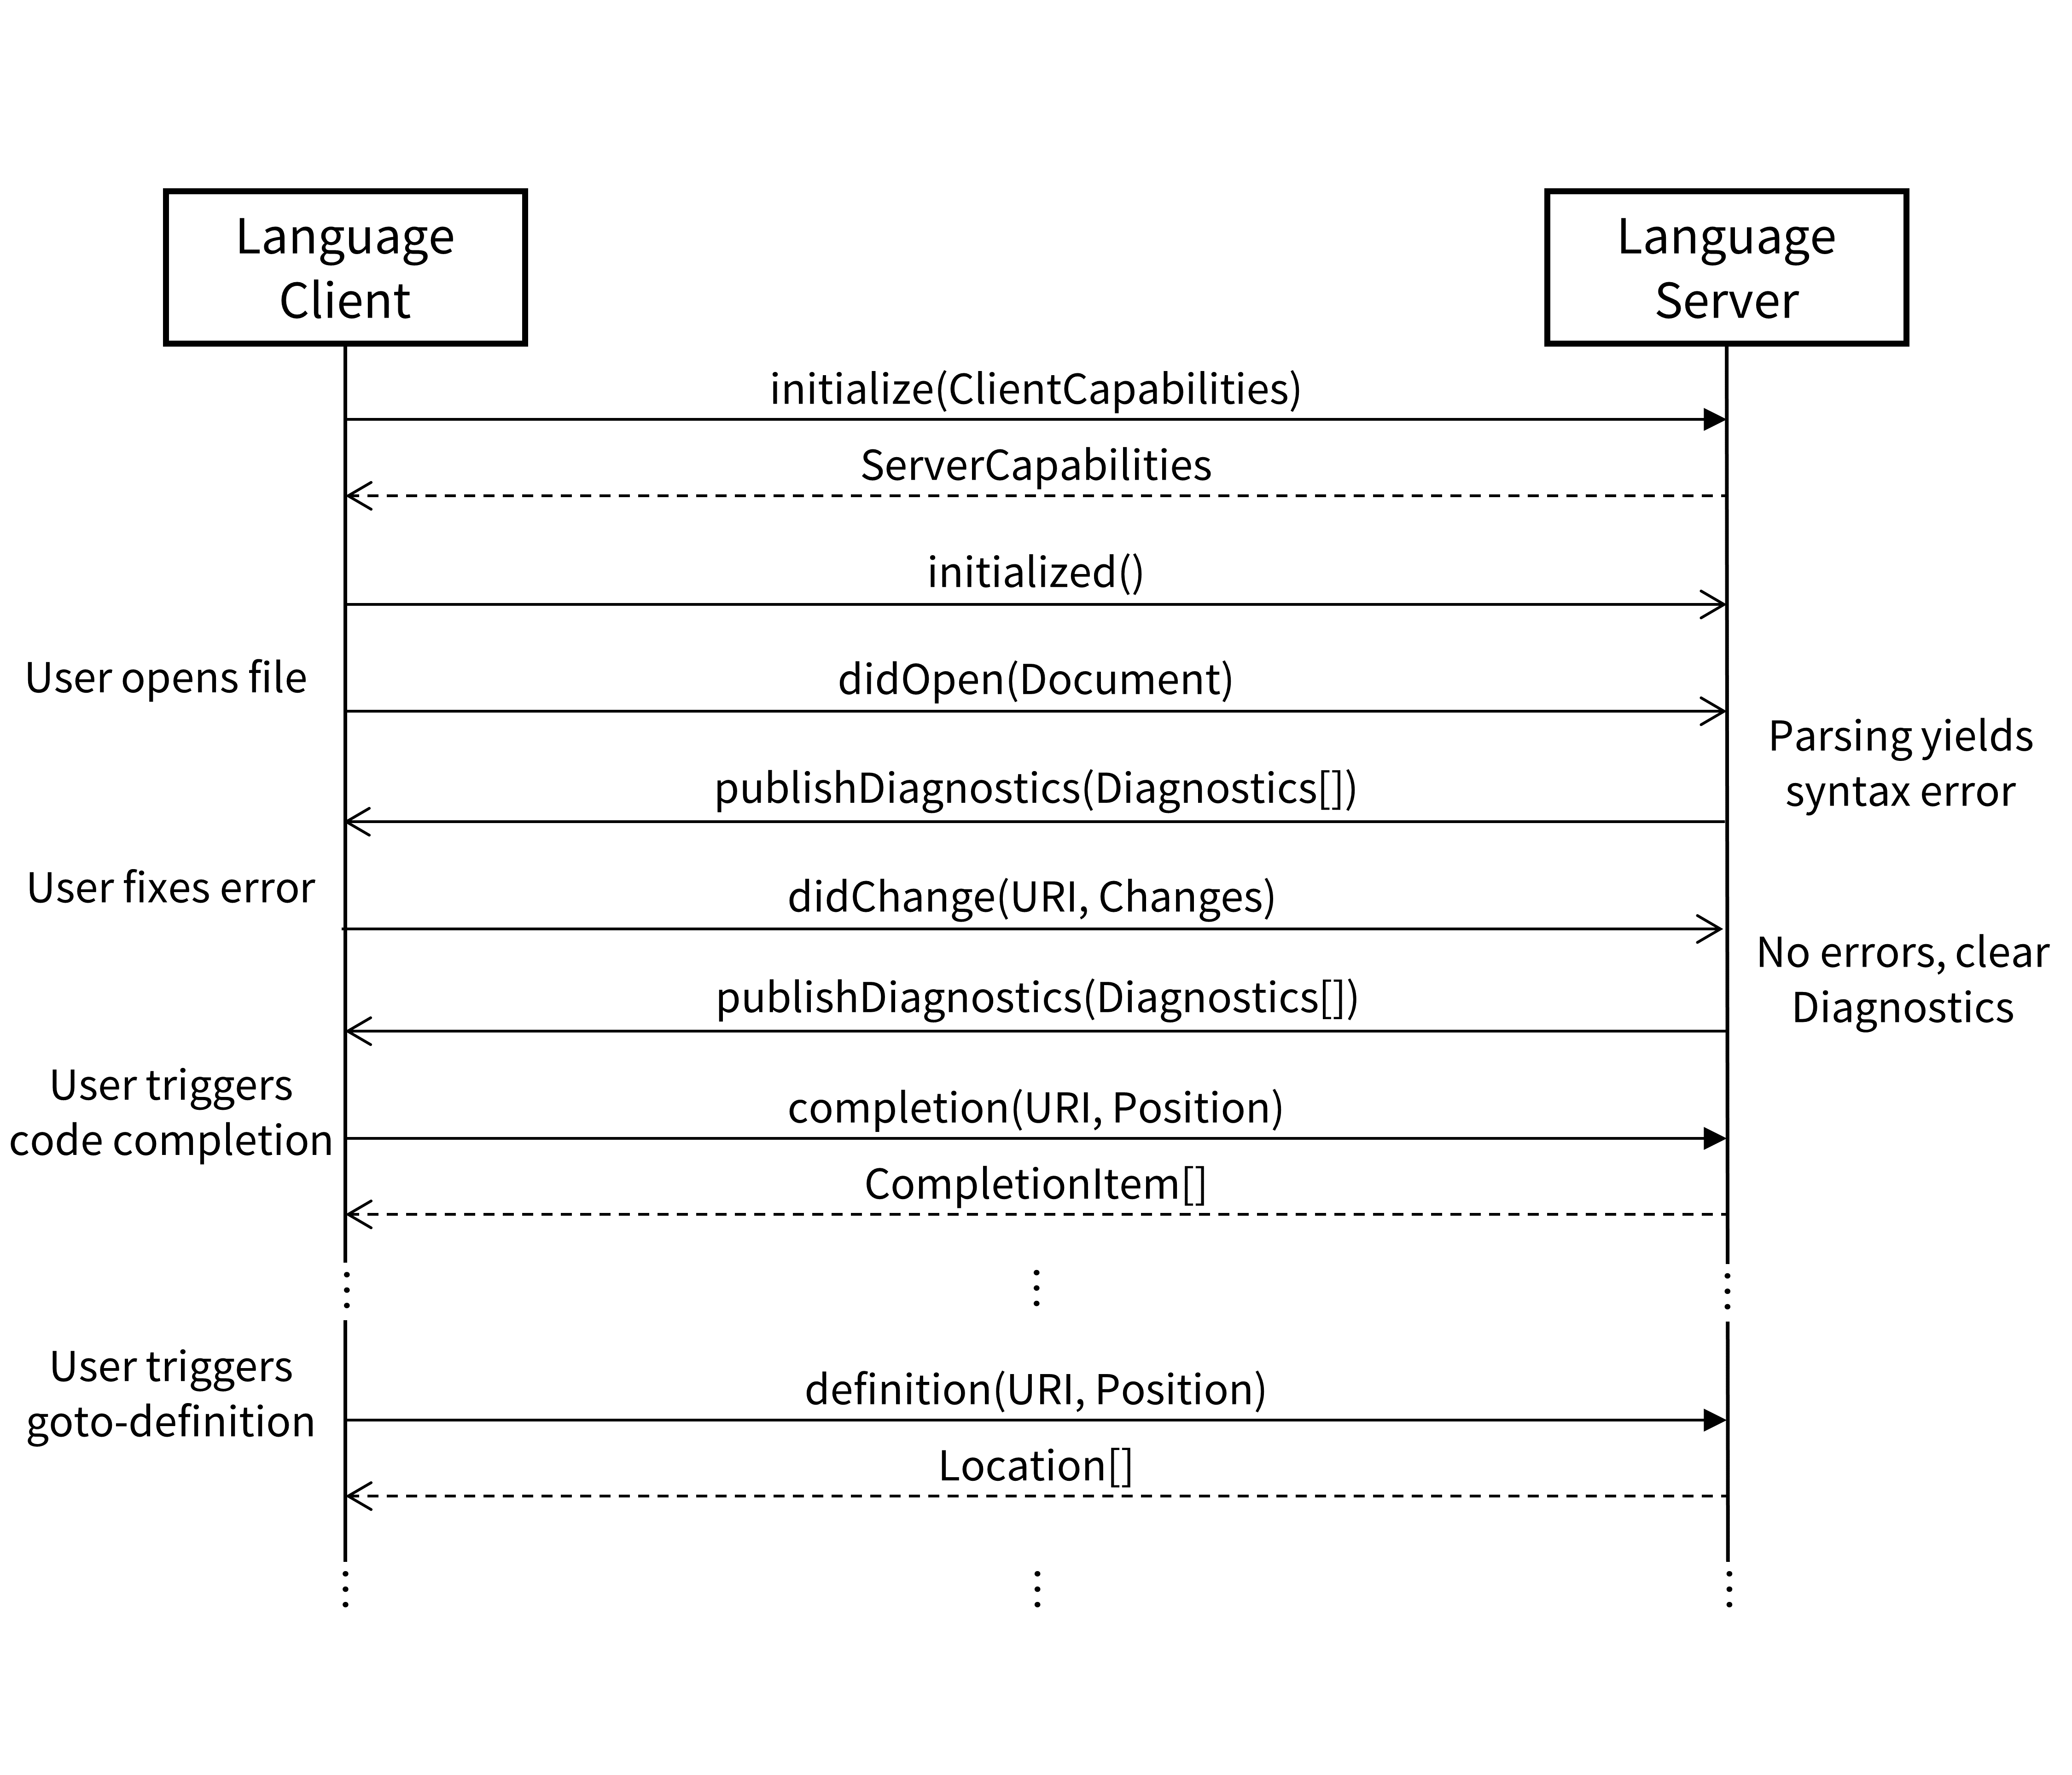
\includegraphics[width=\linewidth]{images/language-server-sequence_2.png}
%DIF >    \caption[Exemplary communication between language client and server]{An exemplary communication of language client and server, including initialization, opening and changing a file, and requesting a code completion and goto-definition.}
%DIF >    \label{fig:lspsequence}
%DIF >  \end{figure}

\DIFdelbegin \DIFdel{y = param1 + param2
}\DIFdelend %DIF >  \autoref{fig:lspsequence} shows an exemplary communication between server and
%DIF >  client. After initialization, the client notifies the server that a file has
%DIF >  been opened. The server parses the source code, detects a syntax error and sends
%DIF >  this information to the client. The user fixes the displayed syntax error and
%DIF >  the client sends these changes incrementally to the server. After parsing again
%DIF >  on the server side, no errors occur, but the server needs to explicitly notify
%DIF >  the client about that, so that the client can clear the currently displaying
%DIF >  diagnostics. Then, the client sends a request for code completion at a specific
%DIF >  source location, typically the caret position. The server obtains completion
%DIF >  items depending on the provided context, which might also contain the trigger
%DIF >  character, and sends the items to the client. Later, a request to find one or
%DIF >  more definitions for a symbol at a position in the source code is sent to the
%DIF >  server. The server responds with a list of locations, if found.

\DIFdelbegin \DIFdel{print(x * y)
}%DIFDELCMD < \end{code}
%DIFDELCMD < %%%
\DIFdelend %DIF >  Typically, code editors like
%DIF >  Vim\footnote{\url{https://www.vim.org} (accessed 2018-12-17)}, Sublime
%DIF >  Text\footnote{\url{https://www.sublimetext.com} (accessed 2018-12-17)},
%DIF >  Atom\footnote{\url{https://atom.io} (accessed 2018-12-17)}, or Visual Studio
%DIF >  Code\footnote{\url{https://code.visualstudio.com} (accessed 2018-12-17)}, focus
%DIF >  on editing file-based programming or scripting languages. In addition to the
%DIF >  actual text editor view, modern graphical code editors also consist of a file
%DIF >  explorer, graphical debugger interface, and/or build-tools integration, which
%DIF >  are often made available as optional extensions for a variety of
%DIF >  languages. Popular \acp{ide} like
%DIF >  Eclipse\footnote{\url{https://www.eclipse.org/ide} (accessed 2018-12-17)},
%DIF >  Visual Studio\footnote{\url{https://visualstudio.microsoft.com} (accessed
%DIF >    2018-12-17)}, or IntelliJ\footnote{\url{https://www.jetbrains.com/idea}
%DIF >    (accessed 2018-12-17)} also have a code editor view as main component, but
%DIF >  focus on a richer support of one specific language by providing tailor-made,
%DIF >  integrated tools.  In the following, we will describe selected features of
%DIF >  source code editors, which are covered by the \ac{lsp} described in
%DIF >  \autoref{sec:lspcontext}.

%DIF <  Imagine, the listed Python code snippet is the content of a file which was
%DIF <  opened in an \ac{lsp}-supporting source code editor and the language client
%DIF <  implementation has already reported the opening of the file using the
%DIF <  \emph{didOpen} notification to our language server. This notification includes
%DIF <  the content and the \ac{uri} of the file. Now, 
\DIFdelbegin \DIFdel{With the caret on line 3, a }\emph{\DIFdel{completion}} %DIFAUXCMD
\DIFdel{request is sent to the server for
line 3 at character offset 4. We would expect a completion result to include
items for all Python globals (e.g. built-in functions) and the locals
}%DIFDELCMD < \inlinecode{param1}%%%
\DIFdel{, }%DIFDELCMD < \inlinecode{param2}%%%
\DIFdel{, and }%DIFDELCMD < \inlinecode{x}%%%
\DIFdel{. The variable
}%DIFDELCMD < \inlinecode{y} %%%
\DIFdel{should not be included, because no value is assigned to
it until
line 4. Besides a display name, a \mbox{%DIFAUXCMD
\ac{lsp} }\hspace{0pt}%DIFAUXCMD
completion item can optionally
contain a completion kind (e.g. variable, function, or class), a detail text for
signature or type information, and a documentation. To provide these items, we
suggest the following steps. }\DIFdelend \DIFaddbegin \DIFadd{For a number of Truffle languages (including R, Python, Ruby, and JavaScript),
multiple \mbox{%DIFAUXCMD
\ac{lsp} }\hspace{0pt}%DIFAUXCMD
server implementations already exist and these can be used
with these implementations directly. However, both Truffle already tries to
obsolete the need for multiple implementations of a GC, JIT, dynamic object
model, debugger, profiler, and more. We argue that there should not be a need
for multiple implementations of language servers, either.
}\DIFaddend 

\DIFdelbegin %DIFDELCMD < \begin{enumerate}
%DIFDELCMD < %%%
\DIFdelend \DIFaddbegin \DIFadd{In this work we focus on how Truffle can (in a language independent manner)
support a subset of the features of the \mbox{%DIFAUXCMD
\ac{lsp}}\hspace{0pt}%DIFAUXCMD
:
}\begin{enumerate*}[label=\arabic*) ]%DIF > 
\DIFaddend \item \DIFdelbegin \DIFdel{Parse the source code into a language-agnostic \mbox{%DIFAUXCMD
\ac{ir} }\hspace{0pt}%DIFAUXCMD
of the
  framework. This just re-uses the parser that the language developer has to
  write anyway. This parser will typically be syntax-error intolerant, so that
  we can support code completion only if the source code is parsable.
}\DIFdelend \DIFaddbegin \DIFadd{navigational features to follow references of names and go to the
  implementations of functions;
%DIF >  \item renaming as an example of a code-modifying feature;
}\DIFaddend \item \DIFdelbegin \DIFdel{Map line and column of the completion request to the \mbox{%DIFAUXCMD
\ac{ir}}\hspace{0pt}%DIFAUXCMD
. To do this,
  we assume selected elements of the \mbox{%DIFAUXCMD
\ac{ir} }\hspace{0pt}%DIFAUXCMD
allow access lexical
  representations in the source code. This information allows us to search for
  an \mbox{%DIFAUXCMD
\ac{ir} }\hspace{0pt}%DIFAUXCMD
element which maps best to the position of the completion
  request. Which one that should be in particular depends on the \mbox{%DIFAUXCMD
\ac{ir} }\hspace{0pt}%DIFAUXCMD
and the
  framework. We therefore assume that language implementations can expose
  further meta-information in a language-agnostic way through the framework, so
  that we can determine relevant language elements, like read- and
  write-accesses to variables, calls to callable elements, or definitions.
}\DIFdelend \DIFaddbegin \DIFadd{informational features to display syntax errors, documentation, function signatures, and types;
}\DIFaddend \item \DIFdelbegin \DIFdel{Derive lexical scopes from the mapped \mbox{%DIFAUXCMD
\ac{ir}}\hspace{0pt}%DIFAUXCMD
-element. Typically, there
  are some language built-ins which are always available, independent of the
  current context, which a
  language implementation can just return through a
  hook as global scope.
Another hook can be used by the language to match the selected \mbox{%DIFAUXCMD
\ac{ir} }\hspace{0pt}%DIFAUXCMD
element to a local scope.
}\DIFdelend \DIFaddbegin \DIFadd{code completion both of names available in local and global scopes as well
  as properties on names or results of operations; and
}\DIFaddend \item \DIFdelbegin \DIFdel{Build completion items by gathering additional information for the
obtained symbols of the scopes. Depending on the meta-information available
  for each symbol, we can add a completion kind, signature information for
  callables, or a documentation text. Due to the dynamic nature of our targeted
  languages , this information will be typically not available at parse-time.
}%DIFDELCMD < \end{enumerate}
%DIFDELCMD < %%%
\DIFdelend \DIFaddbegin \DIFadd{code completion when multiple languages are mixed as an example of a
  feature that other language servers cannot easily support.
}\end{enumerate*}
\DIFaddend 

%DIF <  % First of all, we have to parse the source code into an \ac{ir} of the
%DIF <  % framework. Hence, we can reuse the existing parser, which the language developer
%DIF <  % has to provide anyway. This parser will typically be syntax-error intolerant, so
%DIF <  % that we can support code completion only if the source code is parsable.
    %DIF >  \paragraph{Navigational Features}
%DIF >  These are the features code editors provide to navigate through source code. In
%DIF >  addition to pure textual searches, there might be a hierarchical outline views
%DIF >  or actions to find all definitions or references of a symbol.

%DIF <      \paragraph{Mapping Line and Column to the \ac{ir}}
%DIF <      Then, we assume that selected elements of the \ac{ir} contain references to their lexical representations in the source code, or at least that there is a process to obtain these references afterwards\footnote{If we take an \ac{ast} as \ac{ir}, which is directly parsed from source code, relevant nodes could store start- and end-offsets of characters obtained from the current parser context. If the framework's \ac{ir} is not created from source code, but from another \ac{ir}, for example language-agnostic LLVM bitcode, we assume that references to the textual source code can still be obtained from debug information stored in the \ac{ir}.}. This information allow us to search for an \ac{ir} element which maps best to the position of the completion request. Which one that should be in particular depends on the \ac{ir} and the framework. We therefore assume, that language implementations can expose further meta-information in a language-agnostic way through the framework, so that we can determine relevant language elements, like read- and write-accesses to variables, calls to callable elements, or definitions.
%DIF >  \paragraph{Informational Features}
%DIF >  These features visualize source code related information, e.g. to display
%DIF >  signature and documentation, type information, or highlight uses of a symbol in
%DIF >  the same compilation unit. If a language parser detects syntax errors or a
%DIF >  linter provides some warnings, this information is also displayed in the code
%DIF >  editor.

%DIF <      % IMPL
%DIF <      % With \emph{near} we refer to the problem, that there might be no element at the requested position. In our example, the position is included in the function body of \inlinecode{foo}, but pointing to an empty line between two Python statements in that function. If we want to derive lexical scoping information from an \ac{ir} element, we have to choose the nearest one before or after the requested position, depending on the capabilities of the framework. We assume now, that the framework can derive lexical scopes valid \emph{at} an \ac{ir} element. This means translated to our example, if we derive lexical scopes for the assignment of \inlinecode{y} in line 4, the local variable \inlinecode{x} will be included as a valid symbol in the local function scope, but \inlinecode{y} not.
%DIF >  \paragraph{Code-modifying Features}
%DIF >  This includes actions to format the whole file or a code snippet according to
%DIF >  some formatting rules as well as refactoring support. (Renaming of a symbol in
%DIF >  the current file or all files in the workspace is a simple example.)
%DIF >  Sophisticated refactoring tools, however, are rather found in \acp{ide} than
%DIF >  source code editors.

%DIF <      \paragraph{Deriving Lexical Scopes From the \ac{ir}-element}
%DIF <      As a next step, we assume that the language implementation framework has a concept of scopes for the language implementations. For now, we are interested in lexical scopes only. Typically, there are some language built-ins which are always available, independent of the current context. They can be grouped in a global scope. The \ac{ir}-element, matching the completion request position, can be used to derive local scopes together with symbols valid in these scopes\footnote{Taking an \ac{ast} as \ac{ir} example again, local scopes can be obtained by traversing the \ac{ast}, starting at the node, which matches the completion request position, up to the root.}. To determine scope-building language elements in a language-agnostic way, we rely again on the aforementioned exposing of meta-information through the framework.
%DIF >  \paragraph{Code Completion}
%DIF >  Code completion is an important feature and typically integrated seamlessly into
%DIF >  the textual editor. We describe this feature in more detail here, because we
%DIF >  will use it as a running example in \autoref{cha:solution}.

%DIF <      \paragraph{Building Completion Items From Scope Symbols}
%DIF <      Finally, we create the completion items based on the symbols of the scopes. Depending on the meta-information available for each symbol, we can add a completion kind, signature information for callables, or a documentation text. Due to the dynamic nature of our targeted languages, this information will be typically not available at parse-time.
%DIF >  Code completion when triggered after object navigation characters (i.e. the
%DIF >  \emph{dot} in Java) includes names of the methods and fields declared by the
%DIF >  object's type and super types before the navigation character. This kind of code
%DIF >  completion we call \completionOfProperties. For non-object-oriented languages,
%DIF >  \completionOfProperties~might not be supported or be limited to special language
%DIF >  elements, which understand some kind of \emph{property}
%DIF >  semantic. \CompletionOfProperties~is often a challenge for languages with
%DIF >  untyped symbols.

\DIFdelbegin \subsection[]{\DIFdel{Obtaining and Using Run-time Information}}
%DIFAUXCMD
\addtocounter{subsection}{-1}%DIFAUXCMD
\DIFdelend %DIF >  Another kind of code completion we will call \completionOfGlobaslAndLocals. In
%DIF >  this case, the completion items depend on the surrounding scope rather than the
%DIF >  symbol in front of the cursor. With \emph{globals} we refer to all the symbols
%DIF >  which we can derive from global scopes of languages. With \emph{locals} we
%DIF >  analogously refer to all symbols which we can derive from local scopes of
%DIF >  languages. % In the Python programming language for example, globals are built-in
%DIF >  % functions or built-in classes. Locals of a function scope are function
%DIF >  % parameters or local variables. \CompletionOfGlobaslAndLocals~might also be
%DIF >  % triggered automatically, when the user starts typing a symbol, so that matching
%DIF >  % globals and locals are suggested.
\DIFaddbegin 

%DIF >  Because code completion is a core feature and is frequently auto-activated while
%DIF >  typing, Asaduzzaman has collected requirements of code completion systems
%DIF >  \cite{asaduzzaman2018context}. Most of them address the fact, that the
%DIF >  completion system should not interrupt the user's flow of code writing.

%DIF >  \subsection{Language Server Protocol}
%DIF >  \label{sec:lspcontext}

%DIF >  \paragraph{LSP4J}
%DIF >  Our implementation of \graallsp~uses
%DIF >  LSP4J\footnote{\url{https://github.com/eclipse/lsp4j}, version 0.4.1 (accessed
%DIF >    2018-12-17)} as Java binding for the \acl{lsp}. This framework maps the
%DIF >  \ac{lsp} requests and notifications to methods of Java interfaces so that
%DIF >  language server implementers do not have to deal with the \acs{json}-\acs{rpc}
%DIF >  communication layer and can make use of Java's type system.

%DIF >  \paragraph{Visual Studio Code}\todo{Is this important? Eventuell auf lang clients allgemein eingehen?}
%DIF >  We used Microsoft's source code editor Visual Studio Code\footnote{\url{https://code.visualstudio.com} (accessed 2018-12-17)} to create an exemplary language client extension and experiment with \graallsp.

%DIF >  \subsection{Terms and Concepts}
%DIF >      \paragraph{\acf{ast}}
%DIF >      Parsers for programming languages usually transform plain text source code into an \ac{ir} which can be processed by compilers, interpreters, or programming environment tools. An \ac{ast} is such a typical representation which stores structural information of the source code implicitly in its tree structure. Therefore, concrete syntactic elements needed to write parsable code in plain text can be omitted. In general, inner nodes of the \ac{ast} represent programming language operations and leaf nodes store the values needed for these operations. Depending on the use case, an \ac{ast} can store additional information in its nodes. For example the lexical source section from which a node was derived. Programming environment tools can use this information to display any kind of errors, warnings or hints directly in the plain text source code. An \ac{ast} interpreter evaluates an \ac{ast} by traversing its tree structure and executing the operations defined in the nodes.

%DIF >      \paragraph{Scopes and Frames}
%DIF >      A scope defines a region of a program in which a set of name bindings is valid, e.g. a local variable name.
%DIF >      Most programming languages have a concept of a global (program wide) scope and local scopes.
%DIF >      In a lexically scoped language, these local scopes can be obtained at compile-time and are for example defined by the nesting of modules, functions or blocks in the source code. In a dynamically scoped language, these local scopes depend on the call stack, i.e. the nesting of function calls. Today, most programming languages are lexically scoped.
%DIF >      At run-time, frames store the actual values of the name bindings of visible scopes.

\section[]{\DIFadd{Approach and Implementation}}
\label{cha:solution}

\DIFadd{In this section we will address, in the order given in the previous section, the
\mbox{%DIFAUXCMD
\ac{lsp} }\hspace{0pt}%DIFAUXCMD
features we have implemented for the Truffle
framework}\footnote{\DIFadd{Changeset available at
  }\url{https://github.com/oracle/graal/pull/764}}\DIFadd{. To support all the \mbox{%DIFAUXCMD
\ac{lsp}
}\hspace{0pt}%DIFAUXCMD
features we describe, language implementations on Truffle need to implement the
existing Truffle as well as a small number of new }\api
\DIFadd{methods. }\autoref{tab:lspFeatureXLanguageMatrix} \DIFadd{gives an overview of \mbox{%DIFAUXCMD
\ac{lsp}
}\hspace{0pt}%DIFAUXCMD
support in different languages at the time of this writing.
}

\begin{table*}
  \small
  \centering
  \tableinsidecommand
  \begin{threeparttable}
    \caption[Language overview of supported \graallsp~features]{\DIFaddFL{An overview over selected Truffle languages and the current implementation status of }\graallsp\DIFaddFL{~features. %DIF >  If a feature is not supported, it will either depend on not yet implemented Truffle \api as described in \autoref{tab:truffleAPIXLanguageMatrix}, or on missing information due to a run-time focused language implementation.
    }}
    \label{tab:lspFeatureXLanguageMatrix}
    \begin{tabular}{ l c c c c }
      \toprule
      \DIFaddFL{\mbox{%DIFAUXCMD
\ac{lsp} }\hspace{0pt}%DIFAUXCMD
feature        }& \DIFaddFL{\mbox{%DIFAUXCMD
\ac{sl} }\hspace{0pt}%DIFAUXCMD
}& \DIFaddFL{Python }& \DIFaddFL{FastR }& \DIFaddFL{GraalSqueak }\\
      \midrule
      \DIFaddFL{Symbols                 }& \cmark & \cmark & \cmark &  \\
      \DIFaddFL{Goto-definition (local variables)              }& \cmark & \cmark &  &  \\
      \DIFaddFL{Goto-definition (callables)              }& \DIFaddFL{$\star$ }& \DIFaddFL{$\star$ }& \DIFaddFL{$\star$ }& \DIFaddFL{?  }\\
      \DIFaddFL{References and Highlights     }& \cmark & \cmark &  & \DIFaddFL{? }\\
      %DIF >  Highlighting variables  & \cmark & \cmark &  &  \\
      \DIFaddFL{Syntax Errors           }& \cmark & \cmark & & \cmark \\
      \DIFaddFL{Signature Help          }&  & \DIFaddFL{$\star$ }&  &  \\
      \DIFaddFL{Hover Information      }& \DIFaddFL{$\star$ }& \DIFaddFL{$\star$ }& \DIFaddFL{$\star$ }& \DIFaddFL{$\star$ }\\
      \DIFaddFL{Completion (globals)    }& \cmark & \cmark & \cmark & \cmark \\
      \DIFaddFL{Completion (locals)     }& \cmark & \cmark & \DIFaddFL{$\star$ }& \cmark \\
      \DIFaddFL{Completion (properties) }& \DIFaddFL{$\star$ }& \DIFaddFL{$\star$ }&  & \cmark \\
      \bottomrule
    \end{tabular}
    \begin{tablenotes}
    \item [\cmark] \DIFaddFL{Available statically
    }\item [\DIFaddFL{$\star$}] \DIFaddFL{Available after collecting run-time information
    }\item [\DIFaddFL{?}] \DIFaddFL{Unclear how to implement
    }\end{tablenotes}
  \end{threeparttable}
\end{table*}

\DIFadd{Central to our approach is our code execution strategy for dynamic analysis. For
each feature we detail both how information can be obtained statically and
dynamically.
}

\subsection[]{\DIFadd{Obtaining Run-time Information}}
\DIFaddend \label{sec:newApproachCompletionLocalsUsingRuntimeInfo}
\DIFdelbegin \DIFdel{A detailed code completion for globals, locals, and propertiesof language elements is often implemented in \mbox{%DIFAUXCMD
\acp{ide} }\hspace{0pt}%DIFAUXCMD
using type information
    . For }\DIFdelend \DIFaddbegin \DIFadd{Code editor support for }\DIFaddend programming languages with \DIFdelbegin \DIFdel{typed }\DIFdelend \DIFaddbegin \DIFadd{static information about
}\DIFaddend symbols, like Java, \DIFdelbegin \DIFdel{the required information can be easily obtained by parsing }\DIFdelend \DIFaddbegin \DIFadd{can be built by parsing and analyzing the }\DIFaddend source code. \DIFdelbegin \DIFdel{The situation for }\DIFdelend \DIFaddbegin \DIFadd{In
}\DIFaddend dynamic languages with untyped symbols, \DIFdelbegin \DIFdel{like Python, is different, because the type depends on the associated run-time object only. There are }\DIFdelend \DIFaddbegin \DIFadd{however, there are only limited
}\DIFaddend language-specific approaches to statically infer \DIFdelbegin \DIFdel{types of variables for such languages, but these approaches cannot be applied to }\DIFdelend \DIFaddbegin \DIFadd{information about the
code. These approaches are necessarily limited by }\DIFaddend certain dynamic language
features \DIFaddbegin \DIFadd{(e.g. }\emph{\DIFadd{eval}} \DIFadd{or results of foreign function calls)}\DIFaddend . Furthermore,
we are not aware of a performance-focused language implementation framework \DIFdelbegin \DIFdel{, which supports static type }\DIFdelend \DIFaddbegin \DIFadd{that
supports static }\DIFaddend inference in a language-agnostic way for their implemented
dynamic languages. The RPython framework \DIFdelbegin \DIFdel{uses }\DIFdelend \DIFaddbegin \DIFadd{does use }\DIFaddend type inference internally\DIFdelbegin \DIFdel{to translate the source code written in the RPython language to a more efficient, statically typed representation. But this is only possible, because RPython is a subset of Python where some dynamic features are not supported. The static type inference for RPython can therefore not be easily }\DIFdelend \DIFaddbegin \DIFadd{, but
this cannot be }\DIFaddend applied to arbitrary dynamic languages developed with RPython.

\DIFdelbegin \DIFdel{Due to the described limitations of static type inference, we focus in our approach on how to enhance code completion for locals using run-time information. This approach will also build the basis for }%DIFDELCMD < \completionOfProperties%%%
\DIFdel{~described in }%DIFDELCMD < \autoref{sec:newApproachCompletionProperties}%%%
\DIFdel{.
}%DIFDELCMD < 

%DIFDELCMD <     %%%
\paragraph{\DIFdel{Approach and Challenges}}
    %DIFAUXCMD
\addtocounter{paragraph}{-1}%DIFAUXCMD
\DIFdel{The basic idea, }\DIFdelend \DIFaddbegin \DIFadd{Our basic approach }\DIFaddend to get run-time \DIFdelbegin \DIFdel{values for locals }\DIFdelend \DIFaddbegin \DIFadd{information }\DIFaddend at a specific position in the
source code, is to execute that source code while observing the execution\DIFdelbegin \DIFdel{to collect run-time information at the desired position. This approach implies some preconditions. Language implementation frameworks need to provide a possibility to execute a program until a specific source code position is reached and
then to inspect the current run-time state.
This }\DIFdelend \DIFaddbegin \DIFadd{. We
cannot rely on any language specifics to analyze execution or attach to it, and
we do not want to burden the developer with having to do significantly more work
that is not related to simply running the language.
}

\DIFadd{Observing the execution }\DIFaddend is already possible \DIFdelbegin \DIFdel{, if }\DIFdelend \DIFaddbegin \DIFadd{in Truffle, because }\DIFaddend the framework
provides a debugger\DIFdelbegin \DIFdel{for the developed languages. If present, we }\DIFdelend \DIFaddbegin \DIFadd{. We }\DIFaddend can reuse the same approach \DIFdelbegin \DIFdel{as used by the debugger }\DIFdelend to halt at \DIFdelbegin \DIFdel{a breakpoint }\DIFdelend \DIFaddbegin \DIFadd{an interesting
location }\DIFaddend and obtain local symbols and their corresponding run-time values from
the active frame. \DIFdelbegin \DIFdel{To create the actual completion items, the symbols can be used as display names. Details , completion item kind, and
documentation can be determined from the run-time values if the framework supports accessing this meta-information by querying the language implementations}\DIFdelend \DIFaddbegin \DIFadd{Details such as type, documentation, definition locations, and
more can then be queried from Truffle objects}\DIFaddend .

Executing arbitrary source code requires to deal with unexpected and unwanted
side-effects during execution, the possibility of a long running or
non-terminating execution, or the fact that the desired position might not be
reached by the execution flow.

\paragraph{Unreachable Source Sections}
%DIF <  \begin{itemize}
    %DIF <      \item define entry point script via in-line comment or config file
    %DIF <      \item use unit tests to cover code
    %DIF <  \end{itemize}
    \DIFdelbegin \DIFdel{Depending on the source code, there might be }\DIFdelend \DIFaddbegin \DIFadd{There are likely }\DIFaddend source sections which are unreachable by the normal execution
flow of the current source code file. \DIFdelbegin \DIFdel{In our opinion, this is the normal case for file-based programming languages. You typically split your program 's source code into multiple files, having }\DIFdelend \DIFaddbegin \DIFadd{Typically a program has }\DIFaddend a limited set of
\DIFdelbegin \DIFdel{files, which define }\DIFdelend entry points, \DIFdelbegin \DIFdel{which then execute elements of the other files}\DIFdelend \DIFaddbegin \DIFadd{and only from those can other parts of the program be reached}\DIFaddend .

One \DIFdelbegin \DIFdel{of these entry points are unit tests. Programmers typically write them to ensure the desired behavior of their programs and avoid regression of bugs. Therefore, unit
testsshould cover most parts of the source code}\DIFdelend \DIFaddbegin \DIFadd{entry point to reach a (hopefully) large number of source sections are unit
tests}\DIFaddend . Furthermore, most unit tests have a short execution time and are supposed
to be free of unwanted side-effects -- or at least have a clean-up routine
included. The systematic execution of unit tests is therefore a promising
approach to get run-time information for code completion enhancement. This idea
is inspired by \emph{type harvesting}~\cite{haupt2011type}\DIFdelbegin \DIFdel{, a practical approach to obtaining typing information in dynamic programming languages by exploiting unit tests. We only have to provide programmers a way }\DIFdelend \DIFaddbegin \DIFadd{. Programmers need }\DIFaddend to
tell our language server how to execute the tests \DIFdelbegin \DIFdel{. This could be done via a separate configuration file or }\DIFdelend via a special comment in the
first or last lines of a source code file, which encodes a path to a runnable
script.

\DIFdelbegin \DIFdel{Unit tests might not be available, especially if you start writing a small script or do not follow \mbox{%DIFAUXCMD
\ac{tdd} }\hspace{0pt}%DIFAUXCMD
practices. Therefore, we suggest as fallback to try executing the current source code, in which the code completion was triggered, if no path to an entry point is defined.
}%DIFDELCMD < 

%DIFDELCMD <     %%%
%DIF <  \paragraph{Unsaved Changes}
    %DIF <  \begin{itemize}
    %DIF <      \item language client might have unsaved changes in opened files
    %DIF <      \item executing a script or test with imports needs to find the changed sources
    %DIF <      \item proxy file system -> redirect to unsaved changes
    %DIF <  \end{itemize}
    \paragraph{\DIFdel{Unsaved Changes}}
    %DIFAUXCMD
\addtocounter{paragraph}{-1}%DIFAUXCMD
\DIFdel{Using the described approach }\DIFdelend \DIFaddbegin \DIFadd{Our approach heavily favors test-driven development, because it will produce
better results with it. It also favors writing unit tests that are small, finish
quickly, and cover only a small part of the code. Especially when beginning to
develop a system}\DIFaddend , \DIFdelbegin \DIFdel{we have to care about unsaved changes. If we execute unit tests , we have to ensure that they do not import and execute files from the file system, if our server has newer, but yet unsaved versions. The \mbox{%DIFAUXCMD
\ac{lsp} }\hspace{0pt}%DIFAUXCMD
specifies no request sent from server to client to trigger saving files and we do not want to write the changes to
the file systemfrom server-side, without asking the user. Therefore, we suggest to redirect file accesses of files with unsaved changes to (virtual) files which contain the changes. This could be realized by installing a custom file system, if the framework supports that. Otherwise, an enhanced code
completion using run-time objects is only possible after saving all changes actively at client-side}\DIFdelend \DIFaddbegin \DIFadd{writing unit tests immediately while implementing small
functions is the ideal scenario for our approach. However, unit tests might not
be available, in which case we fall back to executing the current source code
that is being edited}\DIFaddend .

\paragraph{Sandboxing the Execution Environment}
%DIF <  \begin{itemize}
    %DIF <      \item support of underlying execution engine needed
    %DIF <      \item redirect / restrict all I/O
    %DIF <      \item for file I/O: read-only or copy-on-write file system proxy
    %DIF <      \item network I/O: only disabling possible?
    %DIF <      \item -> unit tests are expected to be side-effect free
    %DIF <  \end{itemize}
    Users would not expect that the source code \DIFdelbegin \DIFdel{, }\DIFdelend they are currently working on \DIFdelbegin \DIFdel{, will be }\DIFdelend \DIFaddbegin \DIFadd{is
}\DIFaddend executed when they trigger code completion\DIFaddbegin \DIFadd{, and they should not have to worry
about side-effects in their code}\DIFaddend . Therefore, \DIFdelbegin \DIFdel{we suggest to create a
sandboxed execution environment}\DIFdelend \DIFaddbegin \DIFadd{any execution needs to happen in a
sandboxed environment.
}

\DIFadd{Our language server, because it can observe all execution}\DIFaddend , \DIFdelbegin \DIFdel{when the executionof arbitrary source code is triggered implicitly. To create such a sandbox, the framework needs to
provide an abstraction layer, which allows to observe and restrict all I/O of the implemented languages. This requirement is a superset of the one described to handle unsaved changes. If installing a custom file system is supported, the most radical approach would be to forbid all I/O in our sandboxed environment. Unfortunately, our approach of using run-time information for code completion would thereby be limited to theoretical examples only. Therefore, we suggest to allow at least some operations. For standard I/O, we suggest to allow any kind of input, but redirect or disallow all output. For file I/O, we suggest to
simulate a read-only file system or, if supported, install a custom copy-on-write }\DIFdelend \DIFaddbegin \DIFadd{is well positioned to
provide such sandboxing. Furthermore, one of the goals of the Truffle framework
is to be able to sandbox languages entirely, including all access to system
resources. We use this to disallow all native access, as well as all access to
sockets or the file system and redirect such requests as well as
possible. Writing to the }\DIFaddend file system, \DIFdelbegin \DIFdel{which copies each file before modification to a sandbox and which redirects further read and writes to that copies.  For network I/O, we cannot make any assumptions concerning side-effects and suggest therefore to disallow all network }\DIFdelend \DIFaddbegin \DIFadd{for example, instead writes to a in-memory
filesystem that the server layers over the real filesystem on demand.  Reading
from files then first checks the in-memory file before going to the actual
filesystem.
}

\DIFadd{Network }\DIFaddend I/O\DIFdelbegin \DIFdel{. The same is required for calls }\DIFdelend \DIFaddbegin \DIFadd{, signals, spawning new processes, or access }\DIFaddend to native libraries \DIFdelbegin \DIFdel{.
    }%DIFDELCMD < 

%DIFDELCMD <     %%%
\DIFdel{The situation is different, if users explicitly allow side-effects. This might be the case if they have defined an entry point, like a unit testing script, which performs only known and uncritical side-effects. Therefore, we suggest to provide a configuration option, to tell our language server, if sandboxing shall be deactivated when collection }\DIFdelend \DIFaddbegin \DIFadd{are
not part of our approach and our server will just disallow such attempts. These
limitations are difficult to lift in the general case, and we currently require
well written unit tests with mock objects to replace these operations to gather
}\DIFaddend run-time information\DIFdelbegin \DIFdel{for code completion}\DIFdelend .

\paragraph{\DIFdelbegin \DIFdel{Long Running or Non-terminating Executions}\DIFdelend \DIFaddbegin \DIFadd{Unsaved Changes}\DIFaddend }
%DIF <  \begin{itemize}
    %DIF <      \item stop execution when desired position is reached
    %DIF <      \item fallback: timeout
    %DIF <  \end{itemize}
    \DIFdelbegin \DIFdel{If the completion request takes too long to return a result, users might become impatient and distracted.
Unfortunately, the }\DIFdelend \DIFaddbegin \DIFadd{While editing, the source code is constantly out-of-sync with the actual file
system. If we execute, we have to ensure that code imports do not hit the file
system if our server has newer, but yet unsaved versions. The \mbox{%DIFAUXCMD
\ac{lsp} }\hspace{0pt}%DIFAUXCMD
specifies
no request sent from server to client to trigger saving files.
}

\DIFadd{As part of the sandboxing approach described above, we already provide an
in-memory filesystem completely transparently to the languages and can serve the
current state of unsaved files instead of the versions stored on the real
filesystem.
}

\paragraph{\DIFadd{Long Running or Non-terminating Executions}}

\DIFadd{The }\DIFaddend execution of arbitrary source code might take an unpredictable amount of
time or might not finish at all\DIFdelbegin \DIFdel{, for example due to an endless loop or blocking operations. Furthermore, the \mbox{%DIFAUXCMD
\ac{lsp} }\hspace{0pt}%DIFAUXCMD
does not support responding completion results incrementally}\DIFdelend . Therefore, \DIFdelbegin \DIFdel{the first thing we suggest is to explicitly stop execution when the execution flow }\DIFdelend \DIFaddbegin \DIFadd{our server immediately cancels
execution when it }\DIFaddend has reached the desired position in the source code and we
have collected the needed run-time \DIFdelbegin \DIFdel{objects to build our completion items}\DIFdelend \DIFaddbegin \DIFadd{information}\DIFaddend . Additionally, \DIFdelbegin \DIFdel{we suggest to add a general timeout to ensure an upper bound of execution }\DIFdelend \DIFaddbegin \DIFadd{executions are
cancelled if they do not finish in a configurable amount of }\DIFaddend time. In case of a
timeout, no run-time information can be provided to enhance our code completion\DIFdelbegin \DIFdel{, but an endless execution can be avoided}\DIFdelend .

\DIFdelbegin \paragraph{\DIFdel{Caching Run-time Information}}
    %DIFAUXCMD
\addtocounter{paragraph}{-1}%DIFAUXCMD
%DIF <  \begin{itemize}
    %DIF <      \item Executing a script or unit tests for every \emph{completion} request might still be to expensive
    %DIF <      \item -> caching of frames mapped to source sections
    %DIF <      \item explain how to migrate cached infos on code changes
    %DIF <      \item explain how to manually trigger cache refresh (\emph{codeLense} commands)
    %DIF <  \end{itemize}
    \DIFdel{Executing a script or unit tests for every completion request might yield no results due to long running executions and timeouts. Therefore,
we suggest to collect }\DIFdelend \DIFaddbegin \DIFadd{Truffle's instrumentation framework allows our language server to observer
coverage of statements. If the user has defined multiple unit test entry points,
we plan to use coverage information to determine which tests to (re-)run in
order to gather }\DIFaddend run-time information\DIFdelbegin \DIFdel{for the whole source code once and cache this informationfor later completion requests. This collection run should be triggered manually by the users, e.g. by using custom commands, which the server can register during \mbox{%DIFAUXCMD
\ac{lsp} }\hspace{0pt}%DIFAUXCMD
initialization.
These commands can then be made accessible at client-side via the }\emph{\DIFdel{codeLens}} %DIFAUXCMD
\DIFdel{request. This way, users can trigger the renewal of the cache manually, when they considered it reasonable.
    }\DIFdelend \DIFaddbegin \DIFadd{. This helps reduce the time required to
produce results for the \mbox{%DIFAUXCMD
\ac{lsp} }\hspace{0pt}%DIFAUXCMD
client.
}\DIFaddend 

\DIFdelbegin \DIFdel{As a language-agnostic data structure for the cache, we suggest a mapping from lexical source sections of \mbox{%DIFAUXCMD
\ac{ir}}\hspace{0pt}%DIFAUXCMD
-elements to collected }\DIFdelend \DIFaddbegin \paragraph{\DIFadd{Caching Run-time Information}}
\DIFadd{Lag is in important factor in interactive code-editor. Our approach for
gathering information relies heavily on the runtime required for executing the
tests. Since the server already initializes the languages and the \mbox{%DIFAUXCMD
\ac{jit}
}\hspace{0pt}%DIFAUXCMD
compiler optimizes unit test executions to some extent, the execution times get
better over time, but in our examples, we frequently had to wait 1-2 seconds to
run the relevant test and get a result. We have yet to gather experience with
larger test suites than a few hundred lines of code.
}

\DIFadd{When }\DIFaddend run-time \DIFdelbegin \DIFdel{objects. To get a look-up key when a completion request arrives, we can again use the approach of finding an \mbox{%DIFAUXCMD
\ac{ir}}\hspace{0pt}%DIFAUXCMD
-element near the completion request's position, to get the \mbox{%DIFAUXCMD
\ac{ir}}\hspace{0pt}%DIFAUXCMD
-element's lexical source section.
If the
look-up succeeds}\DIFdelend \DIFaddbegin \DIFadd{information has been collected once e.g. for a function and the
developer continues editing the function body}\DIFaddend , we can \DIFdelbegin \DIFdel{use the cached information
to create the completion items. }%DIFDELCMD < 

%DIFDELCMD <     %%%
\DIFdel{The challenge of using such a lexical mapping is, that every time a }\emph{\DIFdel{didChange}} %DIFAUXCMD
\DIFdel{notification arrives, one or more sections of the source code will change. Depending on the change, the mappings in the cache might become invalid, but others might still be useful. We assume, that most edits will affect only mappings of the current local scope and in that scope only the edited line and following, so that all other mappings might be migrated. If the mapping keys reference source positions only via line number and character offset in that line, the migration could be done by simply adjusting the line number,
if the changes add or remove one or more lines. Of course, we can only assume that the migrated mappings are still valid.
The user has to trigger a new collection run manually when, for example, the execution flow is changed or variables are renamed. }%DIFDELCMD < 

%DIFDELCMD < %%%
\subsection[]{\DIFdel{Completion of Properties}}
    %DIFAUXCMD
\addtocounter{subsection}{-1}%DIFAUXCMD
%DIFDELCMD < \label{sec:newApproachCompletionProperties}
%DIFDELCMD <     %%%
\DIFdel{The second kind of code completion we want to support is the }%DIFDELCMD < \completionOfProperties%%%
\DIFdel{. }%DIFDELCMD < 

%DIFDELCMD <     %%%
%DIF <  \begin{itemize}
    %DIF <      \item distinguish completion kinds -> completion trigger characters
    %DIF <      \item basically use same approach as for locals with run-time infos
    %DIF <      \item but new challenge: code not parsable
    %DIF <      \item solution: undo last change and parse again
    %DIF <      \item Find IR at specific source code position
    %DIF <      \item strategies: literal-approach, cached data in-line eval, run-to-section eval, fallback: global eval
    %DIF <      \item query found object for properties
    %DIF <  \end{itemize}
%DIFDELCMD < 

%DIFDELCMD <     \autoref{lst:pythonObjectPropertyCompletion1NewApproach} %%%
\DIFdel{shows a Python code snippet, containing a class }%DIFDELCMD < \inlinecode{Natural} %%%
\DIFdel{with an instancevariable }%DIFDELCMD < \inlinecode{n} %%%
\DIFdel{and a method }%DIFDELCMD < \inlinecode{next}%%%
\DIFdel{. In the last line, we assume that the dot was the
last character inserted and a code completion request has been triggered. We expect, that a completion result includes }%DIFDELCMD < \inlinecode{n} %%%
\DIFdel{and }%DIFDELCMD < \inlinecode{next} %%%
\DIFdel{as properties of the object referenced by the symbol }%DIFDELCMD < \inlinecode{natural}%%%
\DIFdel{. Other inherited properties, which all Python objects have, might also be included.
}\DIFdelend \DIFaddbegin \DIFadd{still use information
about parameters gathered in previous runs. For this we keep a mapping from
cached run-time information to source locations on the path to the execution
where we gather the information. We only invalidate if any of those locations
change.
}\DIFaddend 

\DIFdelbegin %DIFDELCMD < \begin{code}[lst:pythonObjectPropertyCompletion1NewApproach]{[A Python code snippet showing a property completion example]A Python code snippet showing a property completion example.}{float,numbers=left,language=Python}
%DIFDELCMD < %%%
\DIFdel{class Natural:
    n = 2
}\DIFdelend \DIFaddbegin \subsection[]{\DIFadd{Implementation of LSP Features}}
\DIFaddend 

\DIFdelbegin \DIFdel{def next(self):
        r = self.n
        self.n = self.n + 1
        return r
    }\DIFdelend \DIFaddbegin \DIFadd{We will initially use
\mbox{%DIFAUXCMD
\ac{sl}}\hspace{0pt}%DIFAUXCMD
}\footnote{\url{https://github.com/graalvm/simplelanguage} \DIFadd{(accessed
  2018-12-17)}} \DIFadd{as a running example to show how our approach was implemented for
that language, and then extend it to other Truffle languages. \mbox{%DIFAUXCMD
\ac{sl} }\hspace{0pt}%DIFAUXCMD
is
Truffle's exemplary language implementation, it has first class functions,
floating-point numbers and strings as primitive types and a single
}\inlinecode{object} \DIFadd{type. Objects are implemented as simple key-value stores.
}\DIFaddend 

\DIFdelbegin \DIFdel{natural = Natural()
natural. }%DIFDELCMD < \end{code}
%DIFDELCMD < %%%
\DIFdelend \DIFaddbegin \DIFadd{Like other Truffle tools, the \mbox{%DIFAUXCMD
\ac{lsp} }\hspace{0pt}%DIFAUXCMD
server is implemented as a
}\inlinecode{TruffleInstrument}\DIFadd{. }\autoref{fig:uml} \DIFadd{gives an overview of how this
interacts with the Truffle framework. Instruments can ask for notifications in
response to various events such as the creation of \mbox{%DIFAUXCMD
\ac{ast} }\hspace{0pt}%DIFAUXCMD
entry points
(}\emph{\DIFadd{call targets}}\DIFadd{) or the pending execution of an \mbox{%DIFAUXCMD
\ac{ast} }\hspace{0pt}%DIFAUXCMD
}\inlinecode{Node}
\DIFadd{via one of its }\inlinecode{execute*} \DIFadd{methods. An instrument can also trigger
parsing or execution via a }\inlinecode{TruffleLanguage} \DIFadd{instance, change the
execution flow, and interact with any }\inlinecode{TruffleObject} \DIFadd{that flows
through the \mbox{%DIFAUXCMD
\ac{ast}}\hspace{0pt}%DIFAUXCMD
. Finally, an instrument can influence the environment from
which languages get access to OS level facilities including files and thus
inject a custom }\inlinecode{FileSystem} \DIFadd{to serve requests for file access from
from a sandboxed implementation rather than the real system.
}\DIFaddend 

\DIFdelbegin \DIFdel{To support this kind of code completion, we can build on the approach of obtaining and using run-time information described in the previous section. But there are some additional challenges which we have to solve. First of all, we have to detect that an object property completion shall be triggered instead of a completion of globals and locals. Second, the source code will typically contain a syntax error, when this kind of completion request is sent. Third, we have to identify the \mbox{%DIFAUXCMD
\ac{ir}}\hspace{0pt}%DIFAUXCMD
-element for which the completion of properties is desired.
Fourth, we have to obtain the actual object associated with that \mbox{%DIFAUXCMD
\ac{ir}}\hspace{0pt}%DIFAUXCMD
-element, which might be available only at run-time. Finally, we need to get the object's properties to create the completion items. }\DIFdelend \DIFaddbegin \begin{figure*}
  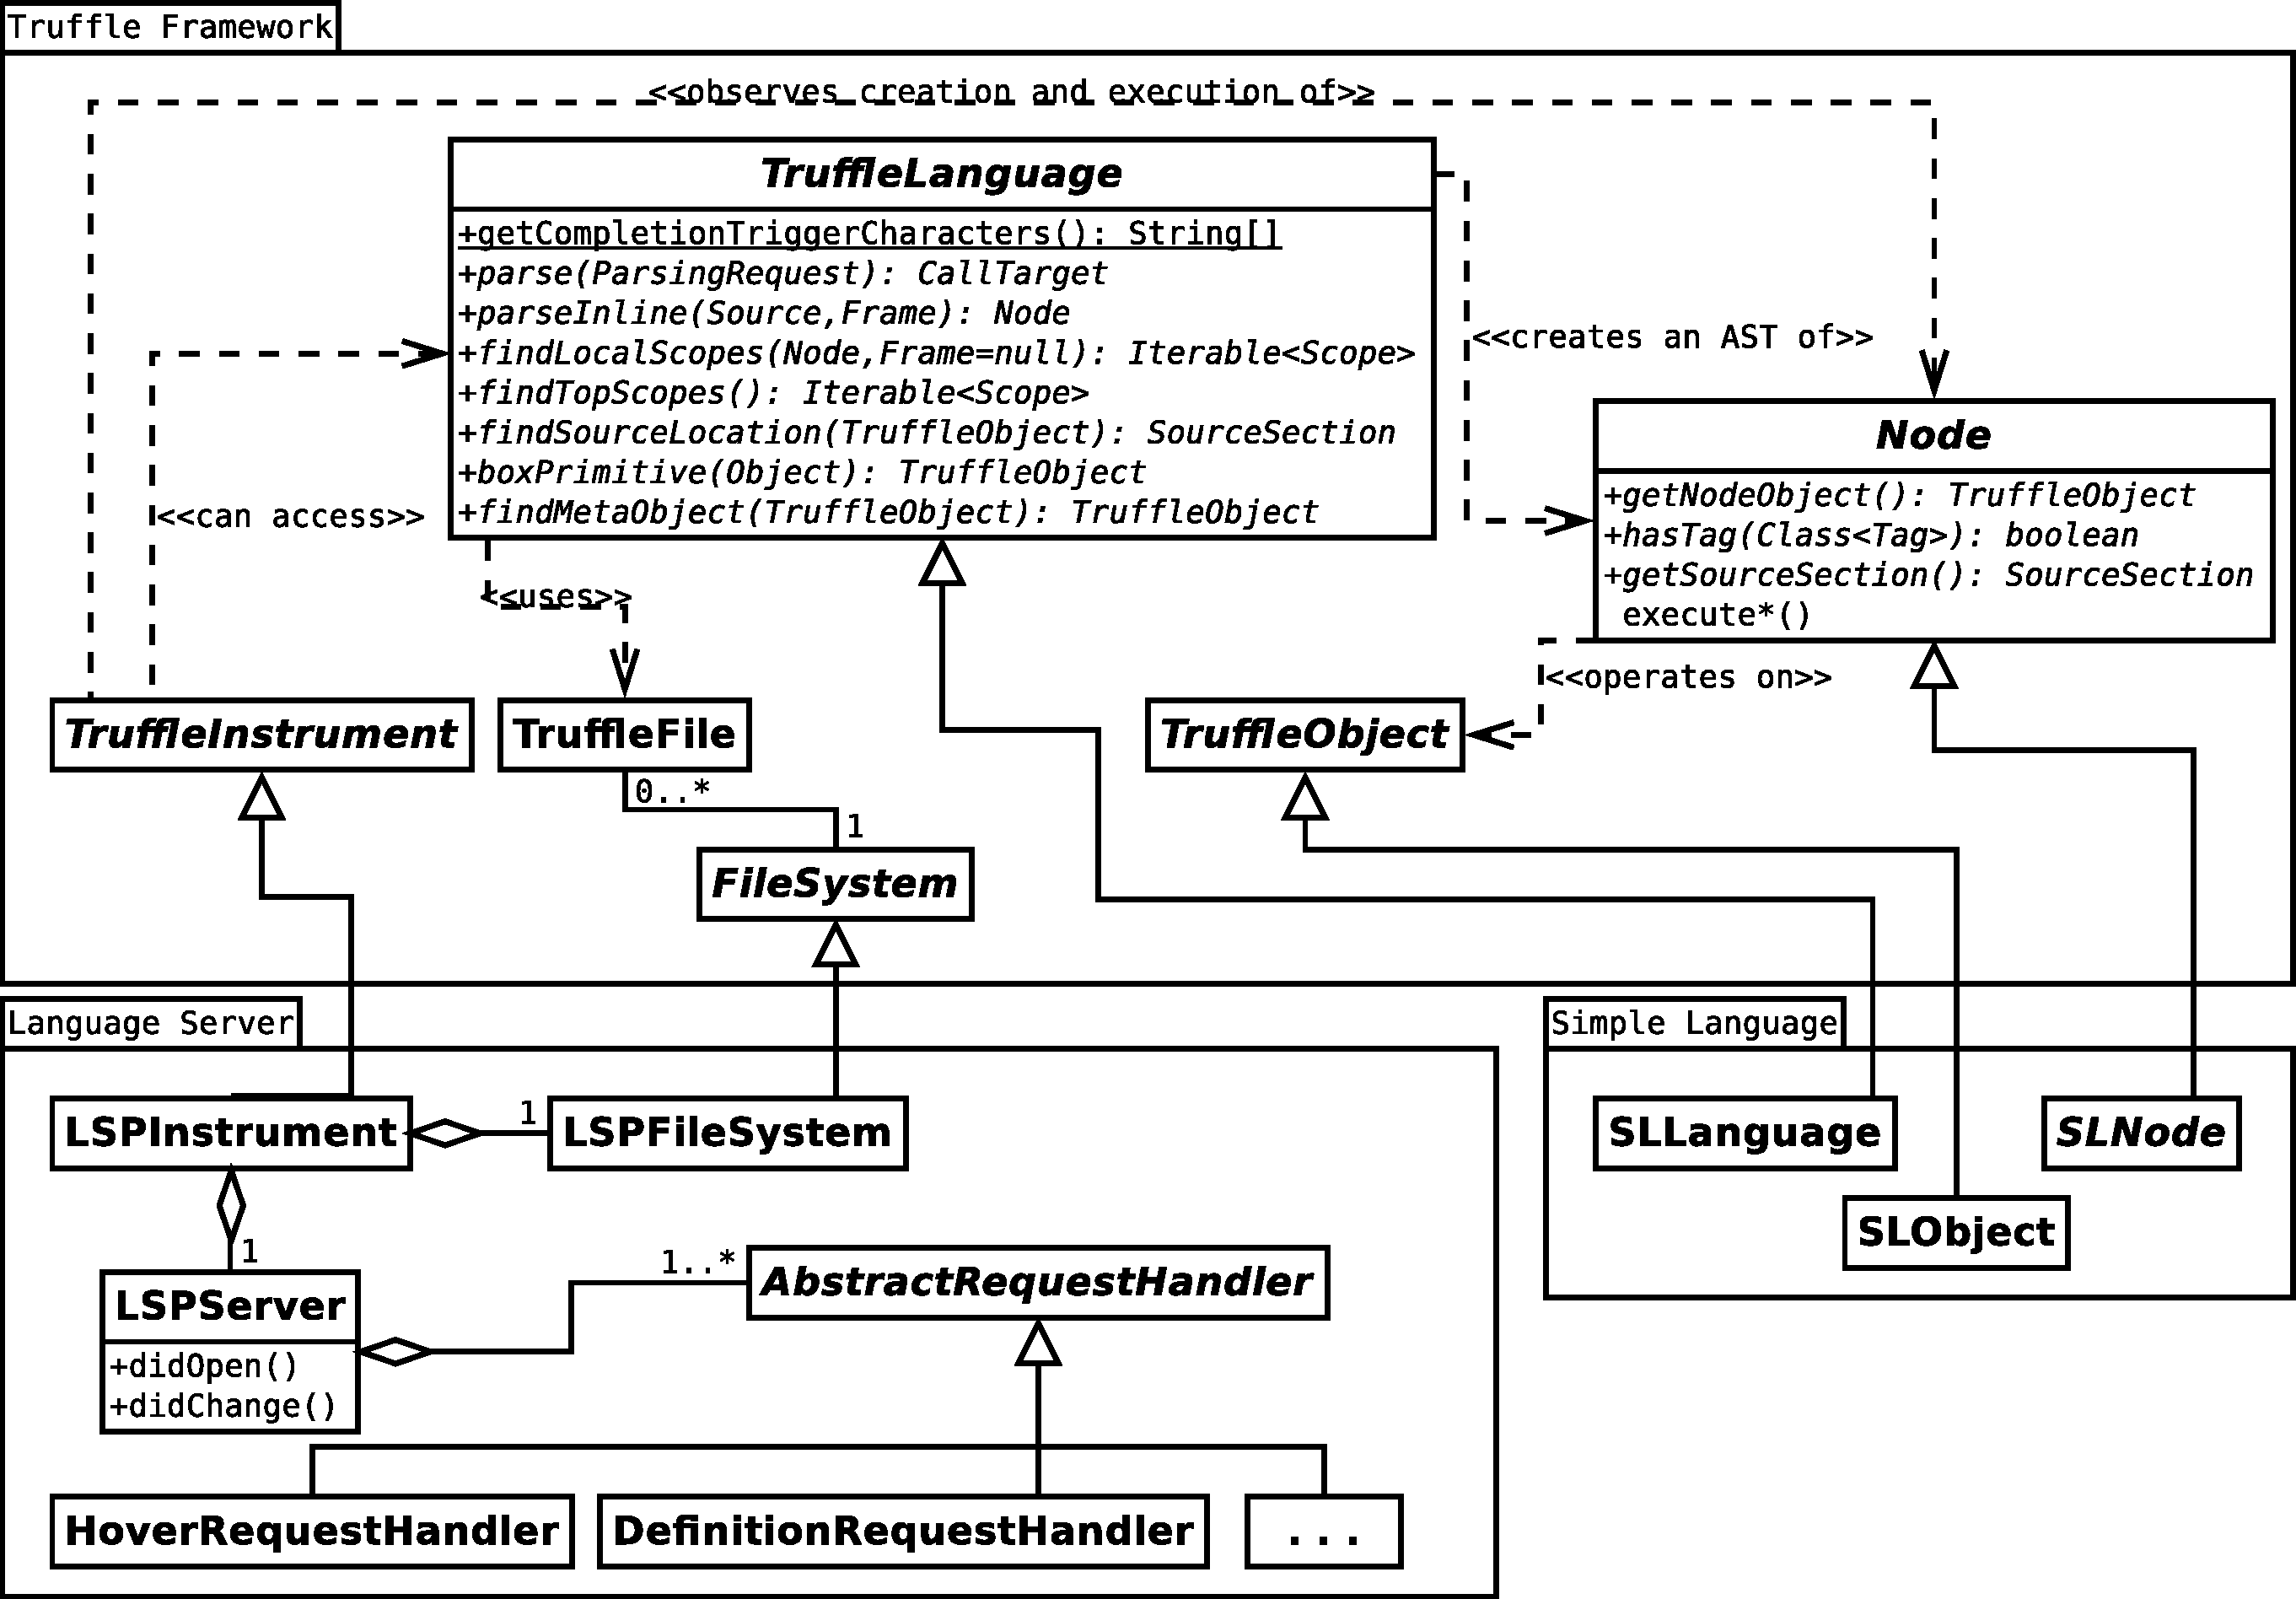
\includegraphics[width=0.6\linewidth]{diagram1}
  \caption{\DIFaddFL{Simplified Class Diagram of LSP Components, Truffle, and
    }\textsc{\DIFaddFL{SL}}}
  \label{fig:uml}
\end{figure*}
\DIFaddend 

\DIFdelbegin \paragraph{\DIFdel{Detecting an Object Property Completion}}
    %DIFAUXCMD
\addtocounter{paragraph}{-1}%DIFAUXCMD
\DIFdel{As prerequisite for
completion of properties, we need to be able to query a language implementation for its completion trigger characters. When a completion request arrives, we can then distinguish the two kinds of completion by comparing one or multiple characters directly in front of the completion request position with the trigger characters of the
current language. If there is a match, we try a property completion. To support auto-activation of code completion, the trigger characters need to be sent to the client as part of the }\emph{\DIFdel{initialize}} %DIFAUXCMD
\DIFdel{response}\DIFdelend \DIFaddbegin \DIFadd{Specific to our instrument is that it launches an HTTP server on creation. This
}\inlinecode{LSPServer} \DIFadd{handles the client's \mbox{%DIFAUXCMD
\ac{lsp} }\hspace{0pt}%DIFAUXCMD
requests. The handlers for
the various requests are where the features we describe in this section are
implemented. Whenever a file is touched, the }\inlinecode{didOpen} \DIFadd{and
}\inlinecode{didChange} \DIFadd{callback uses the languages to }\inlinecode{parse} \DIFadd{the
source. This immediately provides syntax errors and records any created \mbox{%DIFAUXCMD
\ac{ast}
}\hspace{0pt}%DIFAUXCMD
nodes. These recorded nodes are then used in subsequent requests to map from
editing locations to the \mbox{%DIFAUXCMD
\ac{ast}}\hspace{0pt}%DIFAUXCMD
, by filtering on the results of
}\inlinecode{getSourceSection}\DIFaddend .

\paragraph{\DIFdelbegin \DIFdel{Finding the Desired Node}\DIFdelend \DIFaddbegin \DIFadd{Navigational Features}\DIFaddend }
\DIFdelbegin \DIFdel{To find an \mbox{%DIFAUXCMD
\ac{ir}}\hspace{0pt}%DIFAUXCMD
-element in front of
the completion trigger character, }\DIFdelend \DIFaddbegin 

\subparagraph{\DIFadd{Symbols}} \DIFadd{The }\emph{\DIFadd{documentSymbol}} \DIFadd{and }\emph{\DIFadd{symbol}} \DIFadd{requests of
the \mbox{%DIFAUXCMD
\ac{lsp} }\hspace{0pt}%DIFAUXCMD
ask for known names and their locations on }\DIFaddend the source code\DIFdelbegin \DIFdel{needs to be parsable. We assume, that this is not always the case when a completion is triggered, because an inserted completion character might cause a syntax error. Therefore, we suggest to revert the last textual change which was sent from the client via the }\emph{\DIFdel{didChange}} %DIFAUXCMD
\DIFdel{notification and then try to
parse the reverted source code again. Translated to our Python example in }%DIFDELCMD < \autoref{lst:pythonObjectPropertyCompletion1NewApproach}%%%
\DIFdel{, the source code shown is no valid Python source code because of the last dot. Removing this dot makes the code parsable again. %DIF <  \todo{add remark: approach only possible for languages which support "expression statements"? <- how can we name that? For example in Java this would not work.}
}\DIFdelend \DIFaddbegin \DIFadd{. For
functions, this already works for all file-based Truffle languages. After
parsing, our instrument was notified of any }\emph{\DIFadd{root}} \DIFadd{node (e.g. of a
function) and can use its }\inlinecode{getSourceSection} \DIFadd{method. The language
developer has to implement this method, but this is already required for other
Truffle tools and thus did not need additional support.
}\DIFaddend 

\DIFdelbegin \DIFdel{Now, we can search for a matching \mbox{%DIFAUXCMD
\ac{ir}}\hspace{0pt}%DIFAUXCMD
-element in front of the removed completion trigger character position, by checking its lexical source section. However, there might be multiple \mbox{%DIFAUXCMD
\ac{ir}}\hspace{0pt}%DIFAUXCMD
-elements whose lexical source sections end before the removed trigger character position. Furthermore, we are only interested in an \mbox{%DIFAUXCMD
\ac{ir}}\hspace{0pt}%DIFAUXCMD
-element which represents an expression,
because we want to obtain its result. Hence, we assume again, that language implementations can expose meta-information of \mbox{%DIFAUXCMD
\ac{ir}}\hspace{0pt}%DIFAUXCMD
-elements through the framework, so that we can filter for example for expressions only}\DIFdelend \DIFaddbegin \DIFadd{We have extended the list of tags that Truffle uses to identify the purpose of
\mbox{%DIFAUXCMD
\ac{ast} }\hspace{0pt}%DIFAUXCMD
nodes with a }\emph{\DIFadd{DeclarationTag}}\DIFadd{. For \mbox{%DIFAUXCMD
\ac{sl}}\hspace{0pt}%DIFAUXCMD
, we needed to extend
the }\inlinecode{hasTag} \DIFadd{method in those nodes that introduce variables to
respond true for that tag to have them show up in the list of symbols. For
additional information, we also made use of the }\inlinecode{getNodeObject} \api
\DIFadd{provided by Truffle nodes. The convention we chose is that, if the language
developer returns an object from this method for a node tagged as a declaration,
that object can respond to the }\inlinecode{kind} \DIFadd{message with more detailed
information about the declared variable. This allows languages to communicate
statically known types if possible. For \mbox{%DIFAUXCMD
\ac{sl}}\hspace{0pt}%DIFAUXCMD
, we here return the primitive
type or }\inlinecode{object} \DIFadd{if the RHS of the assignment is a constant}\DIFaddend .

\DIFdelbegin \paragraph{\DIFdel{Obtaining the Actual Properties}}
    %DIFAUXCMD
\addtocounter{paragraph}{-1}%DIFAUXCMD
\DIFdel{To get the expression result, we need to execute the corresponding \mbox{%DIFAUXCMD
\ac{ir}}\hspace{0pt}%DIFAUXCMD
-element. In our Python example, we would evaluate an \mbox{%DIFAUXCMD
\ac{ir}}\hspace{0pt}%DIFAUXCMD
-element representing a variable read for the symbol }%DIFDELCMD < \inlinecode{natural}%%%
\DIFdel{. We can use the
already described approach for obtaining run-time information for locals, to execute the source code until the
desired \mbox{%DIFAUXCMD
\ac{ir}}\hspace{0pt}%DIFAUXCMD
-element is reached. Then, the framework needs to
provide an \mbox{%DIFAUXCMD
\ac{api}}\hspace{0pt}%DIFAUXCMD
, so that we can intercept the result of the \mbox{%DIFAUXCMD
\ac{ir}}\hspace{0pt}%DIFAUXCMD
-element execution. Having the run-time object, we need the support of the framework to query the language implementation for properties of that object, together with further meta-information of these properties, to add details, kind, and documentation for each completion item.
}\DIFdelend %DIF >  as shown for GraalPython in \autoref{fig:xp:symbolsPython}.

\DIFdelbegin \DIFdel{We suggest some optimizations to avoid executing source code for every property completion request. First of
all, we can optimize property completion for literals, if the framework supports identifying \mbox{%DIFAUXCMD
\ac{ir}}\hspace{0pt}%DIFAUXCMD
-elements as literal representations. The literal value is typically encoded in or referenced by the \mbox{%DIFAUXCMD
\ac{ir}}\hspace{0pt}%DIFAUXCMD
-element. If we can access this value}\DIFdelend %DIF >      \begin{figure}
%DIF >        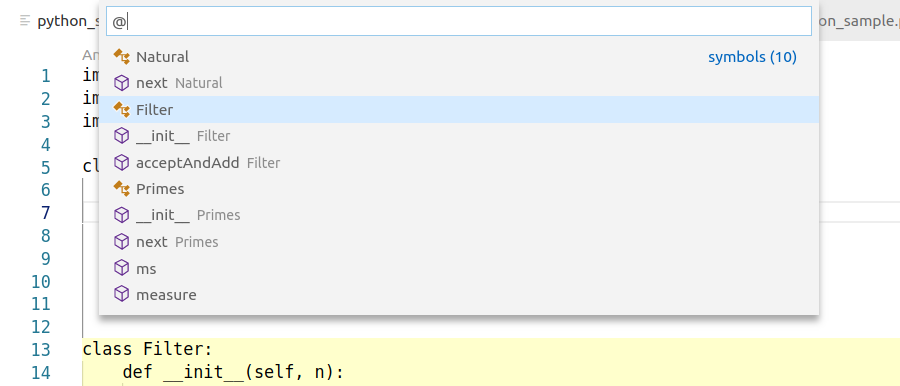
\includegraphics[width=\linewidth]{images/xp_report/symbols_Python.png}
%DIF >        \caption[Symbol overview in GraalPython]{Symbol overview over the current GraalPython document. The selected entry's source section is highlighted in the editor.}
%DIF >        \label{fig:xp:symbolsPython}
%DIF >      \end{figure}
\DIFaddbegin 

\subparagraph{\DIFadd{Go to definition}}
\DIFadd{When the user selects a function name and asks for the }\emph{\DIFadd{definition}}
\DIFadd{location, we can attempt to provide a static location or a dynamic one. In the
static case, we only need to search the \mbox{%DIFAUXCMD
\ac{ast} }\hspace{0pt}%DIFAUXCMD
for a node representing the
function call. These are already tagged in \mbox{%DIFAUXCMD
\ac{sl} }\hspace{0pt}%DIFAUXCMD
with the }\emph{\DIFadd{CallTag}} \DIFadd{to
support the Chrome debugger. From that node we match the name of the function
call to function definitions that have been parsed to show a list of
candidates. Similarly, given our newly introduced }\emph{\DIFadd{DeclarationTag}}\DIFaddend , we can
\DIFdelbegin \DIFdel{directly query for its properties}\DIFdelend \DIFaddbegin \DIFadd{also query the definition locations of variables with a certain name}\DIFaddend .

If \DIFdelbegin \DIFdel{the \mbox{%DIFAUXCMD
\ac{ir}}\hspace{0pt}%DIFAUXCMD
-element is not representing a literal, we can check as next step if there are already cached }\DIFdelend \DIFaddbegin \DIFadd{we are able to gather }\DIFaddend run-time information \DIFdelbegin \DIFdel{available. If the framework and the language implementation support in-line evaluation, we can execute the \mbox{%DIFAUXCMD
\ac{ir}}\hspace{0pt}%DIFAUXCMD
-element in the context of the cached information. }%DIFDELCMD < 

%DIFDELCMD <     %%%
\DIFdel{If there are no cached run-time information available, we need to execute unit tests or }\DIFdelend \DIFaddbegin \DIFadd{we can provide more accurate
information. To gather runtime data, we send another }\inlinecode{parse} \DIFadd{request
to the language and execute the resulting call target. This parse request either
contains some unit test or other entry point declared by the user, or just }\DIFaddend the
current source \DIFdelbegin \DIFdel{code until the \mbox{%DIFAUXCMD
\ac{ir}}\hspace{0pt}%DIFAUXCMD
-element is reached,
to get the required run-time object}\DIFdelend \DIFaddbegin \DIFadd{file as described in
}\autoref{sec:newApproachCompletionLocalsUsingRuntimeInfo}\DIFadd{. Without runtime data,
we fall back to calling }\inlinecode{findTopScopes} \DIFadd{and looking for the name
there}\DIFaddend .

\DIFdelbegin \DIFdel{If there is still no result, because the source position of the completion request might not be reachable or a timeout occurred, we can use a last fallback. We suggest to evaluate the \mbox{%DIFAUXCMD
\ac{ir}}\hspace{0pt}%DIFAUXCMD
-element in the global scope. This will at least provide a property completion for globals and context-independent expressions.
}%DIFDELCMD < 

%DIFDELCMD < %%%
\subsection[]{\DIFdel{Transferring the Approach to Other Requests}}
%DIFAUXCMD
\addtocounter{subsection}{-1}%DIFAUXCMD
%DIFDELCMD < \label{sec:appr:transferringApproachToOtherRequests}
%DIFDELCMD < %%%
\DIFdel{The approach of supporting code completion, described in the previous sections,
includes parts that can be used to support further \mbox{%DIFAUXCMD
\ac{lsp} }\hspace{0pt}%DIFAUXCMD
requests. In our
opinion, these additional requests we have chosen to highlight here are part of
the essential feature set of an \mbox{%DIFAUXCMD
\ac{de} }\hspace{0pt}%DIFAUXCMD
for dynamic languages.
%DIF <  These are:
%DIF <  \begin{description}
%DIF <  \item[documentSymbol] Request for symbols of a specific source file (function
%DIF <    names, variable names, module names, etc.)
%DIF <  \item[symbol] Like documentSymbol, but for all files in the client workspace.
%DIF <  \item[signatureHelp] Request to find signature information (e.g. parameter names
%DIF <    and details for a function) at caret position. Is triggered via registered
%DIF <    trigger characters.
%DIF <  \item[hover] Request for information at caret-hovering position.
%DIF <  \item[definition] Goto-definition request for functions, variables, etc.
%DIF <  \item[references] Request to find all references of a symbol.
%DIF <  \item[documentHighlight] Request to highlight all ranges related to a symbol
%DIF <    (e.g. variable reads and writes).
%DIF <  \item[rename] Request to rename a symbol workspace-wide.
%DIF <  \end{description}
}\DIFdelend \DIFaddbegin \DIFadd{We use the }\inlinecode{TruffleLanguage\#findSourceLocation} \api\DIFadd{, which
language developers can implement to provide the definition location of
objects where it is convenient to provide. For most languages including
\mbox{%DIFAUXCMD
\ac{sl}}\hspace{0pt}%DIFAUXCMD
, function objects are supported by this }\api \DIFadd{and we can thus
unambiguously determine the definition of a function call even when there are
multiple functions with the same name.
}\DIFaddend 

%DIF <  \autoref{tab:furtherLSPFeatures} shows the selected \ac{lsp} requests,
%DIF <  for which we will describe the approach transfer in the following. We have
%DIF <  chosen these requests, because they
\DIFaddbegin \subparagraph{\DIFadd{References}}
\DIFaddend 

\DIFdelbegin \DIFdel{In particular, we will highlight how to support }\DIFdelend \DIFaddbegin \DIFadd{For the }\DIFaddend \emph{\DIFdelbegin \DIFdel{hover}\DIFdelend \DIFaddbegin \DIFadd{documentHighlight}\DIFaddend } \DIFdelbegin \DIFdel{, }\emph{\DIFdel{definition}}%DIFAUXCMD
\DIFdel{,
}\DIFdelend and \emph{references} \DIFdelbegin \DIFdel{requests for callables and local variables, the
}\emph{\DIFdel{signatureHelp}} %DIFAUXCMD
\DIFdel{request for callables, and the }\emph{\DIFdel{documentHighlight}} %DIFAUXCMD
\DIFdel{and
}\emph{\DIFdel{rename}} %DIFAUXCMD
\DIFdel{requests for local variables only}\DIFdelend \DIFaddbegin \DIFadd{\mbox{%DIFAUXCMD
\ac{lsp} }\hspace{0pt}%DIFAUXCMD
messages, we
re-use the CallTag and DeclarationTag annotations to find nodes with the names
we are interested in}\DIFaddend . Furthermore, we \DIFdelbegin \DIFdel{will highlight,
how to support the }\DIFdelend \DIFaddbegin \DIFadd{have added two more tags,
}\DIFaddend \emph{\DIFdelbegin \DIFdel{symbol}\DIFdelend \DIFaddbegin \DIFadd{ReadVariableTag}\DIFaddend } and \emph{\DIFdelbegin \DIFdel{documentSymbol}%DIFDELCMD < \MBLOCKRIGHTBRACE %%%
\DIFdel{requests for any kind
of symbol declaration. As already described for code completion, we rely on
meta-information exposed by the language implementation framework. This
information allows us to search for certain kinds of \mbox{%DIFAUXCMD
\ac{ir}}\hspace{0pt}%DIFAUXCMD
-elements
representing a call to a callable or an access to a variable at the requested
position, or to retrieve all kind of symbol declarations in a source code file. }\DIFdelend \DIFaddbegin \DIFadd{WriteVariableTag}}\DIFadd{, which we have added to nodes
representing local variable accesses in \mbox{%DIFAUXCMD
\ac{sl}}\hspace{0pt}%DIFAUXCMD
. Together, these allow us to
return references for variables and functions.
}

\DIFadd{To take scopes into account, we make use of another Truffle }\api \DIFadd{that is already
implemented in \mbox{%DIFAUXCMD
\ac{sl}}\hspace{0pt}%DIFAUXCMD
, }\inlinecode{findLocalScopes}\DIFadd{, which enumerates scopes
from the inside out. If, for example, the client asks to highlight all
references to a variable in a closure, the local scope }\api \DIFadd{will enumerate
surrounding scopes up to the top scope. Our server can then search for the same
names in those scopes and find the correspondingly tagged notes. This }\api \DIFadd{can
be used statically or with a run-time }\inlinecode{Frame} \DIFadd{object, and returns
lexical scope or dynamic scope nesting, respectively.
}\DIFaddend 

%DIF <  \begin{table*}
    %DIF <      \centering
    %DIF <      % \tableinsidecommand
    %DIF <      \begin{threeparttable}
    %DIF <        \caption[Selected \acs{lsp} features and their descriptions]{Selected \acs{lsp} features and their descriptions.}
    %DIF <        \label{tab:furtherLSPFeatures}
    %DIF <        \begin{tabular}{ l p{0.5\linewidth} }
    %DIF <          \toprule
    %DIF <          Request/Notification    & Description\\
    %DIF <          \midrule
    %DIF <          documentSymbol          & Request for symbols of a specific source file (function names, variable names, module names, etc.).  \\
    %DIF <          symbol                  & Like documentSymbol, but for all files in the client workspace. \\
    %DIF <          signatureHelp           & Request to find signature information (e.g. parameter names and details for a function) at caret position. Is triggered via registered trigger characters.     \\
    %DIF <          hover                   & Request for information at caret-hovering position.\\
    %DIF <          definition              & Goto-definition request for functions, variables, etc. \\
    %DIF <          references              & Request to find all references of a symbol. \\
    %DIF <          documentHighlight       & Request to highlight all ranges related to a symbol (e.g. variable reads and writes).     \\
    %DIF <          rename                  & Request to rename a symbol workspace-wide.     \\
    %DIF <          \bottomrule
    %DIF <        \end{tabular}
    %DIF <      \end{threeparttable}
    %DIF <  \end{table*}
%DIF >  \paragraph{Renaming}
%DIF >  \subparagraph{} Renaming of a function, for example, requires us to determine
%DIF >  its definition as well as all references to that function. While our approach to
%DIF >  finding these fall back to potentially ambiguous static searches as explained
%DIF >  above, for renaming we only answer the request of the client if we have run-time
%DIF >  information available for all locations that we find statically to reference the
%DIF >  same name. We do this to avoid potentially incorrect or incomplete modifications
%DIF >  to the source code. As such, renaming support is currently limited to sources
%DIF >  that have good coverage from dynamic code execution.

%DIF < \todo{Zusammenfassung, was wiederverwendet werden kann: run-to-section + static search for tagged \ac{ir}-elements + \ac{ir}-element lexical source section}
\DIFaddbegin \paragraph{\DIFadd{Informational Features}}
\DIFaddend 

\DIFdelbegin \paragraph{\DIFdel{Document and Workspace Symbols}}
    %DIFAUXCMD
\addtocounter{paragraph}{-1}%DIFAUXCMD
%DIF <  \begin{itemize}
    %DIF <      \item response: range + kind + container
    %DIF <      \item scan all \ac{ir}-elements for those representing a symbol definition, e.g. via tagging
    %DIF <      \item use lexical source section of \ac{ir}-element
    %DIF <  \end{itemize}
    \DIFdel{The }\emph{\DIFdel{documentSymbol}} %DIFAUXCMD
\DIFdel{and }\emph{\DIFdel{symbol}} %DIFAUXCMD
\DIFdel{response items consist of a label, range, symbol kind, and container name.
To provide this information, we assume that the language implementations can expose this information through the framework. }\DIFdelend \DIFaddbegin \subparagraph{\DIFadd{Detecting syntax errors}}
\DIFaddend 

\DIFdelbegin \DIFdel{First of all, we need to collect all
\mbox{%DIFAUXCMD
\ac{ir}}\hspace{0pt}%DIFAUXCMD
-elements for a source code file, which define a symbol. Having them, label, range and symbol kind could be derived from the \mbox{%DIFAUXCMD
\ac{ir}}\hspace{0pt}%DIFAUXCMD
-element and its lexical source section. The container name could be derived from the names of the surrounding lexical scopes.
To support the workspace-wide }\emph{\DIFdel{symbol}} %DIFAUXCMD
\DIFdel{request, we can build the union of }\emph{\DIFdel{documentSymbol}} %DIFAUXCMD
\DIFdel{requests for all files in the
workspace}\DIFdelend \DIFaddbegin \DIFadd{Language runtime parsers are not usually built to support incremental parsing or
detection of more than one syntax error. \mbox{%DIFAUXCMD
\ac{sl}}\hspace{0pt}%DIFAUXCMD
, like other Truffle languages,
fails parsing at the first syntax error, so that only one error per file can be
sent to the client. By convention, a language syntax error is supposed to
implement the }\inlinecode{TruffleException} \DIFadd{interface (not shown in the
diagram), which provides a }\inlinecode{getSourceLocation}
\DIFadd{method. }\autoref{fig:xp:diagnosticsSL} \DIFadd{displays how such a diagnostics
notification is visualized in \mbox{%DIFAUXCMD
\ac{sl}}\hspace{0pt}%DIFAUXCMD
}\DIFaddend .

\DIFdelbegin \paragraph{\DIFdel{Signature Help and Goto-definition for Callables}}
    %DIFAUXCMD
\addtocounter{paragraph}{-1}%DIFAUXCMD
\DIFdelend \DIFaddbegin \begin{figure}
  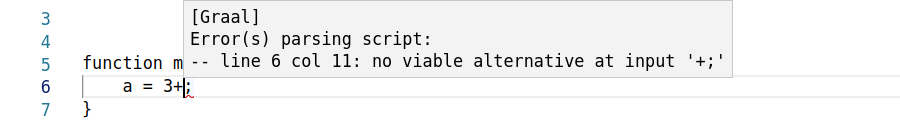
\includegraphics[width=\linewidth]{images/xp_report/diagnostics_sl.png}
  \caption[Diagnostics used to display a syntax error in \acs{sl}]{\DIFaddFL{Diagnostics used to display a syntax error in \acs{sl}.}}
  \label{fig:xp:diagnosticsSL}
\end{figure}

\subparagraph{\DIFadd{Documentation and signature help}}

\DIFaddend The \emph{signatureHelp} request is auto-activated at client-side, like code
completion, if the server includes trigger characters for signature help in the
\emph{initialize} response. A \emph{signatureHelp} response consists of a list
of signatures, because there might be different variants, if the language
implementation supports function overloading.
\DIFdelbegin \DIFdel{Furthermore, the response includes two indices, telling which signature and
which parameter should be shown in detail in the UI.
Every signature in the list consists of a label, a list of parameters, and an optional documentation. A parameter also consists of label and documentation}\DIFdelend \DIFaddbegin 

\DIFadd{If we can gather run-time information to access the object representing the
function on the Truffle level, we have added two }\api \DIFadd{messages that the language
developer needs to implement: }\inlinecode{GetDocumentation} \DIFadd{and
}\inlinecode{GetSignature}\DIFadd{. These should return a documentation string or all
parameter names and their documentation, respectively. The formatting of these
is language specific and left to the language developer.
}

\DIFadd{If we either cannot gather run-time information or the additional }\api \DIFadd{is not
implemented by the language, we fall back to trying to find the definition of
the function (as described above) and show the surrounding source code as a hint
to the developer.
}

\DIFadd{\mbox{%DIFAUXCMD
\ac{sl} }\hspace{0pt}%DIFAUXCMD
does not keep track of documentation strings in its parser, and neither
does the parser keep parameter names separate from local variables. Implementing
these two messages will require more work in the parser of \mbox{%DIFAUXCMD
\ac{sl}}\hspace{0pt}%DIFAUXCMD
}\DIFaddend .

\DIFdelbegin \DIFdel{To collect all the needed information, we suggest the following steps. }\DIFdelend \DIFaddbegin \subparagraph{\DIFadd{Hover information}}
\DIFaddend 

\DIFdelbegin %DIFDELCMD < \begin{enumerate}
%DIFDELCMD <         \item %%%
\DIFdel{Find an \mbox{%DIFAUXCMD
\ac{ir}}\hspace{0pt}%DIFAUXCMD
-element representing a call to a }\DIFdelend \DIFaddbegin \DIFadd{We can support the }\emph{\DIFadd{hover}} \DIFadd{request to show information for variables and
callables with type information, provided there is run-time information
available. If we have found an \mbox{%DIFAUXCMD
\ac{ast} }\hspace{0pt}%DIFAUXCMD
node representing a variable or }\DIFaddend callable
at the requested position\DIFdelbegin %DIFDELCMD < \item %%%
\DIFdel{Execute the
source code until the \mbox{%DIFAUXCMD
\ac{ir}}\hspace{0pt}%DIFAUXCMD
-element is reached
        }%DIFDELCMD < \item %%%
\DIFdel{Intercept the callable run-time object represented by the \mbox{%DIFAUXCMD
\ac{ir}}\hspace{0pt}%DIFAUXCMD
-element
        }%DIFDELCMD < \item %%%
\DIFdel{Query the callable for label, parameters and
documentation
    }%DIFDELCMD < \end{enumerate}
%DIFDELCMD < %%%
\DIFdelend \DIFaddbegin \DIFadd{, we use }\inlinecode{parseInline} \DIFadd{and evaluate the
resulting node. With the result, we build the hover response. Most Truffle
languages including \mbox{%DIFAUXCMD
\ac{sl} }\hspace{0pt}%DIFAUXCMD
already implement the }\inlinecode{findMetaObject}
\api\DIFadd{. We use it on the result to show the type here in addition to the concrete
value.
}\DIFaddend 

\DIFdelbegin \DIFdel{The first to third steps equal those for }\DIFdelend %DIF >  \begin{figure}
%DIF >      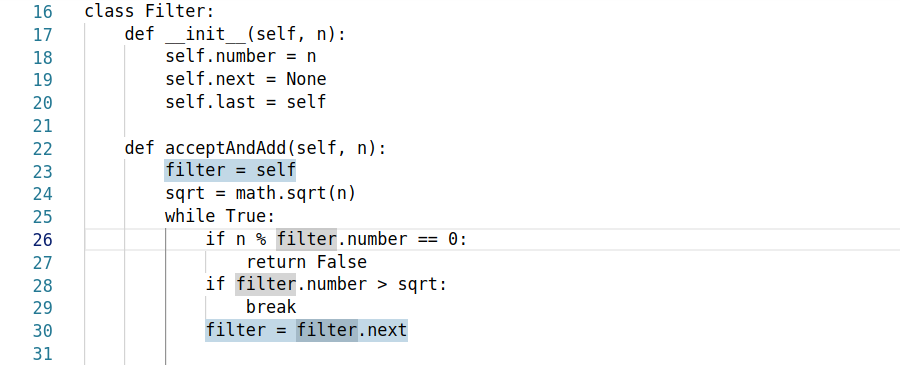
\includegraphics[width=\linewidth]{images/xp_report/highlighting_Python.png}
%DIF >      \caption[Highlighting of variable accesses in GraalPython]{Highlighting of variable accesses in GraalPython. The source sections of write accesses cover the whole assignment and are highlighted in a blueish shade.}
%DIF >      \label{fig:xp:highlightingPython}
%DIF >  \end{figure}
\DIFaddbegin 

\paragraph{\DIFadd{Completion}}
\label{sec:newApproach:completionOfGlobals}

\subparagraph{}
\DIFadd{We distinguish two kinds of code completions which need
different levels of support by the language: completion of globals or locals and
completion of properties.
}

\subparagraph{\DIFadd{Globals and locals}} \DIFadd{We use the code snippet in
}\autoref{lst:pythonNearCaretExample1NewApproach} \DIFadd{to illustrate how to support
}\DIFaddend code completion of \DIFdelbegin \DIFdel{properties. A challenge is, that the signature help should be displayed from the time, the trigger character is inserted, until
the user has completed the signature. During that process, the source code might contain syntax errors, so that we have no \mbox{%DIFAUXCMD
\ac{ir}}\hspace{0pt}%DIFAUXCMD
-elements. Returning an empty response will end the displayed signature help. Therefore, this request might be supported only partial, depending on the particular language syntax. }%DIFDELCMD < 

%DIFDELCMD <     %%%
\DIFdel{Having obtained a callable object, the last step implies, that we can query the framework for information about that callable. Among all parameter names and their documentation, we need a formatted, language-specific representation of signature to create the label. If this is not supported by the framework, but we can get at least access to }\DIFdelend \DIFaddbegin \DIFadd{globals and locals. With the caret on line 3, }\DIFaddend a
\DIFdelbegin \DIFdel{list of parameter names, we suggest to use a Python-like syntax }%DIFDELCMD < \inlinecode{callableName(param1, param2, paramN)} %%%
\DIFdel{as signature label. }%DIFDELCMD < 

%DIFDELCMD <     %%%
\DIFdel{The approach to
support the }\emph{\DIFdel{definition}} %DIFAUXCMD
\DIFdel{request for callables is
quite similar. Only in the last step, we do not have to query the framework for signature information, but for the callable's definition location in the source code.
Furthermore, we can apply a static search as fallback, if the dynamic approach does not yield a result. We can use the
same approach as for the }\emph{\DIFdel{symbol}} %DIFAUXCMD
\DIFdel{request }\DIFdelend \DIFaddbegin \emph{\DIFadd{completion}} \DIFadd{request is sent to the server for line 3 at character offset
4. The server searches the parsed nodes for the one with the nearest
}\inlinecode{SourceSection} \DIFadd{and uses it to call }\inlinecode{findTopScopes} \DIFadd{and
}\inlinecode{findLocalScopes}\DIFadd{. We would expect a completion result to include
items for all \mbox{%DIFAUXCMD
\ac{sl} }\hspace{0pt}%DIFAUXCMD
globals (e.g. built-in functions) and the locals
}\inlinecode{param1}\DIFaddend , \DIFdelbegin \DIFdel{to find all definitions of callables in the
workspace and filter those matching the identifier of the callable at the requested position. For non-unique identifiers, this might yield many results, which are not related to the desired definition location. But in our opinion, it is better to provide the users a list of potential matches instead of providing nothing. }\DIFdelend \DIFaddbegin \inlinecode{param2}\DIFadd{, and }\inlinecode{x}\DIFadd{. The variable
}\inlinecode{y} \DIFadd{should not be included, because no value is assigned to it until
line 4. %DIF >  Besides a display name, a \ac{lsp} completion item can optionally
%DIF >  contain a completion kind (e.g. variable, function, or class), a detail text for
%DIF >  signature or type information, and a documentation.
}\DIFaddend 

\DIFdelbegin \paragraph{\DIFdel{Document Highlight, Rename and Find All References}}
    %DIFAUXCMD
\addtocounter{paragraph}{-1}%DIFAUXCMD
\DIFdel{The }\emph{\DIFdel{documentHighlight}}%DIFAUXCMD
\DIFdel{, }\emph{\DIFdel{rename}} %DIFAUXCMD
\DIFdel{and the }\emph{\DIFdel{references}}
    %DIFAUXCMD
\DIFdel{responses consist of a list of ranges in the source code. For the
    }\emph{\DIFdel{documentHighlight}} %DIFAUXCMD
\DIFdel{response, each range can additionally have an
    associated kind (}%DIFDELCMD < \inlinecode{Text}%%%
\DIFdelend \DIFaddbegin \DIFadd{Statically, we get the names and values of \mbox{%DIFAUXCMD
\ac{sl} }\hspace{0pt}%DIFAUXCMD
built-ins in the top
scopes. The values are }\inlinecode{SLObject}\DIFadd{s, so we can use the normal
}\inlinecode{TruffleObject} \DIFadd{messages to query if they are }\emph{\DIFadd{callable}}\DIFaddend ,
\DIFdelbegin %DIFDELCMD < \inlinecode{Read}%%%
\DIFdel{, or
    }%DIFDELCMD < \inlinecode{Write}%%%
\DIFdel{), and for the }\emph{\DIFdel{rename}} %DIFAUXCMD
\DIFdel{response, each range needs an
    associated file \mbox{%DIFAUXCMD
\ac{uri} }\hspace{0pt}%DIFAUXCMD
and the new text.}%DIFDELCMD < 

%DIFDELCMD <     %%%
\DIFdel{To support these requests for local variables, first of all a
    \mbox{%DIFAUXCMD
\ac{ir}}\hspace{0pt}%DIFAUXCMD
-element representing a read- or write-access of a variable at the requested positionneeds to be found. Having one, we suggest to search in the surrounding lexical scopes for all other \mbox{%DIFAUXCMD
\ac{ir}}\hspace{0pt}%DIFAUXCMD
-elements representing
    an access to
variables with the same identifier. The required range can be
    obtained from the lexical source section of the \mbox{%DIFAUXCMD
\ac{ir}}\hspace{0pt}%DIFAUXCMD
-element.
}\DIFdelend \DIFaddbegin \emph{\DIFadd{instantiable}}\DIFadd{, and so on and return appropriate flags to the client. In
languages that respond to documentation and signature messages for their
objects, we show that here as well, but there is no such support for
\mbox{%DIFAUXCMD
\ac{sl}}\hspace{0pt}%DIFAUXCMD
. }\DIFaddend For \DIFdelbegin \DIFdel{the
    }\emph{\DIFdel{documentHighlight}} %DIFAUXCMD
\DIFdel{response, the kind can be determined from the access kind of the variable. For the }\emph{\DIFdel{rename}} %DIFAUXCMD
\DIFdel{response, the \mbox{%DIFAUXCMD
\ac{uri} }\hspace{0pt}%DIFAUXCMD
is the one of the current file and the new text is
already provided in the request.
}%DIFDELCMD < 

%DIFDELCMD <     %%%
\DIFdel{Supporting }\emph{\DIFdel{references}} %DIFAUXCMD
\DIFdel{also for callables workspace-wide, we could use the same static fallback approach as described for the }\emph{\DIFdel{definition}} %DIFAUXCMD
\DIFdel{request. Due to potentially found false-positives, we do not suggest to also apply this static approach to the code-modifying }\emph{\DIFdel{rename}} %DIFAUXCMD
\DIFdel{request. }\DIFdelend \DIFaddbegin \inlinecode{findLocalScopes}\DIFadd{, \mbox{%DIFAUXCMD
\ac{sl} }\hspace{0pt}%DIFAUXCMD
statically returns the names
of }\emph{\DIFadd{all}} \DIFadd{variables defined. %DIF >  As for highlighting
%DIF >  references, we re-use the existing Truffle \api for scope enumeration here, and
%DIF >  nothing new had to be implemented.
}\DIFaddend 

\DIFdelbegin \paragraph{\DIFdel{Hover Information}}
    %DIFAUXCMD
\addtocounter{paragraph}{-1}%DIFAUXCMD
\DIFdel{We can support the }\emph{\DIFdel{hover}} %DIFAUXCMD
\DIFdel{request for variables and callables, if there are cached run-time information available. If we have found an \mbox{%DIFAUXCMD
\ac{ir}}\hspace{0pt}%DIFAUXCMD
-element representing a variable or callable at the
requested position, we can perform an in-line evaluation as described for code completion.
Using the evaluation result, we can build the hover response, by querying the framework for information about }\DIFdelend \DIFaddbegin \DIFadd{In this case example we can just execute the entire file to gather }\DIFaddend run-time
\DIFdelbegin \DIFdel{objects as described for code completion. The hover response consists of plaintext or markup content, so that we can put it together depending on the available information.
}%DIFDELCMD < 

%DIFDELCMD < %%%
%DIF < %%%%%%%%%%%%%%%%%%%%%%%%%%%%%%%%%%%%%%%%%%%%%%%%%%%%%
%DIF <  IMPLEMENTATION
%DIF < %%%%%%%%%%%%%%%%%%%%%%%%%%%%%%%%%%%%%%%%%%%%%%%%%%%%%
%DIFDELCMD < 

%DIFDELCMD < %%%
%DIF <  \section{Implementation}
%DIF <  \label{cha:implementation}
%DIFDELCMD < 

%DIFDELCMD < %%%
%DIF <      % In this chapter, we describe how we have implemented our prototype \graallsp, based on the approach described in \autoref{cha:solution}. \graallsp~uses Truffle as underlying language implementation framework and exploits Truffle's instrumentation environment to access the required information in a language-agnostic way. We also implemented a Truffle \ac{api} extension to support more \ac{lsp} features. As \ac{lsp} Java wrapper we used LSP4J. Transportation for \acs{json}-\acs{rpc} is implemented using Java's \acs{tcp} sockets. In the following sections, we start by describing how we have implemented common features required for most \ac{lsp} requests and then explain in detail the implementation of selected \ac{lsp} requests in \graallsp.
%DIFDELCMD < 

%DIFDELCMD < %%%
%DIF <      % \subsection{Prerequisites to Answer \acs{lsp} Requests with Truffle}
%DIF <          % \begin{itemize}
%DIF <          %     \item our approach has some requirements on the language impl framework
%DIF <          %     \item influences project structure and dependencies
%DIF <          %     \item server init
%DIF <          %     \item things common for most requests:
%DIF <          %     \begin{itemize}
%DIF <          %         \item parsing + diagnostics
%DIF <          %         \item mapping caret to IR
%DIF <          %         \item obtaining run-time information
%DIF <          %     \end{itemize}
%DIF <          % \end{itemize}
%DIF <      Implementing a language server on top of the Truffle framework with the requirements described in our approach, especially the sandboxing, has implications on our project structure, dependencies, and the bootstrapping process. Furthermore, there are common prerequisites to answer most \ac{lsp} requests. These are parsing source code, mapping the requested position to source sections of \ac{ast} nodes, and collecting and utilizing run-time information.
%DIFDELCMD < 

%DIFDELCMD < %%%
%DIF <      % \subsubsection{Project Structure and Dependencies}
%DIF <      % \label{sec:impl:projectStructure}
%DIF <      %     % \begin{itemize}
%DIF <      %     %     \item Building tool for Truffle = using instrumentation API
%DIF <      %     %     \item LSPInstrument loaded dynamically via class path
%DIF <      %     %     \item onCreate() we get an Env -> our entry point to parse code, find scopes etc.
%DIF <      %     %     \item For getting run-time infos we execute code -> sandboxing needed -> via creation of Truffle Context
%DIF <      %     %     \item Truffle instrument cannot create new Contexts
%DIF <      %     %     \item Need to use embedder-API -> write own launcher, create engine ourselves
%DIF <      %     %     \item set read-only file-system on context builder
%DIF <      %     %     \item Provide a callback to our instrument to create new sandboxed Contexts
%DIF <      %     %     \item lsp4j -> own threads to handle requests
%DIF <      %     %     \item Threads need to be activated for Contexts - multi-threading is not always supported
%DIF <      %     %     \item Our decision -> we have only one worker thread which enters a Context once
%DIF <      %     %     \item lsp4j thread puts work in a queue which is polled by the context aware worker thread
%DIF <      %     %     \item lsp4j threads await result via Futures
%DIF <      %     % \end{itemize}
%DIF <      %     To use Truffle's instrumentation capabilities, we have to implement the interface \inlinecode{TruffleInstrument}, which is part of the Truffle \ac{api}. Instruments are loaded via Java's \ac{spi} and the framework calls their implemented \inlinecode{onCreate(Env)} method during initialization, to pass an instance of a Truffle instrumentation environment. This environment has a language-agnostic \ac{api} to parse source code, interact with loaded languages, and observe and inject behavior into the \ac{ast} interpreters. Most \ac{lsp} features can be mapped to that \ac{api}.
        %DIFDELCMD < 

%DIFDELCMD < %%%
%DIF <          % As described in \autoref{sec:newApproachCompletionProperties}, our approach requires to sandbox the execution of guest languages and redirect file accesses. Unfortunately, the Truffle instrumentation environment provides no \ac{api} to support that requirement. However, there is a separate Graal \ac{sdk} to embed and run code from guest languages in JVM-based host applications. It allows to create and configure Polyglot \inlinecode{Engine} and Polyglot \inlinecode{Context} instances. An \inlinecode{Engine} provides access to the installed languages and instruments. A \inlinecode{Context} instance allows to evaluate code of its associated languages and represents the global run-time state. Furthermore, it supports to set a custom file system. Multiple \inlinecode{Context} instances can share the same \inlinecode{Engine} instance and thereby all its registered instruments.
        %DIFDELCMD < 

%DIFDELCMD < %%%
%DIF <      %     Therefore, we decided to create three Java projects. \autoref{fig:graalLspPackageStructure} visualizes the resulting project structure and dependencies. The first project contains a separate launcher which handles the whole bootstrapping and enables the creation of sandboxed \inlinecode{Context} instances using the Graal \ac{sdk}. The actual language server is implemented as Truffle instrument in a second project. The implementation of this instrument is shown in \autoref{lst:impl:javaLSPINstrument}. During bootstrapping, the instrument will register some services (lines 21-22) which enable the launcher for example to explicitly start the language server later. These service interfaces are part of a third project on which the others depend. 
%DIFDELCMD < 

%DIFDELCMD < %%%
%DIF <  %         \begin{code}[lst:impl:javaLSPINstrument]{[The Java class LSPInstrument]Our implementation of a \inlinecode{TruffleInstrument} used to initialize and start the language server.}{float,numbers=left,language=Java}
%DIF <  % @Registration(id = LSPInstrument.ID, name = "Language Server", version = "0.1",
%DIF <  %               services = {
%DIF <  %                 VirtualLanguageServerFileProvider.class,
%DIF <  %                 ContextAwareExecutorRegistry.class,
%DIF <  %                 LanguageServerBootstrapper.class})
%DIF <  % public class LSPInstrument extends TruffleInstrument
%DIF <  %                            implements LanguageServerBootstrapper {
%DIF <  %   public static final String ID = "lsp";
%DIFDELCMD < 

%DIFDELCMD < %%%
%DIF <  %   private OptionValues options;
%DIF <  %   private LanguageServerImpl languageServer;
%DIFDELCMD < 

%DIFDELCMD < %%%
%DIF <  %   @Override
%DIF <  %   protected void onCreate(Env env) {
%DIF <  %     options = env.getOptions();
%DIF <  %     TruffleAdapter truffleAdapter = new TruffleAdapter(env);
%DIF <  %     PrintWriter info = new PrintWriter(env.out(), true);
%DIF <  %     PrintWriter err = new PrintWriter(env.err(), true);
%DIF <  %     languageServer = LanguageServerImpl.create(truffleAdapter, info, err);
%DIFDELCMD < 

%DIFDELCMD < %%%
%DIF <  %     env.registerService(truffleAdapter);
%DIF <  %     env.registerService(this);
%DIF <  %   }
%DIFDELCMD < 

%DIFDELCMD < %%%
%DIF <  %   @Override
%DIF <  %   protected OptionDescriptors getOptionDescriptors() {
%DIF <  %     return new LSOptionsOptionDescriptors();
%DIF <  %   }
%DIFDELCMD < 

%DIFDELCMD < %%%
%DIF <  %   public Future<?> startServer() {            
%DIF <  %     HostAndPort hostAndPort = options.get(LSOptions.Lsp);
%DIF <  %     try {
%DIF <  %       InetSocketAddress socketAddress = hostAndPort.createSocket();
%DIF <  %       int port = socketAddress.getPort();
%DIF <  %       Integer backlog = options.get(LSOptions.SocketBacklogSize);
%DIF <  %       InetAddress address = socketAddress.getAddress();
%DIF <  %       ServerSocket serverSocket = new ServerSocket(port, backlog, address);
%DIF <  %       return languageServer.start(serverSocket);
%DIF <  %     } catch (IOException e) {
%DIF <  %       String message = String.format("[Graal LSP] Starting server on %s failed: %s",
%DIF <  %           hostAndPort.getHostPort(),
%DIF <  %           e.getLocalizedMessage());
%DIF <  %       throw new LSPIOException(message, e);
%DIF <  %     }
%DIF <  %   }
%DIF <  % }
%DIF <  %             \end{code}
%DIFDELCMD < 

%DIFDELCMD < %%%
%DIF <          % \begin{figure}
%DIF <          %     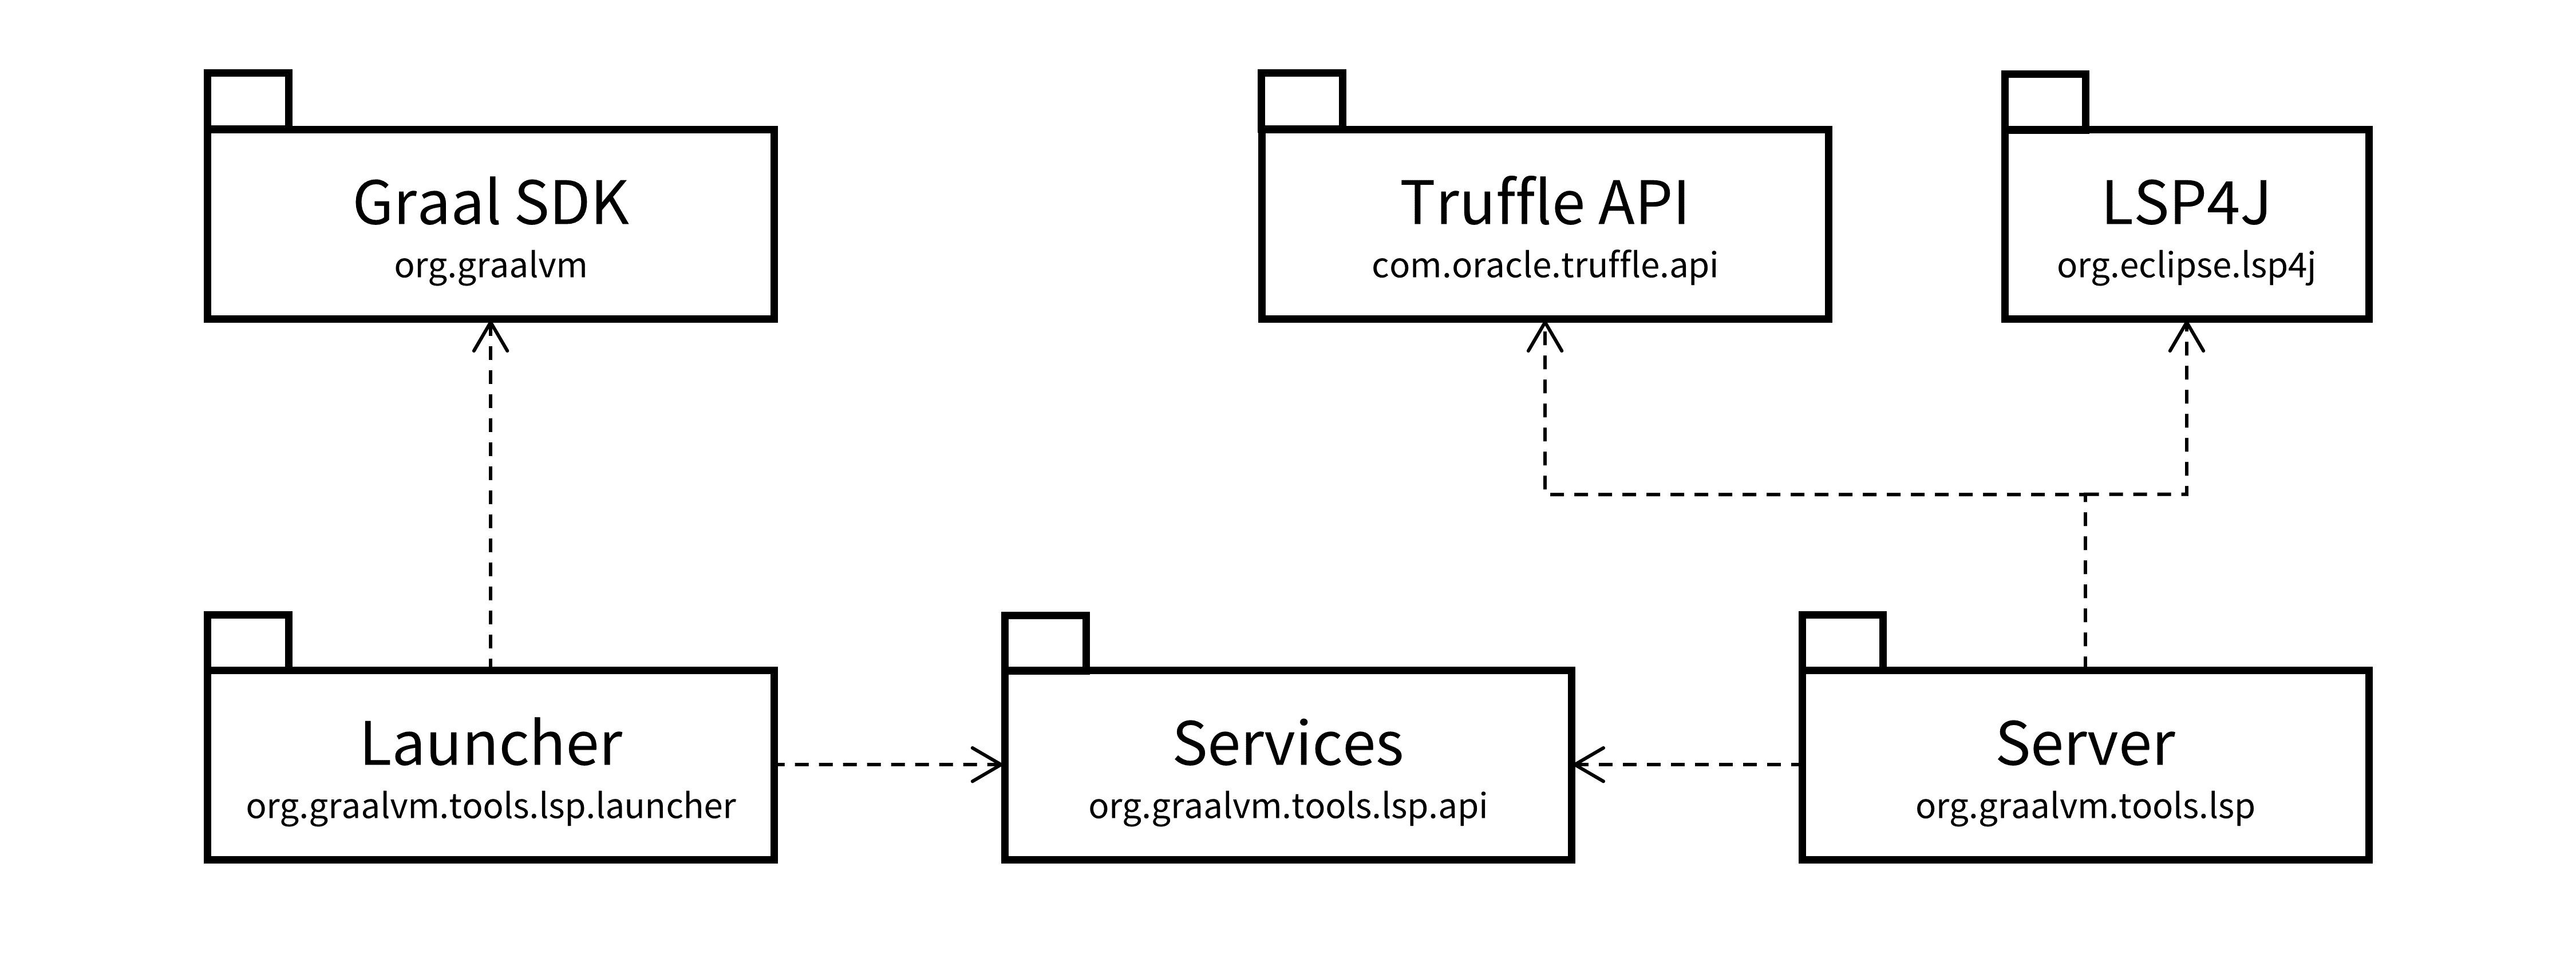
\includegraphics[width=\linewidth]{images/GraalLSP-package-structure.png}
%DIF <          %     \caption[Project structure and dependencies of \graallsp]{Project structure and dependencies of \graallsp.}
%DIF <          %     \label{fig:graalLspPackageStructure}
%DIF <          % \end{figure}
%DIFDELCMD < 

%DIFDELCMD < %%%
%DIF <  \subsubsection{Threads and Context Activation}
%DIF <      % \begin{itemize}
%DIF <      %     \item every action on the Truffle instrumentation env requires the current Thread to have entered a Context
%DIF <      %     \item LSP threads -> worker queue
%DIF <      %     \item ExecutorService
%DIF <      % \end{itemize}
%DIF <      Every operation performed on the Truffle instrumentation environment requires, that the current Thread has entered a Polyglot \inlinecode{Context}. Because some Truffle language implementations do not support multi-threaded access, we decided to have only one worker Thread, which performs operations on the Truffle instrumentation environment. Our launcher ensures, that this Thread explicitly enters a \inlinecode{Context} instance at start-up once. We use a \inlinecode{java.util.concurrent.ExecutorService} instance to submit tasks to that worker Thread. Incoming \ac{lsp} requests are accepted by a Thread of the LSP4J framework. To avoid blocking this Thread, it only wraps a request into a task and submits it to the executor service. A separate Thread picked from a dynamic pool will await the processing results of the context-entered worker Thread using a \inlinecode{Future}. It will send the prepared response to the client and handle occurred errors by sending diagnostics in addition.
%DIFDELCMD < 

%DIFDELCMD < %%%
%DIF <  \subsubsection{Language Server Initialization}
%DIF <  \label{sec:impl:initialization}
%DIF <      % \begin{itemize}
%DIF <      %     \item new API for trigger chars to feed init request -> env.getCompletionTriggerCharacters()
%DIF <      % \end{itemize}
%DIF <      The first request sent from the client to the server is the \emph{initialize} request. To support auto-activation of code completion and signature help, the response has to include trigger characters. A language-specific language server implementation can provide these characters statically, because the set of supported languages is well known. In our language-agnostic implementation, where Truffle languages can be installed dynamically, we have to collect these characters for all available languages during server initialization. Using the Truffle instrumentation environment, we can get a list of all registered languages, but there is no \ac{api} to obtain trigger characters for code completion and signature help from a language. Therefore, we have extended the classes \inlinecode{TruffleInstrument.Env} and \inlinecode{TruffleLanguage} with methods to retrieve these characters.
%DIFDELCMD < 

%DIFDELCMD < %%%
%DIF <  \subsubsection{Parsing Source Code}
%DIF <      % \begin{itemize}
%DIF <      %     \item env.parse(Source)
%DIF <      %     \item Source is built from source code and language
%DIF <      %     \item Some lsp clients send a languageId, some a media type
%DIF <      %     \item 1. env.getLanguages().containsKey(langId)
%DIF <      %     \item 2. Source.findLanguage(String mimeType) 
%DIF <      %     \item 3. Source.findLanguage(URL)
%DIF <      %     \item -> show source code?
%DIF <      %     \item Track state -> didChange sends incremental changes
%DIF <      %     \item didChange -> need to also update coverage data
%DIF <      % \end{itemize}
%DIF <      To parse source code in Truffle, we need to build a \inlinecode{Source} object, containing the language ID and a reference to the actual source code, typically via a file. Then, we can us the instrumentation environment to call \inlinecode{parse(Source source, String... argumentNames)}. In-line parsing is also supported via the method \inlinecode{parseInline(Source source, Node node, MaterializedFrame frame)}.
    %DIFDELCMD < 

%DIFDELCMD < %%%
%DIF <      The \ac{lsp} requests \emph{didOpen} and \emph{didChange} both contain an \ac{uri} pointing to the concerning source file. The \emph{didOpen} request also contains the whole file content and a language ID. Some \ac{lsp} clients send a media type as language ID. Therefore, we test if the ID belongs to a registered language via the instrumentation environment. If not found, we try to match it with the media types defined by each language.
    %DIFDELCMD < 

%DIFDELCMD < %%%
%DIF <      In our implementation we configured the \emph{didChange} request to contain only incremental changes. Therefore, we have to store the editor content together with the language ID at server-side and apply all incoming changes to keep track of the client-side state. To do so, we created the class \inlinecode{TextDocumentSurrogate}. An instance is created for each \emph{didOpen} request, to store all data corresponding to a source file at client-side.
%DIFDELCMD < 

%DIFDELCMD < %%%
%DIF <      The \emph{initialize} request can contain a workspace \ac{uri}. If present, we parse all files in the workspace folder and its subfolders once, which match one of the media types of the installed Truffle languages.
%DIFDELCMD < 

%DIFDELCMD < %%%
%DIF <      In case of a parsing error, we can notify the client using the \emph{publishDiagnostics} notification.
%DIFDELCMD < 

%DIFDELCMD < %%%
%DIF <      \subparagraph{Diagnostics}
%DIF <      % \begin{itemize}
%DIF <      %     \item TruffleException -> ast node -> source section -> map to lsp4j Range (zero- vs one-based lines)
%DIF <      %     \item LanguageClient.publishDiagnostics(PublishDiagnosticsParams)
%DIF <      % \end{itemize}
%DIF <      Truffle languages typically throw a \inlinecode{TruffleException} in case of a parsing error. The parsers are not designed to be syntax error tolerant and will stop parsing at the first syntax error. A \inlinecode{TruffleException} can store an \ac{ast} node as location where the exception occurred. If available, we map the node's source section to line and column of the original source code and send a \emph{publishDiagnostics} notification to the client. If the location is not available, we use the first column in the first line as reference for the notification. The error message needed for the notification is also obtained from the \inlinecode{TruffleException}.
%DIFDELCMD < 

%DIFDELCMD < %%%
%DIF <  \subsubsection{Mapping Requested Source Position to \acs{ast} Node}
%DIF <  \label{sec:impl:mappingToAstNode}
%DIF <      % \begin{itemize}
%DIF <      %     \item zero- vs one-based lines
%DIF <      %     \item Truffle Source counts new-line char at end not as additional line -> often code completion triggered in new, empty line
%DIF <      %     \item env.getInstrumenter().attachLoadSourceSectionListener(filter, listener, true)
%DIF <      %     \item check node.getSourceSection() line and offset to find nearest
%DIF <      % \end{itemize}
%DIF <      Most \ac{lsp} requests are context-sensitive and include therefore line and column as reference. Line numbers are zero-based and a newline character at the end of a file counts as separate line. Truffle's \inlinecode{Source} objects use one-based line numbers and do not count an empty line at the end. Therefore we have to convert the request parameters line and column to match the Truffle sources.
    %DIFDELCMD < 

%DIFDELCMD < %%%
%DIF <      As described in our approach, we have to map line and column of the \ac{lsp} requests to \ac{ir}-elements of a language, to use them for further querying and processing. The Truffle instrumentation environment can for example obtain lexical scopes from their \ac{ast} nodes. Therefore, we are either interested in an \ac{ast} node having a source section which contains the requested position (e.g. \emph{hover}, \emph{definition}, and other requests), or in a node having a source section which is near the requested position (\completionOfGlobaslAndLocals). To search for these nodes, we can use the Truffle instrumentation environment to access all already loaded source sections and their corresponding nodes by attaching a \inlinecode{LoadSourceSectionListener} with a filter for the current \inlinecode{Source} and the \inlinecode{includeExistingSourceSections} parameter set to \inlinecode{true}. Our implemented listener collects the node with the shortest source section containing the requested position as \inlinecode{containingNode}, the one with the shortest source section ending before the requested position as \inlinecode{previousNode}, and the one with the longest source section beginning after the requested position as \inlinecode{nextNode}.
    %DIFDELCMD < 

%DIFDELCMD < %%%
%DIF <      This selection process requires that language implementations support a consistent source section hierarchy. That is, if a node has a source section and is a child of another node, then the source section of the child is fully contained in all source sections of its direct parent or indirect parents (ignoring parents without source sections). If the assumption holds, we can take the \inlinecode{containingNode} as best match for further processing for requests like \emph{hover}, \emph{definition}, or \emph{references}. For \completionOfGlobaslAndLocals, the selection process is more complicated and will be explained in \autoref{sec:impl:completionGlobalsLocals}.
    %DIFDELCMD < 

%DIFDELCMD < %%%
%DIF <      As another prerequisite, we assume that source code is eagerly parsed when calling \inlinecode{parse(Source source, String... argumentNames)} and not lazily when the code is going to be executed. Otherwise, no nodes and source sections will be available via the instrumentation environment.
%DIFDELCMD < 

%DIFDELCMD < %%%
%DIF <  \subsubsection{Obtaining Run-time Information}
%DIF <  \label{sec:impl:obtainingRunTimeInfos}
%DIF <      % \begin{itemize}
%DIF <      %     \item sandboxing: Context.Builder.fileSystem(FileSystem fileSystem)
%DIF <      %     \item unsaved changes redirection in file system by callback to instrument
%DIF <      %     \item long running ops: throw EvaluationResultException (which is a ThreadDeath exception)
%DIF <      %     \item long running ops: time-out not yet implemented
%DIF <      %     \item unreachable source sections: in-line comment to a run script
%DIF <      %     \item using cached infos: Env.parseInline(Source source, Node node, MaterializedFrame frame) + insert into coverage data node + node.execute(frame)
%DIF <      %     \item details created like in static completion of globals
%DIF <      % \end{itemize}
%DIFDELCMD < 

%DIFDELCMD < %%%
%DIF <      In \autoref{sec:newApproachCompletionLocalsUsingRuntimeInfo} we explained an approach to provide a richer code completion for locals and support further \ac{lsp} requests by observing the executing of source code. We describe in the following how we have implemented most of that approach in \graallsp.
%DIFDELCMD < 

%DIFDELCMD < %%%
%DIF <      \subparagraph{Observing the Execution}
%DIF <      The instrumentation environment provides the method \inlinecode{attachExecutionEventListener(SourceSectionFilter, ExecutionEventListener)} to observe executions of the current \inlinecode{Engine}. The \inlinecode{ExecutionEventListener} will be notified immediately before and after an instrumented node is executed. The \inlinecode{SourceSectionFilter} allows to filter for which source sections or node types the listener shall be activated.
%DIFDELCMD < 

%DIFDELCMD < %%%
%DIF <      \subparagraph{Long Running or Non-terminating Executions}
%DIF <      If we observe the execution using an \inlinecode{ExecutionEventListener}, we can stop when we have collected required run-time information. Therefore, we simply throw a special \inlinecode{ThreadDeath} exception, containing the collected run-time object. This exception is also used by other Truffle tools to stop or unwind the current execution. We catch this exception in our language server implementation, to retrieve the run-time object. In our approach, we have also suggested to cancel the execution in case of a timeout or when we receive a certain notification from the client. Due to time constraints, we have not implemented this feature yet. However, this could be easily achieved with a timer and regular checks through an execution listener by throwing a \inlinecode{ThreadDeath} exception when the timer has expired or a cancel-notification has been received.
%DIFDELCMD < 

%DIFDELCMD < %%%
%DIF <      \subparagraph{Unreachable Source Sections}
%DIF <      As described in our approach, we need to define an entry point, e.g. a path to a script which triggers unit tests, to cover a maximum of source code. For now, we have implemented to search for the string \inlinecode{"RUN\_SCRIPT\_PATH:"} in the first line of the source code and interpret the rest of the line as file path. We create a \inlinecode{Source} object for that file and parse it using the instrumentation environment's \inlinecode{parse(Source source, String... argumentNames)} method. The return value is a \inlinecode{CallTarget} which we can execute. As further proposed in the approach, we fall back to executing the current source code, in which the request was triggered, if no \inlinecode{"RUN\_SCRIPT\_PATH:"} string is found.
%DIFDELCMD < 

%DIFDELCMD < %%%
%DIF <      \subparagraph{Unsaved Changes}
%DIF <      To handle unsaved changes, we have suggested in our approach to install a custom file system, which intercepts read accesses to files and delegates them to a virtual file system which includes the changes. By using the Graal \ac{sdk} as described in \autoref{sec:impl:projectStructure}, we can create \inlinecode{Context} instances and can use the method \inlinecode{Context.Builder.fileSystem(FileSystem fileSystem)} to install our own file system. We have implemented such a file system in the class \inlinecode{LSPFileSystem}. It holds a callback to our language server, to delegate read accesses, if the file is known by the language server.
%DIFDELCMD < 

%DIFDELCMD < %%%
%DIF <      \subparagraph{Sandboxing the Execution Environment}
%DIF <      To support basic sandboxing of the file system, we made our \inlinecode{LSPFileSystem} read-only. At the date of writing, Truffle supports restrictions on file I/O, host language access, and native calls only. Therefore, network and standard I/O is still unrestricted in our implementation. Global execution state of languages is represented in the Truffle framework by \inlinecode{Context} objects. After executing source code to collect run-time information, the global state will certainly be modified. Therefore, sandboxing global state can be simply realized by creating new \inlinecode{Context} instances.
%DIFDELCMD < 

%DIFDELCMD < %%%
%DIF <      \subparagraph{Reusing Context Objects}
%DIF <      Unfortunately, creating new \inlinecode{Context} objects might be quite expensive, depending on the language implementation. Therefore, we do not want to create them for every incoming \ac{lsp} request. Especially code completion requests need to be answered fast enough, so that users are not interrupted in their flow of writing source code. Although the global state might be modified by source code executions, we decided to reuse \inlinecode{Context} objects until the user manually triggers a full collection run to cache run-time information.
%DIFDELCMD < 

%DIFDELCMD < %%%
%DIF <      \subparagraph{Caching Run-time Information}
%DIF <      To cache run-time information, we use the instrumentation environment to attach an \inlinecode{ExecutionEventNodeFactory}. We let the factory create special \inlinecode{ExecutionEventNode} instances, which capture a snapshot of the passed frame at the first call of \inlinecode{onEnter(VirtualFrame frame)}. As data structure, we use a \inlinecode{Map} associating \inlinecode{MutableSourceSection} with \inlinecode{CoverageData}. Every \inlinecode{TextDocumentSurrogate} instance holds a reference to such a \inlinecode{Map}. A \inlinecode{MutableSourceSection} is a light-weight references to a node's source section by storing only line, and column for start and end. A \inlinecode{CoverageData} instance stores a \inlinecode{MaterializedFrame} and the \inlinecode{ExecutionEventNode} which captured the data.
%DIFDELCMD < 

%DIFDELCMD < %%%
%DIF <      The collection of run-time information can be started manually by the user by activating a command, which we provide via the \emph{codeLense} request in the first source code line.
%DIFDELCMD < 

%DIFDELCMD < %%%
%DIF <      To avoid invalidation of all our mappings, when a \emph{didChange} notification arrives, we use a simple migration strategy for our \inlinecode{MutableSourceSection} instances.
%DIFDELCMD < 

%DIFDELCMD < %%%
%DIF <      \begin{enumerate}
%DIF <          \item If a cached section's end line is smaller than the start line of the change, we do nothing.
%DIF <          \item If a cached section's start line is greater than the end line of the change, we check if the change adds or removes lines. If so, we adjust start and end line of the cached section by that difference.
%DIF <          \item If the range of the change is fully included in the cached section, we adjust only the end line of the cached section by the difference of added or removed lines.
%DIF <          \item In all other cases where start or end lines of cached section and change overlap, we assume that the mapping is not valid anymore.
%DIF <      \end{enumerate}
%DIFDELCMD < 

%DIFDELCMD < %%%
%DIF <      This way, we can migrate cached run-time information mappings for simple changes. But we can only assume that the adjusted mappings are still valid. The user has to trigger a new collection run manually, if a change alters execution flow, names of variables, or types of variables.
%DIFDELCMD < 

%DIFDELCMD < %%%
%DIF <  \subsection{Implementing \acs{lsp} Request Handlers}
%DIF <  In this section we will explain how we have utilized the Truffle instrumentation environment to support selected \ac{lsp} requests. For or most \ac{lsp} requests, we have implemented a separate Java class, bundling common features in their super class \inlinecode{AbstractRequestHandler}.
%DIFDELCMD < 

%DIFDELCMD < %%%
%DIF <  \subsubsection{Completion of Globals and Locals}
%DIF <  \label{sec:impl:completionGlobalsLocals}
%DIF <      % \begin{itemize}
%DIF <      %     \item code snippet: findNearestNode() ?
%DIF <      %     \item env.findTopScopes(langId)
%DIF <      %     \item env.findLocalScopes(node, frame=null)
%DIF <      %     \item Scope.getVariables() returns a TruffleObject
%DIF <      %     \item ForeignAccess.sendKeys(Node keysNode, TruffleObject receiver, boolean includeInternal)
%DIF <      %     \item for globals:
%DIF <      %     \begin{itemize}
%DIF <      %         \item ForeignAccess.sendRead(Node readNode, TruffleObject receiver, Object identifier)
%DIF <      %         \item completion item kind: ForeignAccess.sendIsExecutable(Node isExecutableNode, TruffleObject receiver) and ForeignAccess.sendIsInstantiable(Node isInstantiableNode, TruffleObject receiver), fallback CompletionItemKind.Variable
%DIF <      %         \item new API: env.boxPrimitive(Object) and GetSignature message for completion details
%DIF <      %         \item new API: GetDocumentation message for completion item documentation
%DIF <      %     \end{itemize}
%DIF <      % \end{itemize}
%DIF <      To implement the code completion approach described in \autoref{sec:newApproach:completionOfGlobals}, we can mostly use already existing methods from the Truffle instrumentation environment. The method \inlinecode{findTopScopes(String languageId)} provides global scopes of a language and the method \inlinecode{findLocalScopes(Node node, Frame frame)} provides the local scopes. To use the latter, we have to find a node representing a source section near the requested completion position.
    %DIFDELCMD < 

%DIFDELCMD < %%%
%DIF <      \subparagraph{Finding the Nearest Node}
%DIF <      We explain the difficulty of finding that node by using the following Python code snippet.
%DIFDELCMD < 

%DIFDELCMD < %%%
%DIF <      \begin{code}[lst:pythonNearCaretExample1Impl]{[A Python code snippet used to explain how to find a node near the requested position]An example Python code snippet to explain how to find the best matching node having a source section near the requested completion position.}{float,numbers=left,language=Python}
%DIF <  def foo(param1, param2):
%DIF <      x = 42
    %DIFDELCMD < 

%DIFDELCMD < %%%
%DIF <      y = param1 + param2
%DIFDELCMD < 

%DIFDELCMD < %%%
%DIF <  def bar():
%DIF <      return 42
%DIF <      \end{code}
%DIFDELCMD < 

%DIFDELCMD < %%%
%DIF <      \autoref{lst:pythonNearCaretExample1Impl} shows a function definition \inlinecode{foo}, containing two parameters and two local variables in its scope, and a function \inlinecode{bar} without locals. Imagine, that a completion request is triggered in line\footnote{\ac{lsp} uses zero-based line numbers. Truffle's \inlinecode{Source} objects reference lines one-based. For simplicity, we will always use one-based line numbers in our examples.} 3 at character offset 4. As already mentioned, Truffle cannot derive scopes directly from a source code position, but from an \ac{ast} node. The difficulty is, that the derived scopes will contain variables valid \emph{at} that node. This means translated to our Python example, that if we use the node representing \inlinecode{y = param1 + param2} in line 4 to derive local scopes from, the scope of function \inlinecode{foo} will contain variable \inlinecode{x} but not variable \inlinecode{y}. One could say, that we get scopes with all locals valid before the node's source section starts. Imagine another code completion is requested in line 5 at character offset 4. The problem is now, that there is no node which will provide us with a scope containing the variable \inlinecode{y}, although we are still in the function scope of \inlinecode{foo} and the completion is triggered one line after a value was assigned to \inlinecode{y}. The IntelliJ's code completion system avoids such problems for example by inserting a dummy structure element at the caret position if there is none. As Truffle instrument, we cannot modify an \ac{ast} in such a way.
    %DIFDELCMD < 

%DIFDELCMD < %%%
%DIF <      However, as described in \autoref{sec:impl:mappingToAstNode}, we can use the Truffle instrumentation environment to find a \inlinecode{containingNode}, \inlinecode{nextNode}, and \inlinecode{previousNode} in the neighborhood, based on the requested position. We use the following best-effort algorithm to decide which node will most likely deliver the expected locals for the completion items.
%DIFDELCMD < 

%DIFDELCMD < %%%
%DIF <      \begin{enumerate}
%DIF <          \item If we cannot find a node having a source section which contains the requested position, we are not in a local scope. No completion of locals necessary. (Example: line 6, offset 0)
%DIF <          \item If there is one which contains the requested position, we pick \inlinecode{nextNode} if it is also an (indirect) child of \inlinecode{containingNode}. (Example: line 3, offset 4; picking the node representing \inlinecode{y = param1 + param2})
%DIF <          \item If there is no \inlinecode{nextNode}, we pick \inlinecode{previousNode} if it is also an (indirect) child of \inlinecode{containingNode}. (Example: line 5, offset 4; picking the node representing \inlinecode{y = param1 + param2})
%DIF <          \item If there is still no match, we use \inlinecode{containingNode}. (Example: line 4, offset 10; picking the node representing \inlinecode{param1})
%DIF <      \end{enumerate}
%DIFDELCMD < 

%DIFDELCMD < %%%
%DIF <      \subparagraph{Querying Properties of Scope Values}
%DIF <      Calling \inlinecode{findTopScopes(String languageId)} or \inlinecode{findLocalScopes(Node node, Frame frame)} returns a collection of \inlinecode{Scope} objects. A \inlinecode{Scope} can be lexical and dynamic. \inlinecode{Scope.getVariables()} returns a \inlinecode{TruffleObject}, which can be queried in a language-agnostic way via sending messages. Using a \inlinecode{KEYS} and a \inlinecode{READ} message, we can obtain key-value pairs, where the key is the name of the declared variable and the value is again a \inlinecode{TruffleObject} representing the assigned value.
%DIFDELCMD < 

%DIFDELCMD < %%%
%DIF <      For locals, we can only obtain lexical scopes when calling \inlinecode{findLocalScopes(Node node, Frame frame)} with \inlinecode{frame=null}. The returned local \inlinecode{Scope} objects might contain declared variable names, but no values will be available. Therefore, we create completion items for locals by using the variable name as display name, the scope name as detail text, and \inlinecode{CompletionItemKind.VARIABLE} as default completion item kind.
    %DIFDELCMD < 

%DIFDELCMD < %%%
%DIF <      For globals, we can therefore create completion items with more details, because a value will typically be available. We can query the value, which is a \inlinecode{TruffleObject} again, for meta-information by sending the following messages. To determine a completion item kind, we use \inlinecode{IS\_INSTANTIABLE} and \inlinecode{IS\_EXECUTABLE}. If the first returns \inlinecode{true}, we use \inlinecode{CompletionItemKind.CLASS}. If the second returns \inlinecode{true}, we use \inlinecode{CompletionItemKind.FUNCTION}. Default is again \inlinecode{CompletionItemKind.VARIABLE}. To add the name of the value's meta-object to the detail text of the completion item, we use the Truffle instrumentation environment to call \inlinecode{findMetaObject(LanguageInfo language, Object value)}.
%DIFDELCMD < 

%DIFDELCMD < %%%
%DIF <      We added two more custom messages (\inlinecode{GetDocumentation} and \inlinecode{GetSignature}) to support querying a \inlinecode{TruffleObject} for documentation and signature of callables. If a language implementation does not support \inlinecode{GetDocumentation}, we try if we can get the source code of the callable definition as documentation for the completion item, using the method \inlinecode{findSourceLocation(LanguageInfo language, Object value)} of the instrumentation environment.
%DIFDELCMD < 

%DIFDELCMD < %%%
%DIF <      \subparagraph{Using Cached Run-time Information}
%DIF <      If cached run-time information are available when a completion for globals and locals is triggered, we use the nearest node's source section to search for a cached \inlinecode{CoverageData} object. If found, we can call \inlinecode{findLocalScopes(Node node, Frame frame)} with the cached frame. Now, the resulting \inlinecode{Scope} objects will also give access to declared local variables. We can use the same approach as described for globals to get details and documentation for the completion items.
%DIFDELCMD < 

%DIFDELCMD < %%%
%DIF <  \subsubsection{Completion of Properties}
%DIF <  \label{sec:impl:completionOfProperties}
%DIF <      % \begin{itemize}
%DIF <      %     \item detecting: env.getCompletionTriggerCharacters(langId) comparing last change
%DIF <      %     \item handling syntax errors -> we always store the last edit and then replace the last edit range with an empty string
%DIF <      %     \item find nearestNode with CONTAINS\_END
%DIF <      %     \item strategies
%DIF <      %         \begin{itemize}
%DIF <      %             \item literal -> node.getNodeObject() and check for "literal" key
%DIF <      %             \item using cached infos: Env.parseInline(Source source, Node node, MaterializedFrame frame)
%DIF <      %             \item run-to-section:
%DIF <      %             \begin{itemize}
%DIF <      %                 \item create SourceSectionFilter for node's source section bounds (cannot use section directly - might be source loaded via TruffleInstrument)
%DIF <      %                 \item env.getInstrumenter().attachExecutionEventFactory(SourceSectionFilter eventFilter, SourceSectionFilter inputFilter, ExecutionEventNodeFactory factory)
%DIF <      %                 \item ExecutionEventNode.onReturnValue(VirtualFrame frame, Object result)
%DIF <      %                 \item throw new EvaluationResultException(result);
%DIF <      %                 \item Errors during execution -> if TruffleException make Diagnostics warning
%DIF <      %             \end{itemize}
%DIF <      %             \item globals: eval node.getSourceSection().getCharacters()
%DIF <      %         \end{itemize}
%DIF <      %     \item details created like in static completion of globals
%DIF <      % \end{itemize}
%DIFDELCMD < 

%DIFDELCMD < %%%
%DIF <      Following the approach described in \autoref{sec:newApproachCompletionProperties}, we have implemented the \completionOfProperties~in our \graallsp~prototype.
%DIFDELCMD < 

%DIFDELCMD < %%%
%DIF <      \subparagraph{Detecting an Object Property Completion}
%DIF <      To distinguish a completion request for globals and locals from one for object properties, we can use the \ac{api} extension already suggested in \autoref{sec:impl:initialization}, which allows us to ask a Truffle language for its completion trigger characters. Because the \emph{initialize} response contains the trigger characters of all installed languages, the client will automatically trigger completion requests for all these characters. Therefore we have to check every request, if the trigger character belongs to the current language. If not, we have to skip the request.
%DIFDELCMD < 

%DIFDELCMD < %%%
%DIF <      Including the completion trigger character in the request is an optional feature of the client. Furthermore, the character is only included if the completion was triggered automatically. To support code completion of properties also when triggered manually, we assume, that we can distinguish the two kinds of completion by comparing the character directly in front of the requested position with the registered trigger characters of the current language. If there is a match, we try an object property completion.
%DIFDELCMD < 

%DIFDELCMD < %%%
%DIF <      \subparagraph{Finding the Desired Node}
%DIF <      As described in our approach, the source code will most likely not be parsable when a completion of properties is triggered. We assume that the last inserted text snippet is the completion trigger character, which caused the syntax error. Therefore, we simply store the last change for every \inlinecode{TextDocumentSurrogate} object to replace the last inserted text snippet with an empty string in the source code.
%DIFDELCMD < 

%DIFDELCMD < %%%
%DIF <      Having parsable source code, we can search for a node directly in front of the removed text snippet. We use the same approach as for finding the nearest node for a completion of locals and globals, but filter for nodes tagged with \inlinecode{ExpressionTag} only. If we find a \inlinecode{containingNode} whose source section ends directly in front of the removed text snippet, we take it to obtain its corresponding run-time object. In the following we refer to this node as \inlinecode{propertiesRequestedNode}.
%DIFDELCMD < 

%DIFDELCMD < %%%
%DIF <      \subparagraph{Strategies to Obtain Properties}
%DIF <      The next step we have to do is getting the run-time object represented by the \inlinecode{propertiesRequestedNode}, to finally query that object for its properties. We obtain run-time information as described in \autoref{sec:impl:obtainingRunTimeInfos}, but we have implemented further optimizations for this kind of completion.
%DIFDELCMD < 

%DIFDELCMD < %%%
%DIF <      First of all, we can optimize property completion for literal nodes in Truffle. For instrumentable nodes, we can use the method \inlinecode{getNodeObject()} to get a \inlinecode{TruffleObject}. We assume, that it supports reading a value for the key \inlinecode{"literal"}. If supported, we can use the read value to create completion items for its properties. If the value is a \inlinecode{TruffleObject}, we obtain its properties as described for globals and locals in \autoref{sec:impl:completionGlobalsLocals}. But the returned value might also be a primitive Java type, which needs to be boxed into a language-specific \inlinecode{TruffleObject}, so that we can query it for properties. Therefore, we added the method \inlinecode{boxPrimitive(String languageId, Object primitive)} to the instrumentation environment \ac{api}.
%DIFDELCMD < 

%DIFDELCMD < %%%
%DIF <      If the literal-approach returns no results, we check for cached run-time information. To make use of them, we apply in-line evaluation, which requires that the Truffle language implementation supports in-line parsing. First of all, we traverse the \ac{ast}, starting at the root node of our \inlinecode{propertiesRequestedNode}, to find a node in the neighborhood, which has a mapping to \inlinecode{CoverageData} in our cache. To call \inlinecode{parseInline(Source source, Node node, MaterializedFrame frame)}, we create a \inlinecode{Source} object by using the source section text of our \inlinecode{propertiesRequestedNode}. As second parameter, we use the \inlinecode{propertiesRequestedNode} itself. The \inlinecode{frame} is taken from the \inlinecode{CoverageData} object. If in-line parsing is successful, the returned result is an \inlinecode{ExecutableNode} instance. To execute that node, it needs a parent. Therefore, we temporarily insert it as child into the \inlinecode{ExecutionEventNode} which we was stored in the \inlinecode{CoverageData} object during the run-time collection run. The properties of the execution result are queried as described for literals in the previous paragraph.
%DIFDELCMD < 

%DIFDELCMD < %%%
%DIF <      If there are no cached information yet, we start executing source code and observing the execution until it reaches our \inlinecode{propertiesRequestedNode}. We interrupt the execution at this point as described in \autoref{sec:impl:obtainingRunTimeInfos}, to retrieve the evaluation result of the \inlinecode{propertiesRequestedNode}.
%DIFDELCMD < 

%DIFDELCMD < %%%
%DIF <      As last fallback, we try to parse and execute the source section text of the \inlinecode{propertiesRequestedNode} in the global scope of the language.
%DIFDELCMD < 

%DIFDELCMD < %%%
%DIF <      % To sum it up, with the approach described in this section, we are able to provide a basic, language-agnostic code completion for object properties. This approach includes reverting source code to a parsable state, executing that source code in a sandbox to listen for specific execution events using Truffle instrumentation, and querying the obtained run-time language object for its properties.
%DIFDELCMD < 

%DIFDELCMD < %%%
%DIF <  \subsubsection{Further Requests}
    %DIFDELCMD < 

%DIFDELCMD < %%%
%DIF <      \subparagraph{Signature Help}
%DIF <      % \begin{itemize}
%DIF <      %     \item run-to-section but with inputFilter
%DIF <      %     \item we assume code is parsable because of smart character insertion "()"
%DIF <      %     \item SourceSectionFilter set to CallTag annotated node
%DIF <      %     \item To get the callable object, we listen for intermediate results of expression calc using ExecutionEventNode.onInputValue(VirtualFrame frame, EventContext inputContext, int inputIndex, Object inputValue)
%DIF <      %     \item ForeignAccess.send(GET\_SIGNATURE, (TruffleObject) result);
%DIF <      %     \item ForeignAccess.sendInvoke(INVOKE, (TruffleObject) signature, "format")
%DIF <      %     \item signature help param index: getNodeObject() look for "numberOfArguments"
%DIF <      % \end{itemize}
%DIF <      As proposed in our approach in \autoref{sec:appr:transferringApproachToOtherRequests}, we have implemented signature help support similar to the completion of properties. We added the method \inlinecode{getSignatureHelpTriggerCharacters(String languageId)} to the instrumentation environment, to retrieve the needed trigger characters. In contrast to the completion of properties implementation, we assume that the source code is parsable after the trigger character is inserted, because many language clients support smart character insertion, so that for example the insertion of the widely used trigger character `(' is automatically amended to `()'. Furthermore, we do not search for a node having a source section in front of the trigger character, but for a node at the requested position, tagged with a \inlinecode{CallTag}.
    %DIFDELCMD < 

%DIFDELCMD < %%%
%DIF <      If found, we execute the source code as for completion of properties, but we listen for slightly different events, because we want to obtain the callable object itself, instead of the return value of the called callable. Therefore, we have implemented the \inlinecode{onInputValue(EventContext context, VirtualFrame frame, EventContext inputContext, int inputIndex, Object inputValue)} method of the listener, which provides intermediate results of expressions. In our case, we can intercept the callable object before it is  called.
    %DIFDELCMD < 

%DIFDELCMD < %%%
%DIF <      Having the callable, we send the added custom message \inlinecode{GetSignature} to retrieve a \inlinecode{TruffleObject} representing a list of signature parameters. As described in our approach, the language needs to provide a formatted string representation of the signature which we can use as label for the response. We assume therefore, that the retrieved \inlinecode{TruffleObject} has a \inlinecode{format()} method, which we can call by sending an \inlinecode{INVOKE} message.
%DIFDELCMD < 

%DIFDELCMD < %%%
%DIF <      To set the active parameter index of the response, we simply use the number of provided arguments. We assume, that the \inlinecode{CallTag}-annotated node can tell us that number. Therefore, we call \inlinecode{getNodeObject()}, which should return a \inlinecode{TruffleObject} supporting the reading of a value for the key \inlinecode{"numberOfArguments"}.
%DIFDELCMD < 

%DIFDELCMD < %%%
%DIF <      \subparagraph{Hover Information}
%DIF <      % \begin{itemize}
%DIF <      %     \item cached frame 1.: frame.getFrameDescriptor().getSlots().stream().filter(slot -> slot.getIdentifier().equals(textAtHoverPosition)).findFirst().orElseGet(() -> null);
%DIF <      %     \item cached frame 2.: Env.parseInline(Source source, Node node, MaterializedFrame frame) + insert into coverage data node + node.execute(frame) <- same as for completion of locals using cached infos
%DIF <      %     \item fallback (if option enabled): show AST details (class name and Tags)
%DIF <      % \end{itemize}
%DIF <      Our implementation of \graallsp~supports hover information for variables and callables, if cached run-time information are available. We use the already described approach to find a node corresponding to the requested position. If found, we try two strategies to get a run-time object represented by that node.
    %DIFDELCMD < 

%DIFDELCMD < %%%
%DIF <      First of all, we test if the text of the node's source section matches an identifier of one of the frame slots. We can access these slots by calling \inlinecode{frame.getFrameDescriptor() .getSlots()}. If found, we use the value associated to that frame slot. If not found, we in-line evaluate the text of the node's source section, as described for the completion of properties in \autoref{sec:impl:completionOfProperties}.
%DIFDELCMD < 

%DIFDELCMD < %%%
%DIF <      If one of the strategies yields a result, we use again the same implementation as described for the completion of properties, to query the object for meta-information, signature, and documentation.
%DIFDELCMD < 

%DIFDELCMD < %%%
%DIF <      \subparagraph{Document and Workspace Symbols}
%DIF <      % \begin{itemize}
%DIF <      %     \item SourceSectionFilter DeclarationTag + uri of current file
%DIF <      %     \item getNodeObject() -> look-up keys: name, kind, container
%DIF <      %     \item mapping to lsp4j SymbolKind via lower case name matching
%DIF <      %     \item fallback: SourceSectionFilter StandardTags.RootTag + RootNode.getName() + default symbol kind: Function
%DIF <      % \end{itemize}
%DIFDELCMD < 

%DIFDELCMD < %%%
%DIF <      To find symbol declarations in the current file, we added a new tag \inlinecode{DeclarationTag}. We use the instrumentation environment's \inlinecode{LoadSourceSectionListener} to search for all tagged nodes in the current \inlinecode{Source} object. Then, we assume that a call to \inlinecode{getNodeObject()} returns a \inlinecode{TruffleObject} supporting the look-up for the keys \inlinecode{"name"}, \inlinecode{"kind"}, and \inlinecode{"container"}. We can map this information together with the node's source section to the \emph{documentSymbol} response items.
\DIFdelend \DIFaddbegin \DIFadd{data. As soon as the execution reaches the node we are interested in, we stop
and use the current live }\inlinecode{Frame} \DIFadd{in the }\inlinecode{findLocalScopes}
\DIFadd{method. Now we get the local scope including live locals, we can show the types
for }\inlinecode{x} \DIFadd{and the parameters and we reject }\inlinecode{y}\DIFadd{, because it
is }\inlinecode{null} \DIFadd{at this point.
}\DIFaddend 

%DIF <      If a Truffle languages does not support \inlinecode{DeclarationTag}, we apply a simple fallback. We use the instrumentation environment to search for all nodes tagged with the already existing \inlinecode{RootTag} in the current \inlinecode{Source} object. This way, we get at least names and source sections of declarations of callables, to fill the \emph{documentSymbol} response items partially.
\DIFaddbegin \begin{code}[lst:pythonNearCaretExample1NewApproach]{Completions in SL code}{float,numbers=left,language=Java}
\DIFadd{function foo(param1, param2) }{
    \DIFadd{x = 42;
    _
    y = param1 + param2;
}}
\DIFadd{function main() }{ \DIFadd{foo("1", "2"); }}
\end{code}
\DIFaddend 

%DIF <      To search for symbols workspace-wide, we use the same implementation as described for the \emph{documentSymbol} request, but we omit the filter for the current \inlinecode{Source} object.
\DIFaddbegin \subparagraph{\DIFadd{Property completion}}
\label{sec:newApproachCompletionProperties}
\DIFaddend 

%DIF <      \subparagraph{Document Highlight}
%DIF <      % \begin{itemize}
%DIF <      %     \item find node at caret: StandardTags.WriteVariableTag.class, StandardTags.ReadVariableTag.class
%DIF <      %     \item getNodeObject() -> key look-up: name
%DIF <      %     \item env.findLocalScopes(node, null) or env.findLocalScopes(node, frame) if cached frame available
%DIF <      %     \item iterate scopes + scope.getNode().accept(NodeVisitor) -> search for all ReadVariableTag/WriteVariableTag annotated nodes
%DIF <      % \end{itemize}
%DIF <      We have implemented \emph{documentHighlight} support in \graallsp~for variables. To make nodes representing a variable access detectable, we added two new tags, \inlinecode{ReadVariableTag} and \inlinecode{WriteVariableTag}. We assume, that nodes tagged with one of them further implement \inlinecode{getNodeObject()}, returning a \inlinecode{TruffleObject} which supports the look-up key \inlinecode{"name"}. If such a tagged node can be found at the requested position, we use the instrumentation environment to find local scopes based on that node. Then, we traverse the root node of each scope by calling \inlinecode{accept(NodeVisitor nodeVisitor)} and search for children tagged with either \inlinecode{ReadVariableTag} or \inlinecode{WriteVariableTag}. We take those nodes, having the same \inlinecode{"name"} as our initial node and build the response using their source sections.
\DIFaddbegin \autoref{lst:pythonObjectPropertyCompletion1NewApproach} \DIFadd{shows a code snippet
where we define a }\inlinecode{Natural} \DIFadd{object with with a variable variable
}\inlinecode{n} \DIFadd{and a method }\inlinecode{next}\DIFadd{. In the second-to-last line, we
assume that the dot was the last character inserted and thus a code completion
request was triggered. A completion result should }\inlinecode{n} \DIFadd{and
}\inlinecode{next} \DIFadd{as properties of the object referenced by the symbol
}\inlinecode{natural}\DIFadd{.
}\DIFaddend 

%DIF <      \subparagraph{Goto-definition and Finding All References}
%DIF <      % \begin{itemize}
%DIF <      %     \item find node at caret: SourceSectionFilter with CallTag or ReadVariableTag (no WriteVariableTag, because source sections of write include assignments in Python -> leads to unexpected behavior <- should we change this?)
%DIF <      %     \item CallTag: run to section with inputFilter like signatureHelp -> Env.findSourceLocation(LanguageInfo language, Object value)
%DIF <      %     \item ReadVariableTag: like documentHighlight via scopes and visitor, but interpret the first write node of the most outer scope as declaration
%DIF <      % \end{itemize}
%DIF <      The \emph{definition} request has been implemented for callables workspace-wide and for variables source-local. We search for a node at the requested position, which is tagged with \inlinecode{CallTag}, \inlinecode{ReadVariableTag}, or \inlinecode{WriteVariableTag}. If found, we use different approaches for callables and variables.
\DIFaddbegin \begin{code}[lst:pythonObjectPropertyCompletion1NewApproach]{An SL code snippet stopped at property completion}{float,numbers=left,language=Java}
\DIFadd{function next(self) }{
    \DIFadd{r = self.n;
    self.n = self.n + 1;
    return r;
}}
\DIFadd{function Natural() }{
    \DIFadd{newobj = new();
    newobj.n = 2;
    newobj.next = next;
    return newobj;
}}
\DIFadd{function main() }{
    \DIFadd{natural = Natural();
    natural.
}}
\end{code}
\DIFaddend 

%DIF <      For nodes of callables, we obtain the corresponding run-time object as described for the completion of properties in \autoref{sec:impl:completionOfProperties}. Then, we use the method \inlinecode{findSourceLocation(LanguageInfo language, Object value)} of the instrumentation environment, to find the source section of the callable.
\DIFaddbegin \DIFadd{To support this kind of code completion, we need run-time information. We also
have to detect that an object property completion is needed instead of a
completion of globals and locals. Second, the source code will typically contain
a syntax error, when this kind of completion request is sent. Third, we have to
identify the \mbox{%DIFAUXCMD
\ac{ast} }\hspace{0pt}%DIFAUXCMD
element for which the completion of properties is
desired. Fourth, we have to obtain the actual object associated with that
\mbox{%DIFAUXCMD
\ac{ast}}\hspace{0pt}%DIFAUXCMD
-element, which might be available only at run-time. Finally, we need to
get the object's properties to create the completion items.
}\DIFaddend 

%DIF <      If the run-time approach yields no results, we use a static fallback search. We take the implementation of the \emph{symbol} request to collect all symbol declarations in the workspace and filter for those matching the identifier of our callable node. This static search is also used to implement the \emph{references} request for callables. As already mentioned in our approach, this might yield false-positive matches. But as the response consists of a list of locations, we can provide all of them and let the users choose from these suggestions.
\DIFaddbegin \DIFadd{As prerequisite for completion of properties, we need to query the language
implementation for its }\emph{\DIFadd{completion trigger characters}}\DIFadd{. We have added the
method }\inlinecode{getCompletionTriggerCharacters} \DIFadd{and language developers need
to return a list of strings which should trigger completions. For \mbox{%DIFAUXCMD
\ac{sl}}\hspace{0pt}%DIFAUXCMD
, this
is just the ``.''  (dot).
}\DIFaddend 

%DIF <      For variables, we assume that the first write of a local variable is its definition location. This way, we can reuse the implementation described for the \emph{documentHighlight} request, to find all other occurrences of a local variable and pick the first write access as definition location. To implement the \emph{references} request for variables, we also reuse the \emph{documentHighlight} implementation, to find all occurrences of a local variable.
\DIFaddbegin \DIFadd{When a completion request arrives and the location is preceded by a completion
character, the source may not be parseable. Our current approach is to track the
most recent modifications the client sent us since the last parseable state and
use this state to execute the code. In many cases, this will simply be the state
before the completion trigger character was inserted. In our example, just
removing the last dot makes the code parseable again and we end up with the
correct object to provide completion for. However, in some cases multiple edits
have taken place in different parts of the source, and no parseable state can be
reached this way that also leads to the desired code location. (We regard this
problem as orthogonal to our approach, but it needs further investigation.)
}\DIFaddend 

\DIFdelbegin \section[]{\DIFdel{Implementation and Evaluation}}
%DIFAUXCMD
\addtocounter{section}{-1}%DIFAUXCMD
%DIFDELCMD < \label{cha:evaluation}
%DIFDELCMD < %%%
\DIFdelend \DIFaddbegin \DIFadd{Now, we search for a matching \mbox{%DIFAUXCMD
\ac{ast} }\hspace{0pt}%DIFAUXCMD
node in front of the removed completion
trigger character position, by checking the source sections. We are only
interested in the last node which represents an expression, because we want to
obtain its result. Truffle's node tagging allows use to call }\inlinecode{hasTag}
\DIFadd{with the }\inlinecode{ExpressionTag} \DIFadd{class to obtain only the expression
}\inlinecode{natural}\DIFadd{.
}

\DIFadd{For literals, the \mbox{%DIFAUXCMD
\ac{ast} }\hspace{0pt}%DIFAUXCMD
nodes can return the literal object directly for
static completion via the }\inlinecode{getNodeObject} \DIFadd{method, where they should
return a Truffle object with a member named }\inlinecode{literal}\DIFadd{. In our
example, }\inlinecode{natural} \DIFadd{is not a literal, so we evaluate the expression
node using }\inlinecode{parseInline} \DIFadd{in the current frame. If no run-time data is
available, we attempt to evaluate in the global scope using
}\inlinecode{parse}\DIFadd{. This way, at least completions on scope-independent objects
can be satisfied.
}\DIFaddend 

%DIF <  In \autoref{cha:implementation}, we have shown how \graallsp~was implemented. 
\DIFdelbegin \DIFdel{We have implemented the language server using the existing Truffle
instrumentation framework to observe and instrument execution and interaction
with sources}\footnote{\DIFdel{Changeset available at
  }%DIFDELCMD < \url{https://github.com/oracle/graal/pull/764}%%%
}%DIFAUXCMD
\addtocounter{footnote}{-1}%DIFAUXCMD
\DIFdel{. To support all the \mbox{%DIFAUXCMD
\ac{lsp}
}\hspace{0pt}%DIFAUXCMD
features we described
, language implementations on Truffle need to implement
existing Truffle \mbox{%DIFAUXCMD
\acp{api}}\hspace{0pt}%DIFAUXCMD
. }\DIFdelend \DIFaddbegin \DIFadd{Finally, if the returned object is not a }\inlinecode{TruffleObject} \DIFadd{object but a
primitive type, we need to box it to read its members. We defined the }\api
\DIFadd{method }\inlinecode{boxPrimitive} \DIFadd{and implemented it in
}\inlinecode{SLLanguage}\DIFadd{. Now we get a }\inlinecode{SLObject} \DIFadd{representing the
primitive value and can query it for members.
}\DIFaddend 

\DIFdelbegin \DIFdel{Being implemented in an instrument, we can request parsing of sources (and
report parsing errors), we can request static scope information at certain
source code locations, and we can execute code at particular locations}\DIFdelend \DIFaddbegin \paragraph{\DIFadd{Polyglot Code Editing}}

\DIFadd{Using \mbox{%DIFAUXCMD
\ac{sl} }\hspace{0pt}%DIFAUXCMD
code embedded in Python, we want to highlight how Truffle's
support for polyglot programming works naturally with the features described
above. }\autoref{fig:xp:completionPolyglot} \DIFadd{shows Python code evaluating a
\mbox{%DIFAUXCMD
\ac{sl} }\hspace{0pt}%DIFAUXCMD
code snippet which creates and returns a \mbox{%DIFAUXCMD
\ac{sl} }\hspace{0pt}%DIFAUXCMD
object}\DIFaddend . In the last
\DIFdelbegin \DIFdel{case, we can use any language objects observable during execution to query
them about various properties as well as use the frameworks }\emph{\DIFdel{Frame}} %DIFAUXCMD
\DIFdel{concept
to collect information about local scopes. To query the metadata we need, we
propose to extend the default protocol for Truffle language objects to support
querying signature and documentation, but our approach works even without these
extensions. For some languages, these queries might be implemented with ease,
but for
others, some features might require fundamental changes in their
implementations}\DIFdelend \DIFaddbegin \DIFadd{line, we get completions of properties for the foreign \mbox{%DIFAUXCMD
\ac{sl} }\hspace{0pt}%DIFAUXCMD
object. This
demonstrates how the language agnostic approach of our server does not depend on
the language an object originates from. After implementing our approach for
\mbox{%DIFAUXCMD
\ac{sl}}\hspace{0pt}%DIFAUXCMD
, this example worked immediately after }\emph{\DIFadd{only}} \DIFadd{adding the completion
trigger character }\api \DIFadd{to Python}\DIFaddend .

\DIFdelbegin \DIFdel{In this chapter}\DIFdelend \DIFaddbegin \begin{figure}
  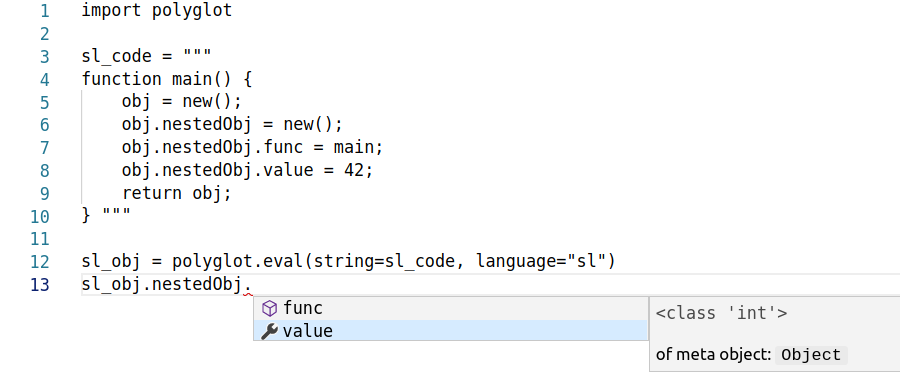
\includegraphics[width=\linewidth]{images/xp_report/completion_properties_polylgot.png}
  \caption[Polyglot code completion of properties]{\DIFaddFL{Completion of properties for a foreign \acs{sl} object in Python source code.}}
  \label{fig:xp:completionPolyglot}
\end{figure}

\subsection[]{\DIFadd{Application to Other Languages}}
\label{cha:evaluation}

\DIFadd{In this section}\DIFaddend , we show by means of the Truffle language implementations
Python, \DIFdelbegin \DIFdel{SimpleLanguage, }\DIFdelend FastR, and GraalSqueak that basic support of some \ac{lsp} features can
be achieved with minimal implementation effort \DIFaddbegin \DIFadd{in real languages}\DIFaddend . Furthermore,
we explain \DIFdelbegin \DIFdel{, why certain }\DIFdelend \DIFaddbegin \DIFadd{which }\DIFaddend \ac{lsp} features cannot be easily supported in some language
implementations \DIFdelbegin \DIFdel{. Finally, we describe }\DIFdelend \DIFaddbegin \DIFadd{and other }\DIFaddend limitations of our approach\DIFdelbegin \DIFdel{and implementation of }%DIFDELCMD < \graallsp%%%
\DIFdelend .

\DIFdelbegin \subsection[]{\DIFdel{Evaluated Truffle Languages}}
%DIFAUXCMD
\addtocounter{subsection}{-1}%DIFAUXCMD
\DIFdelend \DIFaddbegin \paragraph{\DIFadd{Evaluated Truffle Languages}}
\DIFaddend \label{sec:xp:ComparisonOfLangImpls}

\DIFdelbegin \DIFdel{\mbox{%DIFAUXCMD
\acf{sl}}\hspace{0pt}%DIFAUXCMD
}\footnote{%DIFDELCMD < \url{https://github.com/graalvm/simplelanguage} %%%
\DIFdel{(accessed
  2018-12-17)}} %DIFAUXCMD
\addtocounter{footnote}{-1}%DIFAUXCMD
\DIFdel{is Truffle's exemplary language implementation, to showcase
Truffle features and help understanding its ideas and concepts. \mbox{%DIFAUXCMD
\ac{sl} }\hspace{0pt}%DIFAUXCMD
has
first class functions. The type system only consists of primitive types and a
single }%DIFDELCMD < \inlinecode{object} %%%
\DIFdel{type. Objects are implemented as simple key-value
stores. As showcase implementation , it implements most of the needed Truffle
\mbox{%DIFAUXCMD
\acp{api} }\hspace{0pt}%DIFAUXCMD
so that, after implementing our proposed extensions with minimal
effort, \mbox{%DIFAUXCMD
\ac{sl} }\hspace{0pt}%DIFAUXCMD
supports nearly all }%DIFDELCMD < \graallsp%%%
\DIFdel{~features. }%DIFDELCMD < 

%DIFDELCMD < %%%
\DIFdelend \DIFaddbegin \DIFadd{The Python implementation for
GraalVM}\footnote{\url{https://github.com/graalvm/graalpython} \DIFadd{(accessed
  2018-12-17)}} \DIFadd{was modified to implement all }\api \DIFadd{we proposed. For
}\DIFaddend FastR\footnote{\url{https://github.com/oracle/fastr} (accessed 2018-12-17)}\DIFdelbegin \DIFdel{is a
high-performance }\DIFdelend \DIFaddbegin \DIFadd{, the
}\DIFaddend implementation of the R\footnote{\url{https://www.r-project.org} (accessed
  2018-12-17)} \DIFdelbegin \DIFdel{programming
languageused for statistical computing and graphics. Its goal is to become a
drop-in replacement for the reference implementation GNU-R. Due to time
constraints}\DIFdelend \DIFaddbegin \DIFadd{language}\DIFaddend , we have only implemented support for completion trigger
characters\DIFdelbegin \DIFdel{yet, so that the FastR }\DIFdelend \DIFaddbegin \DIFadd{, so the }\DIFaddend implementation is nearly unchanged. \DIFdelbegin \DIFdel{Therefore, not many
}%DIFDELCMD < \graallsp%%%
\DIFdel{~features are supported.
}%DIFDELCMD < 

%DIFDELCMD < %%%
\DIFdel{The Python implementation for
GraalVM}\footnote{%DIFDELCMD < \url{https://github.com/graalvm/graalpython} %%%
\DIFdel{(accessed
  2018-12-17)}} %DIFAUXCMD
\addtocounter{footnote}{-1}%DIFAUXCMD
\DIFdel{is less complete than R and does not support many libraries yet,
but is mature enough to demonstrate our approach. }%DIFDELCMD < 

%DIFDELCMD < %%%
\DIFdelend \DIFaddbegin \DIFadd{This demonstrates that we
can provide some support even with the least amount of language developer
effort. }\DIFaddend GraalSqueak~\cite{niephaus2018graalsqueak}\DIFdelbegin \DIFdel{is an early-stage experimental
}\DIFdelend \DIFaddbegin \DIFadd{, a }\DIFaddend Squeak/Smalltalk
\cite{ingalls1997back} implementation\DIFdelbegin \DIFdel{. In contrast to the other
selected languages, it is an image-based, graphical live-programming
environment. Furthermore, it uses the \mbox{%DIFAUXCMD
\ac{ast}}\hspace{0pt}%DIFAUXCMD
-based Truffle framework to
implement a bytecode interpreter}\DIFdelend \DIFaddbegin \DIFadd{, is image- rather than file-based and
executes bytecodes rather than a Smalltalk \mbox{%DIFAUXCMD
\ac{ast}}\hspace{0pt}%DIFAUXCMD
}\DIFaddend . Therefore, it is difficult
to map concepts of GraalSqueak to \DIFdelbegin \DIFdel{the file-based \mbox{%DIFAUXCMD
\ac{lsp}}\hspace{0pt}%DIFAUXCMD
protocol. Nonetheless, we }\DIFdelend \DIFaddbegin \DIFadd{\mbox{%DIFAUXCMD
\ac{lsp}}\hspace{0pt}%DIFAUXCMD
. We }\DIFaddend have chosen it to show that at
least some features can be supported with reasonable effort\DIFdelbegin \DIFdel{and
to discuss limitations of our approach. We run GraalSqueak in headless mode to
load an image and get access to its run-time objects. For now, we }\DIFdelend \DIFaddbegin \DIFadd{. We }\DIFaddend treat every
opened \inlinecode{st} file as an isolated Squeak/Smalltalk \DIFdelbegin \DIFdel{workspace.
}%DIFDELCMD < 

%DIFDELCMD < %%%
%DIF <  For SL, the implemented extensions are already available as public GitHub pull
%DIF <  requests. For GraalPython, FastR, and GraalSqueak, we implemented ... \todo{}
%DIFDELCMD < 

%DIFDELCMD < %%%
%DIF <  \autoref{tab:truffleAPIXLanguageMatrix} gives an overview over the status quo of
%DIF <  implemented Truffle \acp{api} of these languages. Futhermore,
%DIFDELCMD < \autoref{tab:lspFeatureXLanguageMatrix} %%%
\DIFdel{gives a broad overview over the
}%DIFDELCMD < \graallsp%%%
\DIFdel{~features supported by these languages. In the following, we will
highlight how well some of these features are already supported by showing and
describing screenshots of the usage in a language client. We use Visual Studio
Code to connect to an already running }%DIFDELCMD < \graallsp%%%
\DIFdel{~instance}\DIFdelend \DIFaddbegin \DIFadd{scope}\DIFaddend .

\DIFdelbegin %DIFDELCMD < \newcommand{\cmark}{\ding{51}}
%DIFDELCMD < \newcommand{\xmark}{\ding{55}}
%DIFDELCMD < \newcommand{\nyi}{\xmark}
%DIFDELCMD < 

%DIFDELCMD < %%%
\DIFdelend % \begin{table*}
%     \centering
%     \tableinsidecommand
%     \begin{threeparttable}
%       \caption[Language overview of supported Truffle \acp{api}]{An overview over selected Truffle languages and their current support of existing Truffle \acp{api} and our proposed extensions. Adjusting and extending these language implementations for \graallsp~is still work in progress, especially for FastR and GraalSqueak.}
%       \label{tab:truffleAPIXLanguageMatrix}
%       \begin{tabular}{ l c c c c }
%         \toprule
%DIF <          Truffle \ac{api} (existing and extensions)     & SL & GraalPython & FastR & GraalSqueak \\
%DIF >          Truffle \ac{api} (existing and extensions)     & \ac{SL} & GraalPython & FastR & GraalSqueak \\
%         \midrule
%         CallTag                                         & \cmark & \cmark & \cmark & \xmark \\
%         StatementTag                                    & \cmark & \cmark & \cmark & \cmark \\
%         ExpressionTag                                   & \cmark & \cmark & \nyi & \nyi \\
%         findTopScopes()                                 & \cmark & \cmark & \cmark & \cmark \\
%         findLocalScopes()                               & \cmark & \cmark & \cmark\tnote{r} & \nyi \\
%         findMetaObject()                                & \cmark\tnote{n} & \cmark & \cmark\tnote{n} & \cmark \\
%         findSourceLocation()                            & \cmark & \cmark & \cmark & \nyi\tnote{?} \\
%         parse() eager \ac{ast} creation                 & \cmark & \cmark & \cmark & \xmark \\
%         parseInline()                                   & \xmark & \cmark & \cmark & \nyi \\
%         \midrule
%         getCompletionTriggerCharacters()                & \cmark & \cmark & \cmark & \cmark \\
%         getSignatureHelpTriggerCharacters()             & \nyi & \cmark & \nyi & \nyi \\
%         getNodeObject() for literal nodes               & \cmark & \cmark & \nyi & \nyi \\
%         boxPrimitive()                                  & \xmark & \cmark & \nyi & \nyi \\
%         GetSignature custom message                     & \xmark & \cmark & \nyi & \nyi \\
%         GetDocumentation custom message                 & \xmark & \cmark & \nyi & \nyi \\
%         DeclarationTag, Read/WriteVariableTag           & \cmark & \cmark & \nyi & \nyi \\
%         \bottomrule
%       \end{tabular}
%       \begin{tablenotes}
%         \item [r] Run-time scopes only
%         \item [n] Names of meta-objects only
%         \item [?] Unclear how to implement
%       \end{tablenotes}
%     \end{threeparttable}
% \end{table*}

\DIFdelbegin %DIFDELCMD < \begin{table*}
%DIFDELCMD <   \small
%DIFDELCMD <     \centering
%DIFDELCMD <     \tableinsidecommand
%DIFDELCMD <     \begin{threeparttable}
%DIFDELCMD <       %%%
%DIFDELCMD < \caption[Language overview of supported \graallsp~features]{%
{%DIFAUXCMD
\DIFdelFL{An overview over selected Truffle languages and their support of }%DIFDELCMD < \graallsp%%%
\DIFdelFL{~features. %DIF <  If a feature is not supported, it will either depend on not yet implemented Truffle \acp{api} as described in \autoref{tab:truffleAPIXLanguageMatrix}, or on missing information due to a run-time focused language implementation.
      }}
      %DIFAUXCMD
%DIFDELCMD < \label{tab:lspFeatureXLanguageMatrix}
%DIFDELCMD <       \begin{tabular}{ l c c c c }
%DIFDELCMD <         \toprule
%DIFDELCMD <         %%%
\DIFdelFL{\mbox{%DIFAUXCMD
\ac{lsp} }\hspace{0pt}%DIFAUXCMD
feature }%DIFDELCMD < & %%%
\DIFdelFL{SL }%DIFDELCMD < & %%%
\DIFdelFL{GraalPython }%DIFDELCMD < & %%%
\DIFdelFL{FastR}%DIFDELCMD < & %%%
\DIFdelFL{GraalSqueak}%DIFDELCMD < \\
%DIFDELCMD <         \midrule
%DIFDELCMD <         %%%
\DIFdelFL{Diagnostics             }%DIFDELCMD < & \cmark & \cmark & \xmark & \cmark \\
%DIFDELCMD <         %%%
\DIFdelFL{Completion (globals)    }%DIFDELCMD < & \cmark & \cmark & \cmark & \cmark \\
%DIFDELCMD <         %%%
\DIFdelFL{Completion (locals)     }%DIFDELCMD < & \cmark & \cmark & \cmark\tnote{*} & \xmark \\
%DIFDELCMD <         %%%
\DIFdelFL{Completion (properties) }%DIFDELCMD < & \cmark\tnote{*} & \cmark\tnote{*} & \xmark & \xmark \\
%DIFDELCMD <         %%%
\DIFdelFL{Signature Help          }%DIFDELCMD < & \xmark & \cmark\tnote{*} & \xmark & \xmark \\
%DIFDELCMD <         %%%
\DIFdelFL{Hover                   }%DIFDELCMD < & \cmark\tnote{*} & \cmark\tnote{*} & \cmark\tnote{*} & \xmark \\
%DIFDELCMD <         %%%
\DIFdelFL{Symbols                 }%DIFDELCMD < & \cmark & \cmark & \cmark & \xmark \\
%DIFDELCMD <         %%%
\DIFdelFL{Goto-definition (callables)              }%DIFDELCMD < & \cmark\tnote{*} & \cmark\tnote{*} & \cmark\tnote{*} & \xmark\tnote{?}  \\
%DIFDELCMD <         %%%
\DIFdelFL{Goto-definition (local variables)              }%DIFDELCMD < & \cmark & \cmark & \xmark & \xmark \\
%DIFDELCMD <         %%%
\DIFdelFL{References (static)     }%DIFDELCMD < & \cmark & \cmark & \xmark & \xmark\tnote{?} \\
%DIFDELCMD <         %%%
\DIFdelFL{Highlighting variables  }%DIFDELCMD < & \cmark & \cmark & \xmark & \xmark \\
%DIFDELCMD <         \bottomrule
%DIFDELCMD <       \end{tabular}
%DIFDELCMD <       \begin{tablenotes}
%DIFDELCMD <         \item [%%%
\DIFdelFL{*}%DIFDELCMD < ] %%%
\DIFdelFL{Requires run-time information
        }%DIFDELCMD < \item [%%%
\DIFdelFL{?}%DIFDELCMD < ] %%%
\DIFdelFL{Unclear }\DIFdelendFL \DIFaddbeginFL \paragraph{\DIFaddFL{Navigational Features}}

\DIFaddFL{Both Python and FastR automatically support querying global symbols and
navigating to them. For Smalltalk, this feature is not available, because the
global symbols are not defined in any source file, but are part of the
image. Thus, while we can list global symbols, we cannot offer a source location
for them, which is required for the highlighting that \mbox{%DIFAUXCMD
\ac{lsp} }\hspace{0pt}%DIFAUXCMD
clients want to
support, as seen in }\autoref{fig:xp:symbolsPython}\DIFaddFL{.
}

\begin{figure}
    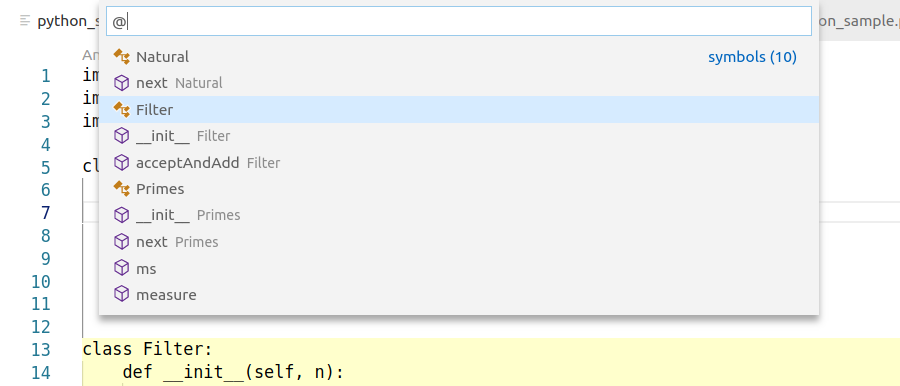
\includegraphics[width=\linewidth]{images/xp_report/symbols_Python.png}
    \caption{\DIFaddFL{Symbol overview over the current Python document. The selected entry's source section is highlighted in the editor.}}
    \label{fig:xp:symbolsPython}
\end{figure}

\DIFaddFL{To jump to definitions, we implemented the new DeclarationTag in Python to
support jumping to the definition of local variables. For FastR, we did not
change anything, but since the language supports returning the source location
for functions, jumping to the definition of functions when runtime information
is available worked immediately. In GraalSqueak, the DeclarationTag could enable
jumping to the definition of local variables, but it's unclear }\DIFaddendFL how to implement
\DIFdelbeginFL %DIFDELCMD < \end{tablenotes}
%DIFDELCMD <     \end{threeparttable}
%DIFDELCMD < \end{table*}
%DIFDELCMD < %%%
\DIFdelend \DIFaddbegin \DIFadd{jumping to function definitions at all. Futhermore, GraalSqueak works on
bytecode, yet in Smalltalk source code, variables are declared explicitly at the
beginning of blocks or methods. These declarations, however, are not available
in the bytecode, where variables are only referenced by index. Thus, the
Smalltalk implementation would have to do significant work to map back from
\mbox{%DIFAUXCMD
\ac{ast} }\hspace{0pt}%DIFAUXCMD
nodes representing bytecode locations to source locations.
}

\DIFadd{To fully support references, we had to add Write- and ReadVariableTags to
Python. While FastR uses the CallTag, and thus we can provide references and
highlights for functions, we cannot do the same for local
variables. Additionally, scoping information in R relies on the dynamic
execution extent, and thus we cannot properly support these features on FastR
without both the tags and runtime information.
}

\paragraph{\DIFadd{Informational Features}}
\DIFaddend 

\DIFdelbegin \subparagraph{\DIFdel{Diagnostics}} %DIFAUXCMD
\addtocounter{subparagraph}{-1}%DIFAUXCMD
\DIFdelend All languages except FastR fail parsing at the first syntax error, so that only
one error per file can be sent to the client. \DIFdelbegin %DIFDELCMD < \autoref{fig:xp:diagnosticsSL} %%%
\DIFdel{displays how such a diagnostics
notification is visualized in \mbox{%DIFAUXCMD
\ac{sl}}\hspace{0pt}%DIFAUXCMD
. }\DIFdelend FastR does not throw a
\inlinecode{TruffleException} in case of a syntax error, so that
\graallsp~cannot report any syntax errors for FastR. %DIF < GraalSqueak does not support eager parsing yet, so that we have to execute the code to trigger the actual parsing. Then, the first syntax error is reported via a \inlinecode{TruffleException}.
\DIFaddbegin \DIFadd{However, this is arguably a
bug in the FastR implementation, as it also affects other tools such as the
debugger.
}

\DIFadd{Signature help and documentation requests are only fully implemented in
Python. These use our newly introduced GetSignature and GetDocumentation
messages. In Python, these were easy to implement since functions already store
and expose their documentation to user code
(}\autoref{fig:xp:signatureHelpPython}\DIFadd{). For the implementation of these messages
we thus just had to map them to the appropriate Python code. For Smalltalk
classes and functions, we implemented the GetDocumentation message to show the
last modified date, category, and author; these are stored as meta-data on these
Smalltalk objects anyway.
}\DIFaddend 

\begin{figure}
    \DIFdelbeginFL %DIFDELCMD < 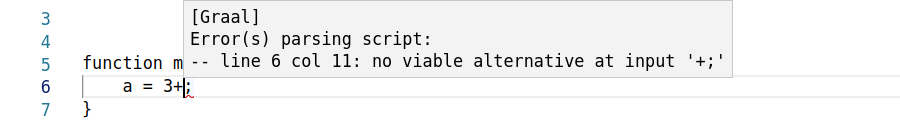
\includegraphics[width=\linewidth]{images/xp_report/diagnostics_sl.png}
%DIFDELCMD <     \caption[Diagnostics used to display a syntax error in \acs{sl}]{%%%
\DIFdelFL{Diagnostics used to display a syntax error in \acs{sl}}\DIFdelendFL \DIFaddbeginFL 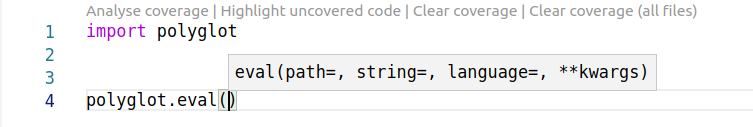
\includegraphics[width=\linewidth]{images/xp_report/signature_help_python.png}
    \caption{\DIFaddFL{Signature help for Python}\DIFaddendFL .}
    \DIFdelbeginFL %DIFDELCMD < \label{fig:xp:diagnosticsSL}
%DIFDELCMD < %%%
\DIFdelendFL \DIFaddbeginFL \label{fig:xp:signatureHelpPython}
\DIFaddendFL \end{figure}

\DIFdelbegin \subparagraph{\DIFdel{Code Completion}} %DIFAUXCMD
\addtocounter{subparagraph}{-1}%DIFAUXCMD
\DIFdelend \DIFaddbegin \DIFadd{Finally, hover information is available to the same extent as for \mbox{%DIFAUXCMD
\ac{sl} }\hspace{0pt}%DIFAUXCMD
in all
three other languages, since they each support dynamic evaluation of source code
in a given runtime frame. An example for FastR is shown in
}\autoref{fig:xp:hoverR}\DIFadd{.
}

\begin{figure}
    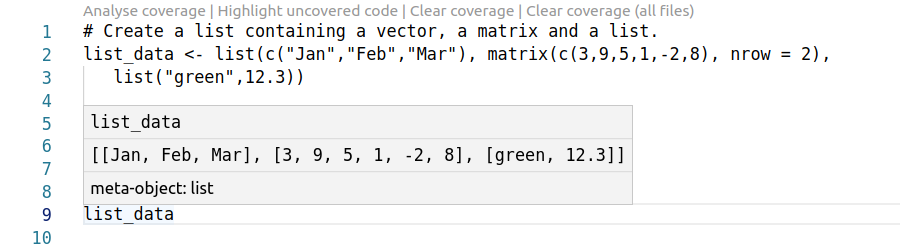
\includegraphics[width=\linewidth]{images/xp_report/hover_R.png}
    \caption[Hover information in FastR source code]{\DIFaddFL{Displaying information on mouse hover for FastR source code using cached run-time information.}}
    \label{fig:xp:hoverR}
\end{figure}

%DIF >  \paragraph{Renaming} Since only GraalPython supports finding the exact
%DIF >  definition location of a callable and finding its references, renaming only
%DIF >  works for that language in addition to \ac{sl}.

\paragraph{\DIFadd{Completion}}

\DIFaddend \autoref{fig:xp:completionGlobalsPython} shows a code completion for globals and
locals in \DIFdelbegin \DIFdel{GraalPython}\DIFdelend \DIFaddbegin \DIFadd{Python}\DIFaddend . Completion items have different icons for classes, methods,
and variables in the list of suggestions. For the selected item of a built-in
class, a string representation of the corresponding meta-object is displayed,
together with a documentation, if available. The same support is available \DIFdelbegin \DIFdel{in \mbox{%DIFAUXCMD
\ac{sl} }\hspace{0pt}%DIFAUXCMD
(which can lexically provide
local scopes), FastR (which needs run-time information for
locals), }\DIFdelend \DIFaddbegin \DIFadd{for
FastR %DIF >  (using runtime information for local scopes,
%DIF >  \autoref{fig:xp:completionGlobalsR}), 
}\DIFaddend and GraalSqueak
(\DIFdelbegin \DIFdel{which only shows the globals available in the Smalltalk
dictionary}\DIFdelend \DIFaddbegin \autoref{fig:xp:completionGlobalsGraalSqueak}\DIFaddend ).

%DIF <  \autoref{fig:xp:completionLocalsSL} shows a code completion in
%DIF <  \ac{sl}. Variables of lexical local scopes are listed first, followed by
%DIF <  built-in functions. For the selected local variable, the scope name is
%DIF <  displayed. \autoref{fig:xp:completionGlobalsR} shows a completion of globals in
%DIF <  FastR, with an already filtered list of globals containing the string
%DIF <  \inlinecode{"as"}. The completion of locals in FastR is supported only if
%DIF <  run-time information, i.e. a frame, is
%DIF <  available. \autoref{fig:xp:completionGlobalsGraalSqueak} shows globals of the
%DIF <  Smalltalk dictionary for GraalSqueak.
\DIFdelbegin %DIFDELCMD < 

%DIFDELCMD < %%%
\DIFdelend \begin{figure}
    \DIFdelbeginFL %DIFDELCMD < 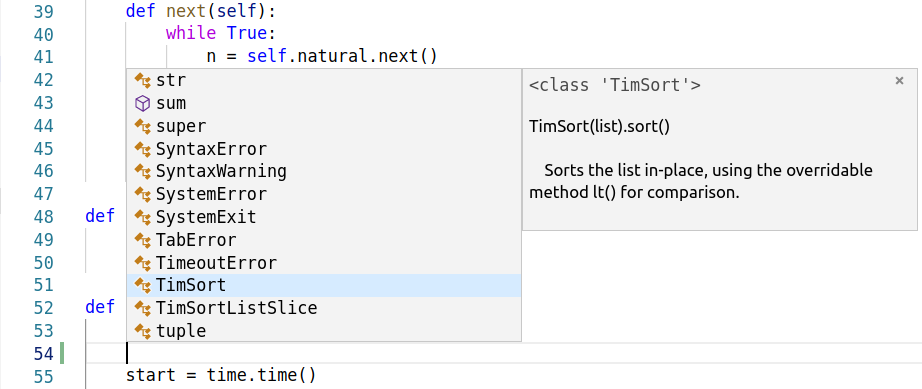
\includegraphics[width=\linewidth]{images/xp_report/code_completion_globals_python_with_docu.png}
%DIFDELCMD <     \caption[Code completion of globals and locals in GraalPython]{%%%
\DIFdelFL{Code completion }\DIFdelendFL \DIFaddbeginFL 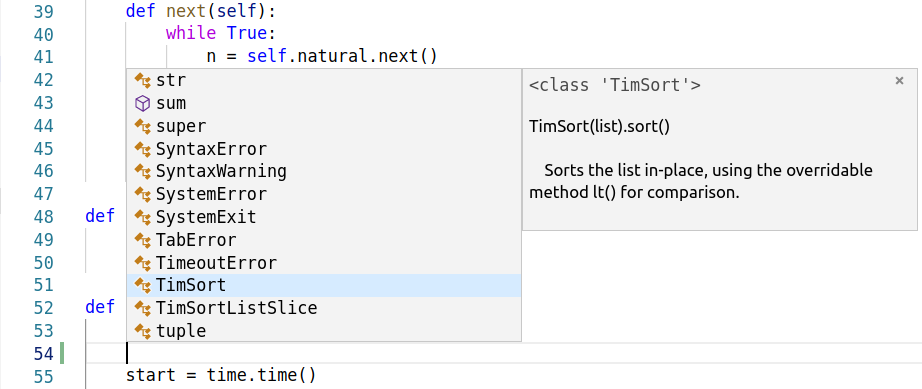
\includegraphics[width=0.8\linewidth]{images/xp_report/code_completion_globals_python_with_docu.png}
    \caption{\DIFaddFL{Completion }\DIFaddendFL of globals \DIFdelbeginFL \DIFdelFL{and locals }\DIFdelendFL \DIFaddbeginFL \DIFaddFL{with documentation }\DIFaddendFL in \DIFdelbeginFL \DIFdelFL{GraalPython}\DIFdelendFL \DIFaddbeginFL \DIFaddFL{Python}\DIFaddendFL .}
    \label{fig:xp:completionGlobalsPython}
\end{figure}

% \begin{figure}
%DIF <      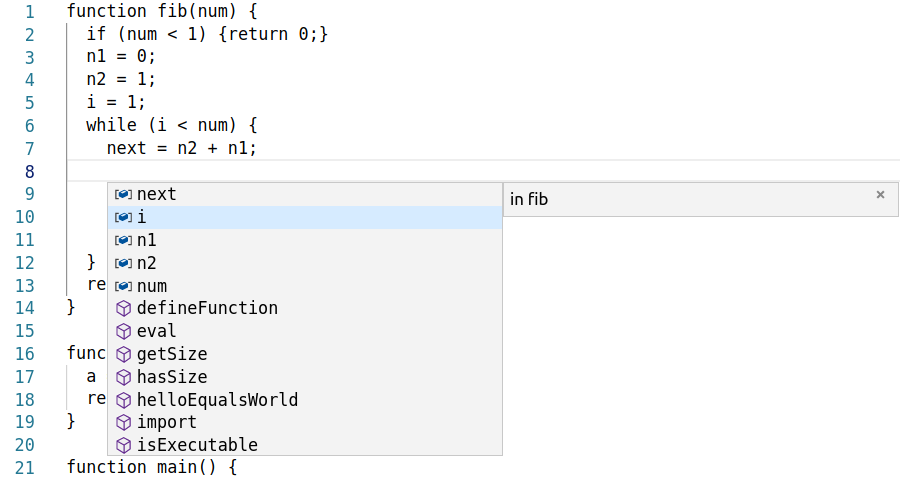
\includegraphics[width=\linewidth]{images/xp_report/code_completion_locals_sl.png}
%DIF <      \caption[Code completion of globals and locals in \acs{sl}]{Code completion of globals and locals in \acs{sl}.}
%DIF <      \label{fig:xp:completionLocalsSL}
%DIF <  \end{figure}
\DIFdelbegin %DIFDELCMD < 

%DIFDELCMD < %%%
%DIF <  \begin{figure}
%DIF <      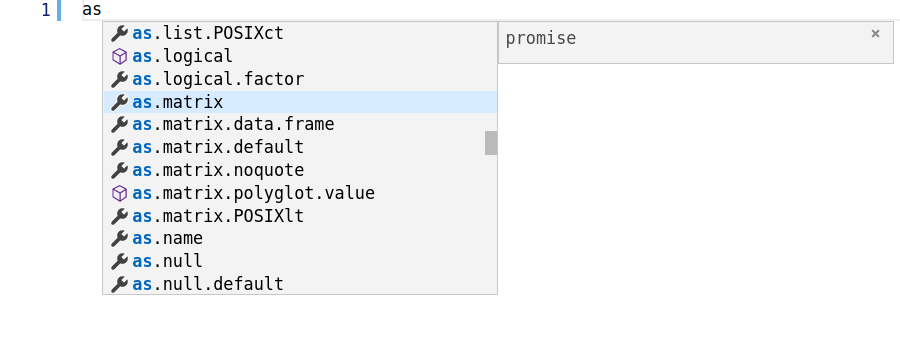
\includegraphics[width=\linewidth]{images/xp_report/code_completion_globals_R.png}
\DIFdelend %DIF >      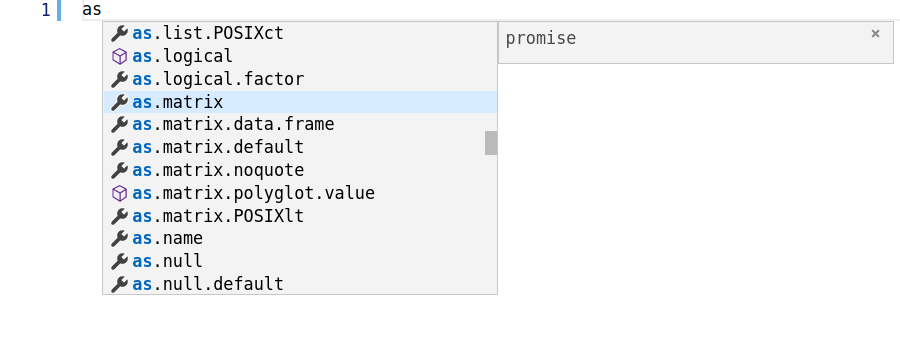
\includegraphics[width=0.8\linewidth]{images/xp_report/code_completion_globals_R.png}
%     \caption[Code completion of globals in FastR]{Code completion of globals in FastR.}
%     \label{fig:xp:completionGlobalsR}
% \end{figure}

%DIF <  \begin{figure}
%DIF <      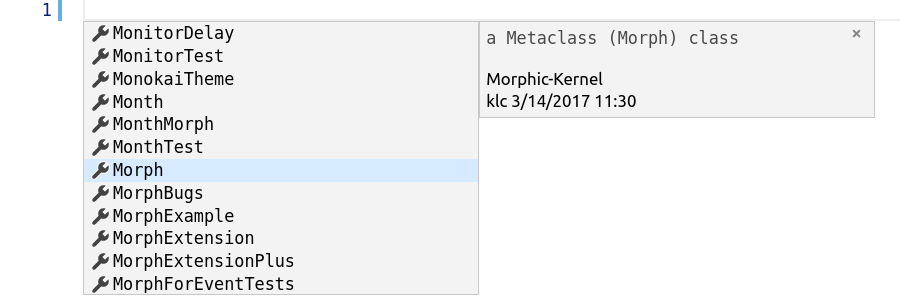
\includegraphics[width=\linewidth]{images/xp_report/code_completion_globals_GraalSqueak.png}
%DIF <      \caption[Code completion of globals in GraalSqueak]{Code completion of globals in GraalSqueak.}
%DIF <      \label{fig:xp:completionGlobalsGraalSqueak}
%DIF <  \end{figure}
\DIFaddbegin \begin{figure}
    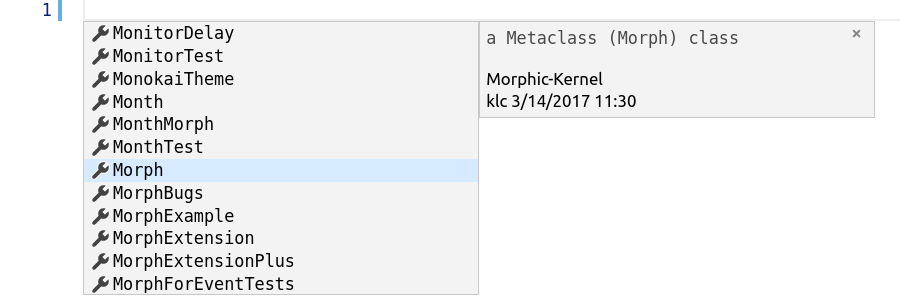
\includegraphics[width=0.8\linewidth]{images/xp_report/code_completion_globals_GraalSqueak.png}
    \caption[Code completion of globals in GraalSqueak]{\DIFaddFL{Code completion of globals in GraalSqueak.}}
    \label{fig:xp:completionGlobalsGraalSqueak}
\end{figure}
\DIFaddend 

The code completion of properties is supported to different extents in these
languages. Run-time information are always required due to the dynamic nature of
the languages. \DIFdelbegin \DIFdel{Therefore, the source code needs to be parsable after removing
the trigger character. For \mbox{%DIFAUXCMD
\ac{sl}}\hspace{0pt}%DIFAUXCMD
, }%DIFDELCMD < \graallsp%%%
\DIFdel{~supports the completion of
properties, which are the keys of the underlying key-value store. For
GraalPython, properties of objects can also be those inherited from their type
hierarchy including fields and methods of their classes. }\DIFdelend For FastR and GraalSqueak, we were not able to provide a
completion of properties yet, although the Truffle \DIFdelbegin \DIFdel{\mbox{%DIFAUXCMD
\ac{api} }\hspace{0pt}%DIFAUXCMD
}\DIFdelend \DIFaddbegin \api \DIFaddend allows it. These
languages are missing an expression annotation on their \ac{ast}
nodes. \DIFdelbegin \DIFdel{In GraalPython}\DIFdelend \DIFaddbegin \DIFadd{Implementing it will not only help the \mbox{%DIFAUXCMD
\ac{lsp} }\hspace{0pt}%DIFAUXCMD
support, but also add
support for column breakpoints in the Chrome debugger, for example.
}

\DIFadd{In Python}\DIFaddend , triggering a completion of properties for the code snippet
\inlinecode{anObject.nestedObject}, by inserting a dot at the end, will yield
completion items for all properties of the object referenced by
\inlinecode{anObject.nestedObject}, because the nearest node tagged as
expression is the one representing the whole source section. In \ac{sl},
however, inserting a dot before the semicolon in \DIFaddbegin \DIFadd{the expressoin
}\DIFaddend \inlinecode{anObject.nestedObject;} to trigger code completion, will yield no
results, because the nearest node tagged as expression represents just the
\inlinecode{nestedObject} string, and not
\inlinecode{anObject.nestedObject}. This highlights that the developer has to
take a bit of care designing their \ac{ast} for optimal developer experience.

\DIFdelbegin \DIFdel{Using GraalPython and \mbox{%DIFAUXCMD
\ac{sl}}\hspace{0pt}%DIFAUXCMD
, we want to highlight, that Truffle supports
polyglot programming and we can therefore provide completion of properties
across language boundaries. }%DIFDELCMD < \autoref{fig:xp:completionPolyglot} %%%
\DIFdel{shows Python
code evaluating a \mbox{%DIFAUXCMD
\ac{sl} }\hspace{0pt}%DIFAUXCMD
code snippet which creates and returns a \mbox{%DIFAUXCMD
\ac{sl}
}\hspace{0pt}%DIFAUXCMD
object. In the last line, we get completions of properties for the foreign
\mbox{%DIFAUXCMD
\ac{sl} }\hspace{0pt}%DIFAUXCMD
object, which would not be possible in \mbox{%DIFAUXCMD
\ac{sl} }\hspace{0pt}%DIFAUXCMD
code, as described in the
previous paragraph.
}%DIFDELCMD < 

%DIFDELCMD < %%%
\DIFdel{The code completion request for properties is triggered fairly often in
comparison to the other run-time information requiring requests. Unfortunately,
the performance depends on the one hand on the execution time of the source
code, which can be reduced by caching run-time information, but on the other
hand it depends on the creation time of Truffle language contexts. We create a
new one for each execution, which is quite cheap for \mbox{%DIFAUXCMD
\ac{sl}}\hspace{0pt}%DIFAUXCMD
, but for
GraalPython, it takes a noticeable time. Reusing those contexts improves the
performance, but introduces problems with cache invalidation and memory usage.
}%DIFDELCMD < 

%DIFDELCMD < \begin{figure}
%DIFDELCMD <     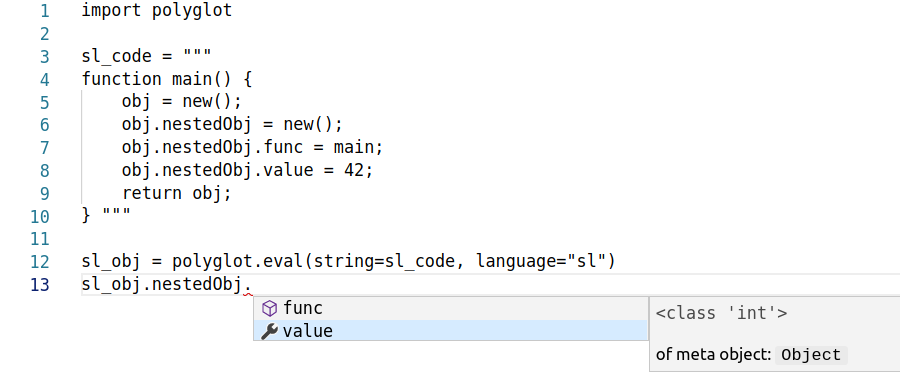
\includegraphics[width=\linewidth]{images/xp_report/completion_properties_polylgot.png}
%DIFDELCMD <     %%%
%DIFDELCMD < \caption[Polyglot code completion of properties]{%
{%DIFAUXCMD
\DIFdelFL{Completion of properties for a foreign \acs{sl} object in GraalPython source code.}}
    %DIFAUXCMD
%DIFDELCMD < \label{fig:xp:completionPolyglot}
%DIFDELCMD < \end{figure}
%DIFDELCMD < 

%DIFDELCMD < %%%
\subparagraph{\DIFdel{Signature Help}} %DIFAUXCMD
\addtocounter{subparagraph}{-1}%DIFAUXCMD
\DIFdel{Signature help is only supported with our proposed
additional \mbox{%DIFAUXCMD
\ac{api}}\hspace{0pt}%DIFAUXCMD
, which we implemented for Python. }%DIFDELCMD < \graallsp%%%
\DIFdel{~can provide a
formatted signature string as shown in
}%DIFDELCMD < \autoref{fig:xp:signatureHelpPython}%%%
\DIFdel{. Implementing this message for example in
\mbox{%DIFAUXCMD
\ac{sl} }\hspace{0pt}%DIFAUXCMD
might not be possible without changes to the language, because \mbox{%DIFAUXCMD
\ac{sl}
}\hspace{0pt}%DIFAUXCMD
stores function arguments internally like any other local variable of the
function, so that there is no knowledge left at run-time to obtain the signature
of a function. This is an example where language developers need to store
additional parse-time information to support more \mbox{%DIFAUXCMD
\ac{lsp} }\hspace{0pt}%DIFAUXCMD
features.
}%DIFDELCMD < 

%DIFDELCMD < \begin{figure}
%DIFDELCMD <     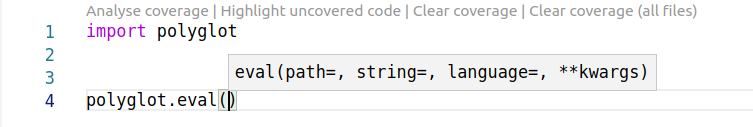
\includegraphics[width=\linewidth]{images/xp_report/signature_help_python.png}
%DIFDELCMD <     %%%
%DIFDELCMD < \caption[Signature help for GraalPython]{%
{%DIFAUXCMD
\DIFdelFL{Signature help for GraalPython.}}
    %DIFAUXCMD
%DIFDELCMD < \label{fig:xp:signatureHelpPython}
%DIFDELCMD < \end{figure}
%DIFDELCMD < 

%DIFDELCMD < %%%
\subparagraph{\DIFdel{Hover}}
%DIFAUXCMD
\addtocounter{subparagraph}{-1}%DIFAUXCMD
\DIFdel{Showing information on mouse hover is supported for variables and expressions of \mbox{%DIFAUXCMD
\ac{sl} }\hspace{0pt}%DIFAUXCMD
and GraalPython yet. For FastR, only variables can be accessed via their corresponding frame slot, to provide hover information. For all languages, cached run-time information needs to be available. A collection run can be triggered using the }\emph{\DIFdel{codeLens}} %DIFAUXCMD
\DIFdel{named }\emph{\DIFdel{Analyse coverage}}%DIFAUXCMD
\DIFdel{, as shown above the first line of code in }%DIFDELCMD < \autoref{fig:xp:hoverR}%%%
\DIFdel{. The displayed hover information includes a string representation of the variable's value and the meta-object.
}%DIFDELCMD < 

%DIFDELCMD < \begin{figure}
%DIFDELCMD <     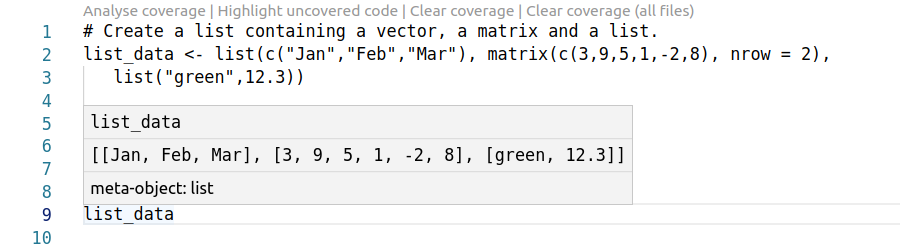
\includegraphics[width=\linewidth]{images/xp_report/hover_R.png}
%DIFDELCMD <     %%%
%DIFDELCMD < \caption[Hover information in FastR source code]{%
{%DIFAUXCMD
\DIFdelFL{Displaying information on mouse hover for FastR source code using cached run-time information.}}
    %DIFAUXCMD
%DIFDELCMD < \label{fig:xp:hoverR}
%DIFDELCMD < \end{figure}
%DIFDELCMD < 

%DIFDELCMD < %%%
\subparagraph{\DIFdel{Symbols}} %DIFAUXCMD
\addtocounter{subparagraph}{-1}%DIFAUXCMD
\DIFdel{As soon as a language eagerly creates \mbox{%DIFAUXCMD
\ac{ast} }\hspace{0pt}%DIFAUXCMD
nodes when
the source code is parsed, }%DIFDELCMD < \graallsp%%%
\DIFdel{~can support the request for symbols by
providing the names of all function root node instances known to the
framework. Nodes can further be annotated as declarations, which we can use to
choose symbol type and container name as shown for GraalPython in
}%DIFDELCMD < \autoref{fig:xp:symbolsPython}%%%
\DIFdel{.
}%DIFDELCMD < 

%DIFDELCMD < \begin{figure}
%DIFDELCMD <     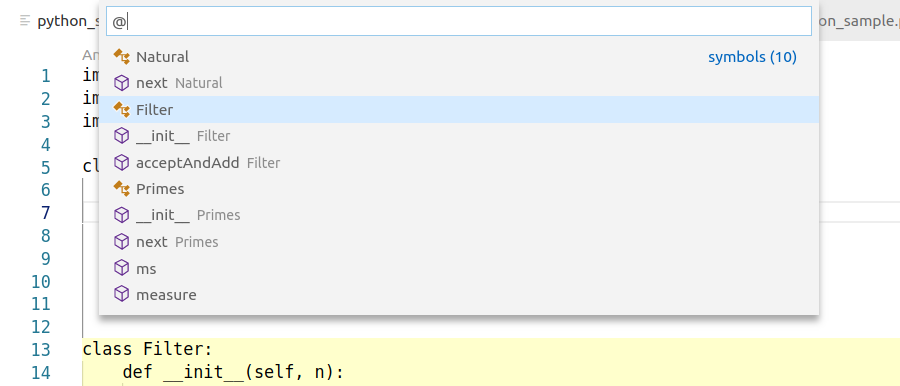
\includegraphics[width=\linewidth]{images/xp_report/symbols_Python.png}
%DIFDELCMD <     %%%
%DIFDELCMD < \caption[Symbol overview in GraalPython]{%
{%DIFAUXCMD
\DIFdelFL{Symbol overview over the current GraalPython document. The selected entry's source section is highlighted in the editor.}}
    %DIFAUXCMD
%DIFDELCMD < \label{fig:xp:symbolsPython}
%DIFDELCMD < \end{figure}
%DIFDELCMD < 

%DIFDELCMD < %%%
\subparagraph{\DIFdel{Goto-definition and References}}
%DIFAUXCMD
\addtocounter{subparagraph}{-1}%DIFAUXCMD
%DIF < Our Goto-definition implementation for callables might behave a bit unexpected for languages having first class functions like GraalPython or \ac{sl}. It is not always obvious, if a goto-definition request targets the variable which is read to get the callable object, or the callable itself. For example, for GraalPython  \inlinecode{} . Additionally, the behavior of our implementation depends on the language support. If \inlinecode{ReadVariableTag} and \inlinecode{WriteVariableTag} are supported, we can differentiate between a jump to the variable definition and a jump to the callable definition. Otherwise we will always jump to the callable definition.
\DIFdel{Our goto-definition and find-all-references implementations depend on the
supported tags of the Truffle language. The selected languages use the annotate
nodes representing a call, so that goto-definition can be supported using
run-time information. This works also across language boundaries, when using
Truffle's polyglot \mbox{%DIFAUXCMD
\ac{api}}\hspace{0pt}%DIFAUXCMD
. Without run-time we can use a static symbol
search. For GraalSqueak, which is not file-based, we do not know yet what a
useful implementation of navigational requests might look like.
}%DIFDELCMD < 

%DIFDELCMD < %%%
\subparagraph{\DIFdel{Variable Highlighting}} %DIFAUXCMD
\addtocounter{subparagraph}{-1}%DIFAUXCMD
\DIFdel{To support highlighting of variable
accesses (}%DIFDELCMD < \autoref{fig:xp:highlightingPython}%%%
\DIFdel{) we use nodes tagged as variable
}\emph{\DIFdel{reads}} %DIFAUXCMD
\DIFdel{and }\emph{\DIFdel{writes}}%DIFAUXCMD
\DIFdel{. Here, the language developer needs to take care
of assigning the correct source sections to their nodes for the highlighting to
look correct. With correct assignments, we could also use these tags to support
the }\emph{\DIFdel{rename}} %DIFAUXCMD
\DIFdel{refactoring for local variables.
}%DIFDELCMD < 

%DIFDELCMD < \begin{figure}
%DIFDELCMD <     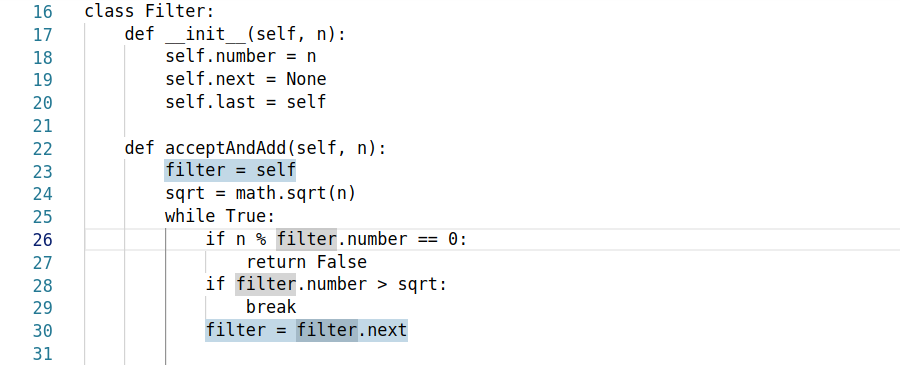
\includegraphics[width=\linewidth]{images/xp_report/highlighting_Python.png}
%DIFDELCMD <     %%%
%DIFDELCMD < \caption[Highlighting of variable accesses in GraalPython]{%
{%DIFAUXCMD
\DIFdelFL{Highlighting of variable accesses in GraalPython. The source sections of write accesses cover the whole assignment and are highlighted in a blueish shade.}}
    %DIFAUXCMD
%DIFDELCMD < \label{fig:xp:highlightingPython}
%DIFDELCMD < \end{figure}
%DIFDELCMD < 

%DIFDELCMD < %%%
%DIF <  \paragraph{GraalPython, SL, (Graal.js), FastR usage check}
%DIF <  \begin{itemize}
%DIF <      \item matrix of \graallsp~features x Truffle languages
%DIF <      \item list SLOC for adjustments of these langs
%DIF <      \item matrix of \graallsp~features x Truffle languages without language adjustments? Should be only completion of globals/locals and static stuff possible -> or add a footnote in the first matrix, to mark that it is only working with adjustments
%DIF <      \item include screenshots of VSCode for important LSP features, put rest in appendix?
%DIF <  \end{itemize}
%DIFDELCMD < 

%DIFDELCMD < %%%
%DIF <  \paragraph{other stuff}
%DIF <  \begin{itemize}
%DIF <      \item Completion response time
%DIF <      \item Eat your own dog food - Hover: We used the static hover information ourselves during implementation.
%DIF <      \item Between IDE and Language Workbench
%DIF <  \end{itemize}
    %DIFDELCMD < 

%DIFDELCMD < %%%
%DIF <  \paragraph{Between IDE and Language Workbench}
%DIF <      Language Workbench focus/aim: Efficient language (DSL) development, performance is not main focus
%DIF <      vs. Graal/Truffle aim: Efficient execution
%DIFDELCMD < 

%DIFDELCMD < %%%
%DIF <      Assumption: Language Workbenches use static information only, our Truffle-based solution uses dynamic type information
%DIFDELCMD < 

%DIFDELCMD < %%%
%DIF <  \subsection{Limitations of \graallsp}
%DIF <  \label{sec:xp:limitations}
%DIF <  \begin{itemize}
    %DIF < \item Server: Only TCP (connecting to already running server), no std-in/-out impl + typically a language server life cycle is controlled by the client (start+shutdown). Our impl started external.
    %DIF < \item Truffle: Only first syntax error is reported. Lang parsers fail on first error
    %DIF < \item Cancellation of requests not yet supported
    %DIF < \item also, this in-line eval is interpretation only
    %DIF < \item sandboxing limited to fie I/O + read-only FS atm
    %DIF < \item limitations due to caching of last nested context - show example of dirty context, e.g. function renamed
    %DIF < \item Using cached run-time infos: we have frame but to do in-line eval we call node.execute(frame) ourselves without having a valid execution stack there -> if the execution relies on the stack, it will not work
    %DIF < \item Context creation time expensive
    %DIF < \item performance
    %DIF < \item type harvesting: we take a snapshot of the frame for the first entering of a source section -> different types for a frame slot are ignored
    %DIF < \item memory consumption? We avoid GC of lots of objects by caching frames.
    %DIF < \item the snapshot taken copies frame and descriptor, but no deep copy of objects is done. Therefore the reference to these objects will represent the last state of execution
%DIFDELCMD < 

%DIFDELCMD <     %%%
%DIF < \item Graal compiler optimizations -> overhead for short scripts?!
    %DIF < \item typically one lang per server -> dynamic detection of languages + polyglot makes impl harder
    %DIF < \item example: Using R and Python -> R has dot in names of globals, for Python it is a trigger char -> dot char interrupts current completion, because a new one is triggered \autoref{fig:xp:completionGlobalsR}
    %DIFDELCMD < 

%DIFDELCMD <     %%%
%DIF <  \item \todo{open limitations}TruffleObject KEYS not hierarchical
    %DIF <  \item + no differentiation between properties of objects and methods of class
    %DIF <  \item Run-time type collection / type harvesting
    %DIF <  \begin{itemize}
    %DIF <      %\item caching is poorly conceived: storing frames / objects -> memory? + in-line eval without call stack difficult
    %DIF <      %\item framework needs to support instrumentation / tracing to find the desired run-time object
    %DIF <      %\item needs possibility to query the resulting host language object about its guest language semantics (e.g. a TruffleObject understanding a KEYS message)
    %DIF <      \item we query the actual run-time object, which might be really specialized, whereas type harvesting builds generalizations on seen types and yields only the generalized type
    %DIF <  \end{itemize}
    %DIF < \item code completion of properties only possible if dot is the last char inserted
%DIF <  \end{itemize}
%DIFDELCMD < 

%DIFDELCMD < %%%
%DIF <  Due to time constraints and limitations of the Truffle framework, we were unable
%DIF <  to fully implement the approach described in \autoref{cha:solution}. We have not
%DIF <  yet implemented a timeout or cancellation support for requests, to avoid an
%DIF <  endless execution of source code when collecting run-time information. The
%DIF <  suggested sandboxing of the execution engine is limited to file I/O for now,
%DIF <  because Truffle does not support restriction of other I/O kinds
%DIF <  yet. Furthermore, the sandbox is always activated when source code is executed,
%DIF <  because we have not yet implemented a possibility to deactivate sandboxing when
%DIF <  the user classifies the occurring side-effects as uncritical. Therefore, all
%DIF <  features of \graallsp, which require collecting run-time information, are not
%DIF <  supported yet, if the executed source code requires write access to the file
%DIF <  system. For GraalSqueak, this is a serious limitation, because it continuously
%DIF <  stores actions and source code modifications of the current image in a separate
%DIF <  \inlinecode{*.changes} file and wants therefore to open this file with write
%DIF <  permissions during start-up. This fails at the moment due to our read-only file
%DIF <  system, so that the whole image is not initialized correctly and we are unable
%DIF <  to retrieve documentations for classes for example yet.
%DIFDELCMD < 

%DIFDELCMD < %%%
%DIF <  \subparagraph{Caching Run-time Information and Contexts}
%DIF <  As described in \autoref{sec:impl:obtainingRunTimeInfos}, we introduced caching of run-time information and reusing of Truffle language contexts, to improve performance especially for code completion. Unfortunately, this implies some new limitations. To cache run-time information, we create a snapshot of the current \inlinecode{MaterializedFrame} instance at a specific source section. This snapshot is not a deep frame copy, so that only primitive values are actually copied. If fields of referenced objects are changed later, the frame snapshot will still reference these mutated objects. \autoref{fig:xp:limitationCachedCompletionPython} illustrates the problem using a GraalPython code snippet.
%DIFDELCMD < 

%DIFDELCMD < %%%
%DIF <  \begin{figure}
%DIF <      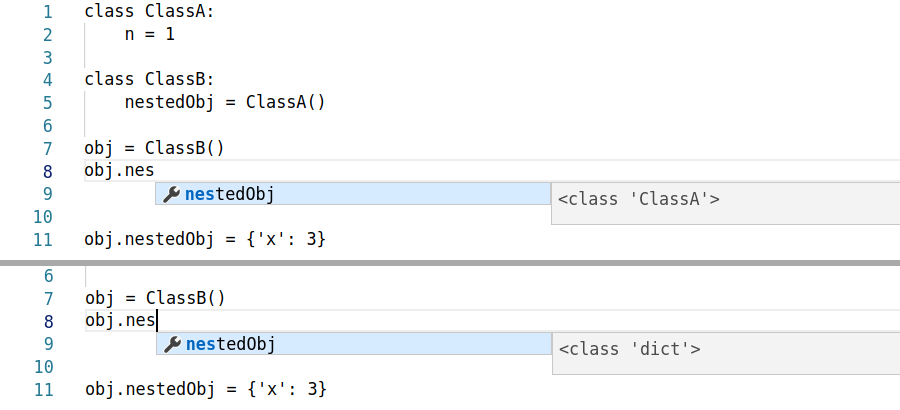
\includegraphics[width=\linewidth]{images/xp_report/limitation_cached_completion_Python.png}
%DIF <      \caption[Limitations of code completion using cached run-time information]{Code completion of properties without and with cached run-time information in GraalPython. In the upper part of the image, the completion is shown as expected, because the completion items were obtained from the run-time state at line 8 by executing the source code up to that line. In the lower part, run-time information have been collected for the whole source code and the completion items were obtained from the frame snapshot captured in line 7, whose stored \inlinecode{obj} instance is no deep copy and therefore includes the modification in line 11.}
%DIF <      \label{fig:xp:limitationCachedCompletionPython}
%DIF <  \end{figure}
%DIFDELCMD < 

%DIFDELCMD < %%%
%DIF <  Another problem of caching frame snapshots is that we hold references to arbitrary run-time objects which can therefore not be garbage collected. Depending on the size of the objects, the Java process might run out of memory, although this has not yet happened in our experiments.
%DIFDELCMD < 

%DIFDELCMD < %%%
%DIF <  Using cached frames for in-line evaluation, to improve the performance of \ac{lsp} responses, has another limitation. The executed source code must rely on data of the stored frame snapshot only. There is for example no call stack available and the language context storing the global run-time state might be different than it was at the moment when the snapshot was taken.
%DIFDELCMD < 

%DIFDELCMD < %%%
%DIF <  As already mentioned, we also reuse language contexts to avoid their expensive creation each time source code has to be executed. Unfortunately, this leads to similar global state problems as described for stored frame snapshots. For example in GraalPython, a module import is done only once per context. If the module's source code is changed and we reuse a context which has already imported that module, the changes will be ignored in further executing runs. Furthermore, after renaming functions, the old ones will still be suggested via code completion.
%DIFDELCMD < 

%DIFDELCMD < %%%
%DIF <  With regard to the numerous limitations which arise due to our current implementation of caching run-time information, we have to admit, that this part needs further improvements. It works well for context independent scripts, but is not yet mature enough for lager software projects.
%DIFDELCMD < 

%DIFDELCMD < %%%
%DIF <  \subparagraph{A Polyglot Language Server}
%DIF <  The Truffle framework allows hosting language implementations in a multi-language run-time environment. We have already explained, that \graallsp~supports polyglot code completion, but with some limitations. A language server is typically developed for exactly one language. During initialization, we have to tell the language client the set of completion and signature help trigger characters to support auto-activation. If the installed languages have different trigger characters, like a dot for GraalPython, a \inlinecode{\$} for FastR, and a space for GraalSqueak, a completion might be triggered in unwanted situations and might cancel other requests. FastR for example allows to use dots in variable identifiers, as can be seen in the already mentioned \autoref{fig:xp:completionGlobalsR}. Typing a dot in FastR code while having GraalPython installed, will trigger a code completion request. At server-side, we can detect, that the dot is no trigger character of FastR and return no completion items, but the current request, which might be a previous completion request of FastR, will be cancelled. Furthermore, Visual Studio Code displays a default, token-based code completion, if \graallsp~returns no results. This is quite confusing for the language users, because a language's code completion behavior might change depending on the set of installed languages.
%DIFDELCMD < 

%DIFDELCMD < %%%
%DIF <  Another limitation occurs for the code completion of properties of foreign objects, if the foreign languages have different syntaxes, as already described for FastR and GraalPython. The suggested properties are formatted in the syntax of the foreign language and might therefore yield a syntax or run-time error in the current language. It lies therefore in the responsibility of the developer to deal with mismatching syntaxes and transform suggested code elements, which do not match the language's syntax, to a generic, foreign message send using the polyglot \ac{api} of their current language.
%DIFDELCMD < 

%DIFDELCMD < %%%
\DIFdelend \section{Related Work}
\label{cha:relatedwork}

%DIF < As tooling support for programming languages is a wide field of research, we only focus on work related to language implementation frameworks for dynamic languages and language-agnostic tooling approaches for \acp{ide}.
\DIFdelbegin %DIFDELCMD < 

%DIFDELCMD < %%%
\DIFdelend Our approach focuses on enabling performance-focused language implementation
frameworks to provide their implemented dynamic languages with IDE-like tooling
support with minimal effort. Another major part of our approach is based on
collecting and using run-time information to enhance certain \ac{lsp} features.

%DIF <  To understand the challenging task of developing new languages and corresponding tools, we have to have a look at how existing and widely used \acp{ide} provide support for new languages. Among other \acs{ide}, Eclipse \cite{des2004eclipse}, VisualStudio \cite{Microsoft2018}, and IntelliJ \cite{JetBrains2018} provide extension points to develop \ac{ide}-specific plugins for new languages. Depending on the \ac{ide}, you have to implement lexer and parser yourself or provide at least grammar files to generate these components. Then, you have to manually implement further \ac{ide}-specific interfaces to support features like code completion, finding all references, or goto-definition. As already mentioned in \todo{motivation}, this will be difficult especially for dynamic languages. Another barrier for language or tool developers might be, that you have to implement these components in the \ac{ide}'s host language. Furthermore, if you want to support another \ac{ide}, the whole process needs to be repeated. The \ac{lsp} solves  some of these problems and the mentioned \acp{ide} support this protocol already. However, you still have to develope a language server for your language from scratch.
\DIFdelbegin %DIFDELCMD < 

%DIFDELCMD < %%%
\DIFdelend \ac{ide}-frameworks like Eclipse \cite{des2004eclipse}, Visual
Studio\footnote{\url{https://visualstudio.microsoft.com} (accessed 2018-12-17)},
or IntelliJ\footnote{\url{https://www.jetbrains.com/idea} (accessed 2018-12-17)}
provide extension points to develop \ac{ide}-specific plugins for new languages
or can be used as language clients if they implement the \ac{lsp}. But as they
do not support language developers in implementing programming languages in the
first place and writing \ac{ide}-specific plugins or a language server still
requires a lot of work, we do not further discuss them here. Furthermore, there
are lots of language- and editor-specific tooling solutions for dynamic
languages, which are also not our focus.

%DIF <  \clearpage
\DIFdelbegin %DIFDELCMD < 

%DIFDELCMD < %%%
%DIF <  \paragraph{Outline}
%DIF <  \begin{itemize}
%DIF <      % \item ??? Typical IDE-frameworks used by performance-focused language implementations
%DIF <      % \begin{itemize}
%DIF <      %     % Eclipse and IntelliJ -> you need to implement the custom IDE lang-specific parts in Java - you cannot use the language you implemented your language with
%DIF <      %     % You need to implement lexer and parser again and all other required interfaces - gap between impls
%DIF <      %     % These IDEs say, that you "only" have to implement the lang specific parts "with a small amount of effort"
%DIF <      %     % Features like code completion of properties and goto-definition are still hard to implement for dynamic languages
%DIF <      %     \item Eclipse
%DIF <      %     \item Visual Studio % https://docs.microsoft.com/en-us/azure/devops/integrate/ide/extensions/develop_extensions/add_new_language?view=vsts
%DIF <      %     \item IntelliJ 
%DIF <      %     % http://www.jetbrains.org/intellij/sdk/docs/reference_guide/custom_language_support.html
%DIF <      %     % http://www.jetbrains.org/intellij/sdk/docs/reference_guide/custom_language_support/code_completion.html
%DIF <      % \end{itemize}
%DIF <      \item Tools-first language implementation frameworks
%DIF <      \begin{itemize}
%DIF <          \item Language workbenches
%DIF <          \begin{itemize}
%DIF <              \item Xtext
%DIF <              % language development framework -> DSLs
%DIF <              % Xtext is a framework for development of programming languages and domain-specific languages. With Xtext you define your language using a powerful grammar language. As a result you get a full infrastructure, including parser, linker, typechecker, compiler as well as editing support for Eclipse, any editor that supports the Language Server Protocol and your favorite web browser
%DIF <              \item Spoofax and DynSem - generates a Truffle AST interpreter
%DIF <          \end{itemize}
%DIF <          \item Helvetia and Squimera
%DIF <      \end{itemize}
%DIF <      \item Language-agnostic Approaches Enabling \ac{ide}-like Features
%DIF <      \begin{itemize}
%DIF <          \item CTags
%DIF <          \item Kythe
%DIF <          \item srclib %https://srclib.org/
%DIF <          \item Lucid Energize 
%DIF <      \end{itemize}
%DIF <      \item Language-specific \ac{ide}-independent Feature Support
%DIF <      \begin{itemize}
%DIF <          \item Jedi (Python)
%DIF <          \item Rsense (ruby)
%DIF <          \item Tern (JS)
%DIF <      \end{itemize}
%DIF <      \item Improving \acs{ide} Features With Run-time Information
%DIF <      \begin{itemize}
%DIF <          \item Type harvesting
%DIF <          \item PyCharm - dynamic type inference for code completion
%DIF <          \item pyannotate - Insert annotations into your source code based on call arguments and return types observed at run-time
%DIF <          \item Hermion
%DIF <          \item Enhancing static ref search with dynamic data
%DIF <      \end{itemize}
%DIF <  \end{itemize}
%DIFDELCMD < 

%DIFDELCMD < %%%
%DIF <  \clearpage
%DIFDELCMD < 

%DIFDELCMD < %%%
%DIF <  \subsection{Tools-first Language Implementation Frameworks}
%DIFDELCMD < 

%DIFDELCMD < %%%
\DIFdelend Language Workbenches such as like Spoofax \cite{kats2010spoofax}, Xtext
\cite{eysholdt2010xtext}, or MPS \cite{voelter2012language} focus foremost on
the efficient definition, reuse and composition of languages and their
\acp{ide} \cite{erdweg2013state}. In contrast to the work presented here,
performance and generality of the resulting languages is a secondary concern.
%DIF <  \subparagraph{Language Workbenches} Language workbenches are tools that support
%DIF <  the efficient definition, reuse and composition of languages, especially
%DIF <  \acp{dsl} \cite{Fowler2010DomainSpecificLanguages}, and their \acp{ide}
%DIF <  \cite{erdweg2013state}. Hence, they provide the means to make the development
%DIF <  and composition of new languages affordable, which has been proven by the usage
%DIF <  of language workbenches and \acp{dsl} in various use cases in industry. Most
%DIF <  language workbenches support a textual language notation, which can be edited in
%DIF <  a free-form text editor. But there are also solutions like MPS
%DIF <  \cite{voelter2012language}, which allow projectional editing or mathematical
%DIF <  symbols. Furthermore, syntactic services (syntax highlighting, folding, or
%DIF <  syntactic completion), semantic services (reference resolution, refactoring,
%DIF <  diagnostics, or semantic completion), and further \ac{ide}-like features can be
%DIF <  provided based on the language definitions.
\DIFdelbegin %DIFDELCMD < 

%DIFDELCMD < %%%
%DIF <  However, as already described in \autoref{cha:introduction}, these frameworks do
%DIF <  not focus on the performance of the language implementations in the first place
%DIF <  and are often bound to a limited set of \acp{ide}. Furthermore, dynamic
%DIF <  languages cannot make use of all the services of language workbenches, as these
%DIF <  services typically rely on the static information derived from the language
%DIF <  definitions.
%DIFDELCMD < 

%DIFDELCMD < %%%
%DIF <  Xtext \cite{eysholdt2010xtext} is one of the first language workbenches, which
%DIF <  supports the \ac{lsp}, and which also proposes, that it can be used to develope
%DIF <  \acp{dsl} and full-featured programming languages. However, Xtext faces the same
%DIF <  challenges like the other workbenches, when it comes to dynamic languages, which
%DIF <  we try to tackle explicitly in \graallsp.
\DIFdelend 

Visser et al. described an approach using the Spoofax language workbench
\cite{kats2010spoofax} and the DynSem language
\cite{vergu_et_al:LIPIcs:2015:5208} to systematically generate Truffle
languages, i.e. \ac{ast} interpreters, from DynSem specifications
\cite{visser2014language}. However, Spoofax provides plugins for the Eclipse
\ac{ide} only. It would be interesting to see if \ac{lsp} support can easily be
enabled for Truffle \DIFdelbegin \DIFdel{language }\DIFdelend \DIFaddbegin \DIFadd{languages }\DIFaddend generated in this way.
    %DIF <  Supporting the \ac{lsp} seems to be planned, but is not yet
%DIF <  present. Hence, it would be worth to evaluate, if a Truffle language generated
%DIF <  through this approach could provide enough means to support at least some
%DIF <  \graallsp~features. Nonetheless, the generated interpreters will still require
%DIF <  manual tweaks, to benefit from all the GraalVM optimizations.

%DIF <  Language workbenches, a term popularized by Martin Fowler in 2005 [19], are tools that support the efficient definition, reuse and composition of languages and their IDEs. Language workbenches make the development of new languages affordable and, therefore, support a new quality of language engineering, where sets of syntactically and semantically integrated languages can be built with comparably little effort. This can lead to multi-paradigm and language-oriented programming environments [8, 61] that can address important software engineering challenges. \paragraph{Frameworks for DSLs}
    %DIF <  \begin{itemize}
    %DIF <      \item not performance focused
    %DIF <      \item typically only one or a very limited set of target IDEs supported (e.g. an Eclipse plugin)
    %DIF <      \item not limited to textual notation (also graphical, tabular etc.)
    %DIF <      \item Composability
    %DIF <      \item Testing / debugging
    %DIF <      \item Editing mode: free form + projectional
    %DIF <      \item Syntactic services (Highlighting, Outline, Folding, Syntactic completion, Diff, Auto formatting)
    %DIF <      \item Semantic services (Reference resolution, Semantic completion, Refactoring, Error marking, Quick fixes, Origin tracking, Live Translation)
    %DIF <  \end{itemize}
        \DIFdelbegin %DIFDELCMD < 

%DIFDELCMD <     %%%
%DIF < - stefan marr:  While Language Workbenches provide such features, I personally prefer the bottom up approach. Instead of specifying my language, I’d rather express the one truth of its semantics as an interpreter. In the end, I want to execute programs. So, let’s start there.
%DIFDELCMD < 

%DIFDELCMD <     %%%
%DIF <  \paragraph{Xtext}
    %DIF <  Xtext, part of the Eclipse project, is a framework for defining external DSLs in close cooperation with the Eclipse IDE. \cite{humer2015domain}
%DIFDELCMD < 

%DIFDELCMD <     %%%
%DIF <  \paragraph{A Language Designer's Workbench} \cite{visser2014language} use Spoofax and DynSem \cite{vergu_et_al:LIPIcs:2015:5208}
    %DIF <      % To support the direct execution of programs in the object language, we systematically generate a Java-based AST interpreter from a DynSem specification for the language. Each constructor of the language is translated to a class in Java with an evaluate method based on the DynSem rules for the constructor.
    %DIF <      % DynSem specifications are executable through automatic generation of a Java-based AST interpreter.
    %DIF <      -> generated AST-interpreter for Truffle <- can one modify the generated interpreter?
    %DIF <      -> end-user IDE: bound to the Spoofax generated editor(-plugin)
%DIFDELCMD < 

%DIFDELCMD <     %%%
%DIF <  \paragraph{Ensō} http://enso-lang.org
    %DIF <      -> Ensō is a self-describing workbench based entirely on interpreters implemented in an object-oriented language. Ensō avoids the generation of code and follows the hypothesizes, that interpreters are easier to develop and combine than compilers or transformational approaches. Because Ensō is implemented in itself, all available tools in the system can be reused to create applications. -> Smalltalk approach
    %DIF <      % Ensō rejects the common approaches for 1) model to code, 2) model to model, and 3) generic transformation languages.
    %DIF <      % Ensō is based entirely on interpreters not compilers/translators. Code generation is completely avoided, because it is complex and unnecessary. Ensō hypothesizes that interpreters are easier to develop, maintain, extend, and combine than compilers/transformations. As examples, both the Ensō data modeling language [1] and grammar language [2] are interpreted on the fly.
    %DIF <      % Ensō implements interpreters using ordinary object-oriented code. By defining interpreters as objects, traditional object-oriented composition and inheritance techniques can be used to extend and combine language semantics.
    %DIF <      % Ensō is based on external languages rather than embedding. An external language is one that has its own syntax and semantics, independent of any other language. An embedded language is defined as a library within a host language. Embedded languages typically reuse features of the host language, including variable binding or control flow.
    %DIF <      % Ensō strikes out on its own rather than building on existing standards, including UML and EMF.
    %DIF <      % Eclipse is a powerful and practical platform with many advantages. However, it is possible that much of its complexity is accidental rather than fundamental. If so, it may be possible to create an extensible integrated development environment with orders of magnitude less code and complexity than in Eclipse. To find out, Ensō will create its own IDE rather than build on top of Eclipse. Evidence from Newspeak, Cloud9, and Smalltalk suggest that this is possible.
    %DIF <      % Finally, Ensō is implemented in itself. This allows all tools written for the system to be reused in creating applications, and tools and libraries developed for applications to be reused in the creation of the system. It also means that the core languages and strategies that define the Ensō system can be modified to extend the functionality of Ensō. Smalltalk has shown the benefits of such deep reflection. Ensō provides a similar level of reflection, but in a more controlled way, as the system has a well-defined bootstrap process. Ensō is bootstrapped from Ruby, and is available today for experimentation.
    %DIF <      % [1] Alex Loh, Tijs van der Storm, William R. Cook. “Managed Data: Modular Strategies for Data Abstraction” To appear SPLASH Onward! 2012. http://www.cs.utexas.edu/~wcook/Drafts/2012/ensodata.pdf
    %DIF <      % [2] Tijs van der Storm, Alex Loh and William R. Cook. “Object Grammars: Compositional & Bidirectional Mapping Between Text and Graphs” To appear at the International Conference on Software Language Engineering (SLE), 2012. http://www.cs.utexas.edu/~wcook/Drafts/2012/ensogrammars.pdf
    %DIF <      % https://modeling-languages.com/enso-dont-design-your-programs-program-your-designs/
    %DIFDELCMD < 

%DIFDELCMD < %%%
%DIF <  \subparagraph{Helvetia and Squimera}
\DIFdel{Two approaches , which }\DIFdelend \DIFaddbegin \DIFadd{Two approaches that }\DIFaddend focus on reusing existing tools of a live programming
environment and the overall programming experience, are the Smalltalk-based
\acp{ide} Helvetia \cite{renggli2010embedding} and Squimera
\cite{niephaus2018live}. Helvetia enables embedding \acp{dsl} into Smalltalk, by
adding hooks into the Smalltalk compiler chain. This way, the \acp{dsl} can be
translated on demand into Smalltalk code, so that existing tools of the
environment still work, without the need to generate and start a new
\ac{ide}. Squimera composes RPython interpreters into an RPython-based Smalltalk
\ac{vm} to re-use the Smalltalk tools for all composed languages. In contrast to
this work, these approaches focus on Squeak/Smalltalk as the \ac{de}.

%DIF <  Squimera is not a language implementation framework, but it enables polyglot programming and debugging through the composition of interpreters written in RPython. With some adjustments, some of the existing Smalltalk tools have been made reusable for writing and debugging Python and Ruby code, providing a consistent programming experience across languages. Like \graallsp, Squimera utilizes the interpreters and \acp{api} of a performance-focused language implementation framework, to retrieve data needed for the tools of the language users.
    %DIF < Like in Helvetia, no new \ac{ide} instance needs to be started to use other languages, as the environment is part of the Smalltalk language and runs in the same process.
\DIFdelbegin %DIFDELCMD < 

%DIFDELCMD <     %%%
%DIF <  Helvetia and Squimera provide syntax highlighting and debugging support for the integrated languages, but features like code completion or goto-definition are only provided at Smalltalk level. However, the integrated languages could theoretically make use of all the tools of the Smalltalk environment. In Squimera, customized tools for polyglot programming of high-level languages have been created and are still a subject of research. This would not be possible in \acp{ide} using \graallsp~yet, as they are bound on the one hand to the features made available through the Truffle instrumentation \ac{api} and on the other hand to the specification of the \ac{lsp}.
    %DIFDELCMD < 

%DIFDELCMD <     %%%
%DIF <  \subparagraph{}
    %DIF <  In summary, language workbenches and the other described approaches can provide a richer, more customized, and domain-specific tooling support for new or existing languages than \graallsp. However, these solutions are not able to create high-performance dynamic languages together with tools for the users of the languages, supporting \ac{ide} features like code completion or goto-definition. Furthermore, the users are often bound to a single \ac{ide}, whereas \graallsp~allows them to choose from a variety of \ac{lsp} clients.
%DIFDELCMD < 

%DIFDELCMD < %%%
%DIF <  \subsection{Language-agnostic Approaches Enabling \ac{ide}-like Features}
%DIFDELCMD < 

%DIFDELCMD < %%%
%DIF <  To the best of our knowledge, there are no approaches comparable to the
%DIF <  \acl{lsp} yet, which are supported by almost all popular source code editors and
%DIF <  languages. However, there exist other approaches for language-agnostic tooling
%DIF <  support, which can be seen as predecessors or influencer for \ac{lsp}. These
%DIF <  include tools like Ctags that create language-agnostic index files for symbols
%DIF <  in source code for consumption by various code editors.
%DIFDELCMD < 

%DIFDELCMD < %%%
%DIF <      \subparagraph{Ctags}
%DIF <      % \begin{itemize}
%DIF <      %     % The ctags and etags programs (hereinafter collectively referred to as ctags, except where distinguished) generate an index (or "tag") file for a variety of language objects found in file(s). This tag file allows these items to be quickly and easily located by a text editor or other utility. A "tag" signifies a language object for which an index entry is available (or, alternatively, the index entry created for that object). Alternatively, ctags can generate a cross reference file which lists, in human readable form, information about the various source objects found in a set of language files. Tag index files are supported by numerous editors, which allow the user to locate the object associated with a name appearing in a source file and jump to the file and line which defines the name.
%DIF <      %     % Exuberant CTAGS http://ctags.sourceforge.net/
%DIF <      %     %\item \cite{hiebert1999exuberant} % Exuberant CTAGS http://ctags.sourceforge.net/
%DIF <      %     \item \footnote{\url{http://ctags.sourceforge.net} (accessed 2018-12-17)}
%DIF <      %     \item tagging a language object in an index file
%DIF <      %     \item tag-file supported by editors
%DIF <      %     \item allows user to locate the tagged object via name (goto-definition, list symbols)
%DIF <      %     \item for new languages you need to define a regex or parser to find language objects
%DIF <      %     \item only static analysis, no scoped completion (everything is suggested)
%DIF <      % \end{itemize}
%DIF <      % Ctags is an old but still popular tool to create language-agnostic index (tag) files for symbols found in source code of various programming languages. The tags can be consumed by source code editors to provide a goto-definition search or a simple symbol completion. Over the years different flavors of the original Ctags have come up which extended the original file format for tags. A popular variant, Exuberant Ctags\footnote{\url{http://ctags.sourceforge.net} (accessed 2018-12-16)}, was originally distributed with Vim, but became a separate project, supporting over 40 programming languages. New languages can be added either by defining regular expressions to determine language symbols, or providing a parser.
%DIFDELCMD < 

%DIFDELCMD <     
%DIFDELCMD < %%%
%DIF <      \subparagraph{Energize} Energize/Cadillac \cite{gabriel1990foundation} was
%DIF <      an object-oriented \ac{ide} for C++ built upon Emacs in the late 1980s. It
%DIF <      was based on a language-agnostic client-server architecture for programming
%DIF <      language environments. Clients (compilers, editors, debuggers, etc.)
%DIF <      communicate with a server using protocols for a certain class of tools
%DIF <      (compiler protocol, editor protocol, debugger protocol, etc.). The server is
%DIF <      able to persistently store objects that represent source code, language
%DIF <      elements, compiled code objects, and annotations (objects which are links
%DIF <      between other objects), so that each tool can access the needed
%DIF <      information. For example, annotations could be used to link compiler
%DIF <      diagnostics to source code and/or language elements, but also to retain
%DIF <      dependencies to enable incremental compilation. The persistent object store
%DIF <      was intended to store information, such as dependency analyses, for the
%DIF <      lifetime of the software. New languages could be added, by providing
%DIF <      compilers for these languages, which support the compiler protocol.
    %DIFDELCMD < 

%DIFDELCMD < %%%
%DIF <      The \ac{lsp} could be interpreted as an evolved version of selected parts of
%DIF <      the Energize protocols, especially of editor and compiler.
   %DIFDELCMD < 

%DIFDELCMD < %%%
%DIF <      % In the late 1980s, we started working at Lucid on a programming environment for C/C++. It was based on a programming-language-neutral, non-abstract-syntax-tree way of describing programs, annotations (a generalization of hypertext), a persistent repository for program information, and a tool-neutral user-interaction mechanism. To this day I have not seen a programming environment as advanced as Energize/Cadillac (official name/code name). There was really only one substantial paper published about the work, and that was in an obscure conference called C++ At Work (sorry if this offends someone). The paper was called Foundation for a C++ Environment (http://www.dreamsongs.com/Cadillac.html)
%DIFDELCMD < 

%DIFDELCMD < %%%
%DIF <      \subparagraph{Kythe}
%DIF <      Kythe\footnote{\url{https://kythe.io} (accessed 2018-12-16)} is a pluggable, language-agnostic ecosystem for building tools that work with code. Kythe allows language analysis and indexing to be run as services, by defining language-agnostic protocols and data formats for representing, accessing, and querying source code information as data. It was originally developed as an internal Google project, due to the observation that most companies have projects which are created with more than three programming languages, but lack appropriate cross-language tools\footnote{\url{https://bsumm.net/2012/08/11/steve-yegge-and-grok.html} (accessed 2018-12-16)}. To support a new language in Kythe, a language compiler or interpreter needs to be extended, so that it can emit a rich \ac{ast}, symbol table, and type graph in a Kythe-compliant intermediate representation. For dynamic languages however, the generated \acp{ast} do not include the information required by Kythe, so that additional type inference engines are needed.
%DIFDELCMD < 

%DIFDELCMD < %%%
%DIF <      \subparagraph{srclib}
%DIF <      Another project which tried to tackle similar challenges as \ac{lsp} is srclib\footnote{\url{https://srclib.org} (accessed 2018-12-16)}, a polyglot code analysis library for static analysis and code search. srclib was the foundation of Sourcegraph\footnote{\url{https://sourcegraph.com} (accessed 2018-12-16)}, a code search and intelligence server that helps developers to find, review, and understand code. Like \ac{lsp}, srclib defined a language-agnostic format, which can be consumed by development tools. New languages can be supported by implementing a tool chain that outputs the srclib format. For languages like JavaScript, Ruby, and Python, tool chains have been built reusing existing language-specific projects like Tern, YARD\footnote{\url{https://yardoc.org} (accessed 2018-12-16)}, and Jedi. However, with the upcoming of \ac{lsp}, the development of srclib was stopped and Sourcegraph also makes use of \ac{lsp} now.
%DIF <      %-> not under active development anymore, Sourcegraph uses LSP now
%DIF <      % srclib makes developer tools like code search and static analyzers better. It supports things like jump to definition, find usages, type inference, and documentation generation.
%DIF <      % srclib consists of language analysis toolchains (currently for Go, Python, JavaScript, and Ruby) with a common output format, and developer tools that consume this format.
%DIF <      % srclib originated inside Sourcegraph, where it powers intelligent code search over hundreds of thousands of projects.
%DIF <      % srclib takes care of the code analysis that underlies key assistive features such as finding usages and jumping to definitions. It exposes a command-line API and outputs data in a well defined, language-independent format.
%DIF <      % A plugin (or other tool) built on srclib just has to consume this data format to support all languages that srclib supports. srclib is designed to be modular and extensible. New languages can be added by implementing language toolchains that output the srclib format.
%DIF <      % srclib is 100% open source and built on other well-established open-source projects like Tern, YARD, and Jedi.
%DIF <      % Sourcegraph https://sourcegraph.com is a free, open-source, self-hosted code search and intelligence server that helps developers find, review, understand, and debug code. Use it with any Git code host for teams of any size. Start using it now, then install the Sourcegraph Docker image on your private code.
%DIF <      % Solve problems before they exist, commit by commit. Code intelligence makes browsing code easier, with IDE-like hovers, go-to-definition, and find-references on your code, powered by Sourcegraph extensions and language servers based on the open-source Language Server Protocol
%DIFDELCMD < 

%DIFDELCMD < %%%
%DIF <      \subparagraph{}
%DIF <      Like the \ac{lsp}, the described tools and approaches define more or less complex protocols to decouple languages and their development tools. Supporting a new language ranges from adding only a regular expression to implementing or instrumenting complex compilers, to output language-specific information in a language-agnostic format. However, code completion is not part of these protocols, which we wanted to support in \graallsp. Furthermore, besides \ac{lsp}, only Ctags is supported by a variety of source code editors and \acp{ide} at the date of writing.
%DIFDELCMD < 

%DIFDELCMD < %%%
%DIF <  \subsection{Language-specific Editor-agnostic Approaches Enabling \ac{ide}-like Features}
%DIF <      As described in the introductory words to this chapter, there are lots of \ac{ide}- or editor-specific solutions to support code completion etc. for certain dynamic languages, which are not discussed here. But there are some language-specific solutions worth mentioning, which are designed to be editor-independent, like Jedi\footnote{\url{https://github.com/davidhalter/jedi} (accessed 2018-12-19)} for Python, Tern\footnote{\url{http://ternjs.net} (accessed 2018-12-19)} for JavaScript, or Rsense\footnote{\url{https://github.com/rsense/rsense} (accessed 2018-12-19)} for Ruby. Like \ac{lsp}, Tern and Rsense define a lightweight interchange format, so that editor-plugins can be created, which only have to map the requests and responses to their editor-specific \ac{api}. Tern and Rsense provide a server which accepts and responds \ac{json} messages. However, the structure of the messages is influenced by the corresponding language and is therefore more specific than the message format of \ac{lsp}. Jedi provides a simple Python \ac{api} only. Therefore, editor-plugins need to be able to execute Python code or support the \ac{lsp}, because there already exist Python language servers using Jedi.
%DIFDELCMD < 

%DIFDELCMD < %%%
%DIF <      All the described tools mainly rely on static code analysis, so that they all face limitations due to certain dynamic features of their corresponding language. Jedi was originally intended to provide a rich code completion by executing non-dangerous code, which did not work, so that a highly recursive static analyzer has been created\footnote{\url{https://jedi.readthedocs.io/en/latest/docs/features.html\#a-little-history}\\(accessed 2018-12-19)}. \graallsp~is able to execute source code to some extent yet, so that it supports code completion also for dynamic features. However, as the described solutions are language-specific, they can support certain features more suitable and with more detail than a generic \ac{lsp}. But this comes at another cost, because these tools cannot reuse the existing language parsers to get the required data. They had to built and maintain separate parsers, so that when the languages evolve, there might always be a gap between language elements already supported in the original parsers, which have not been implemented in the parsers of the tools yet. In contrast, \graallsp~can indirectly utilize the existing language parsers through the Truffle \ac{api}.
%DIFDELCMD < 

%DIFDELCMD < %%%
%DIF <  \subsection{Improving \acs{ide} Features With Run-time Information}
%DIF <  \label{sec:rw:collectionRunTimeInformation}
    %DIF <  \begin{itemize}
    %DIF <      \item Type harvesting \cite{haupt2011type}
    %DIF <      \item Hermion \cite{rothlisberger2008exploiting}
    %DIF <      %\item Nemo Bachelor Project? -> sandboxed execution in Squeak
    %DIF <      \item https://github.com/dropbox/pyannotate ->  Insert annotations into your source code based on call arguments and return types observed at runtime. - uses Python's sys.setprofile(profilefunc)
    %DIF <      \item https://blog.jetbrains.com/pycharm/2013/02/dynamic-runtime-type-inference-in-pycharm-2-7/
    %DIF <      \item Enhancing Static Source Code Search With Dynamic Data \cite{holmes2010enhancing}
    %DIF <  \end{itemize}
%DIFDELCMD < 

%DIFDELCMD < %%%
\DIFdel{A major part }\DIFdelend \DIFaddbegin \DIFadd{Part }\DIFaddend of our approach focuses on collecting and utilizing run-time information to
answer \ac{lsp} requests. %DIF <  Therefore, we have a look at where and how other approaches apply run-time information to improve \ac{ide} features.
There are a number of \DIFdelbegin \DIFdel{interesting prior approaches to }\DIFdelend \DIFaddbegin \DIFadd{prior approaches towards }\DIFaddend this
idea.

%DIF <  \subparagraph{Hermion}
    %DIF <  % We address these questions and present our working prototype, an IDE called Hermion with the capability to capture runtime information from an application under development and to exploit this information by enhancing navigation and browsing of the source code.
The Hermion \ac{ide} \cite{rothlisberger2008exploiting} collects run-time
information to enhance program comprehension by improving static source code
navigation and browsing in Squeak/Smalltalk. %DIF <  In detail, they apply a filter to
%DIF <  the list of methods of the implementers view to display only those methods which
%DIF <  have been called in a specific scenario. Furthermore, they display collected
%DIF <  type information for instance variables and provide an additional reference view
%DIF <  in the method source code view, that shows a list of observed classes which are
%DIF <  referenced in the current method.
Hermion builds upon partial
behavioral reflection \cite{tanter2003partial} to restrict the collection of
run-time information to certain source code parts and detail levels. However,
\DIFdelbegin \DIFdel{due to performance issues, the users of the Hermion
\mbox{%DIFAUXCMD
\ac{ide} }\hspace{0pt}%DIFAUXCMD
have to make a trade-off between performance and the amount of
collected information. The }\DIFdelend users need to manually specify which classes shall be instrumented \DIFdelbegin \DIFdel{, }\DIFdelend to keep the
cost of instrumentation and reflective operations at an acceptable level. In
\graallsp, the set of \DIFdelbegin \DIFdel{\mbox{%DIFAUXCMD
\ac{ast} }\hspace{0pt}%DIFAUXCMD
nodes which shall be
instrumented when collecting and caching run-time information, }\DIFdelend \DIFaddbegin \DIFadd{instrumented \mbox{%DIFAUXCMD
\ac{ast} }\hspace{0pt}%DIFAUXCMD
nodes }\DIFaddend is implicitly defined by the
\ac{lsp} workspace, i.e. all parsed source code files. As \DIFdelbegin \DIFdel{we
collect snapshots of frames, we increase performance and reduce the amount of
collected instances by taking only the first frame which is reported for every
instrumented node. As }\DIFdelend Hermion continuously
observes the instrumented classes, it can collect different types for a
variable, which the current \graallsp~implementation \DIFdelbegin \DIFdel{would not be able to detect}\DIFdelend \DIFaddbegin \DIFadd{does not do}\DIFaddend .

%DIF <  \begin{itemize}
    %DIF <      \item Hermion builds upon partial behavioral reflection \cite{tanter2003partial} to restrict the collection of run-time information only to certain source code parts and detail levels. This is similar to Truffle's instrumentation of relevant \ac{ast} nodes, which we use in \graallsp. % E. Tanter, J. Noye, D. Caromel, and P. Cointe. Partial Behavioral Reflection: Spatial and Temporal Selection of Reification. In Proc. of the Conference on Object-oriented Programing, Systems, Languages, and Applications, pages 27–46. ACM, October 2003
    %DIF <      % Another approach to gain performance is partial behavioral reflection [Tanter et al. 2003], which restricts the application of a MOP in spatial and temporal manner. Instead of applying to all program parts equally, the developer optimizes the MOP’s application to only the places where it is needed to avoid unnecessary overhead. However, this does not reduce the cost of reflective operations used. Furthermore, it burdens again the programmer with the optimization while dispatch chains are part of the language implementation and thus optimize reflective operations without programmer intervention
    %DIF <      \item developer needs to manually specify which classes shall be instrumented
    %DIF <      \item due to performance issues, developers have to make a trade-off between performance and collected information
    %DIF <      \item similar to us: they rely on coverage of executed code
    %DIF <  \end{itemize}
\DIFdelbegin %DIFDELCMD < 

%DIFDELCMD <     %%%
%DIF <  \subparagraph{Enhancing Static Source Code Search in Eclipse}
\DIFdelend Holmes and Notkin \cite{holmes2010enhancing} described an approach to improve
the static find-references feature of the Eclipse \ac{ide} using collected
run-time information. Only executed methods are included in the search results,
so that users benefit from a limited result set related to their current
application. To collect the required run-time information, they \DIFdelbegin \DIFdel{use a custom
AspectJ \mbox{%DIFAUXCMD
\cite{kiczales2001overview} }\hspace{0pt}%DIFAUXCMD
aspect for }\DIFdelend \DIFaddbegin \DIFadd{instrument }\DIFaddend the
application's \DIFdelbegin \DIFdel{test
harness. %DIF <  Holmes and Notkin [15] describe an approach when the “find references” capability of an IDE is filtered using information from dynamic analysis – only methods executed in the given scenario are returned.
Our }%DIFDELCMD < \graallsp%%%
\DIFdel{~prototype does not utilize }\DIFdelend \DIFaddbegin \DIFadd{tests with AspectJ \mbox{%DIFAUXCMD
\cite{kiczales2001overview}}\hspace{0pt}%DIFAUXCMD
. This is comparable
to the case when }\DIFaddend run-time \DIFdelbegin \DIFdel{information to answer the }\emph{\DIFdel{references}} %DIFAUXCMD
\DIFdel{request of the \mbox{%DIFAUXCMD
\ac{lsp} }\hspace{0pt}%DIFAUXCMD
yet. We perform a static symbol-based
search in files of the current workspace, but it should be possible to enhance
our implementation of the }\emph{\DIFdel{references}} %DIFAUXCMD
\DIFdel{request in a similar way}\DIFdelend \DIFaddbegin \DIFadd{data is available in our approach}\DIFaddend .

%DIF <  \subparagraph{PyCharm Debugger}
\DIFdelbegin %DIFDELCMD < 

%DIFDELCMD < %%%
\DIFdelend \emph{Type harvesting} is another approach to collect type information for
dynamic programming languages~\cite{haupt2011type}. The solution is based on
\DIFdelbegin \DIFdel{a
stepwise execution of bytecode while }\DIFdelend observing the types of \DIFdelbegin \DIFdel{relevant
components}\DIFdelend \DIFaddbegin \DIFadd{variables during test execution}\DIFaddend . A similar feature exists
in the PyCharm \ac{ide} which can collect \DIFdelbegin \DIFdel{runtime }\DIFdelend \DIFaddbegin \DIFadd{run-time }\DIFaddend information during a debug
session. \DIFdelbegin \DIFdel{Inspired by these approaches we also
imagine unit tests as entry points for such type collection. }\DIFdelend \graallsp~has the advantage of running \DIFdelbegin \DIFdel{the collection }\DIFdelend with the \ac{jit} \DIFaddbegin \DIFadd{even when
instrumented}\DIFaddend , yielding better performance than these approaches.

%DIF <  In contrast to our approach, \emph{type harvesting} continuously
%DIF <  observes the stepwise execution of bytecodes in a live programming
%DIF <  system. However, the simulated stepwise execution is quite slow.  \graallsp, on
%DIF <  the other hand, benefits from Truffle's instrumentation and optimizations of
%DIF <  \ac{ast} nodes, so that the execution of instrumented nodes has a very small
%DIF <  overhead.
\DIFdelbegin %DIFDELCMD < 

%DIFDELCMD < %%%
%DIF <  PyCharm is a feature-rich \ac{ide} for the Python programming language. The
%DIF <  debugger of PyCharm is able to optionally collect run-time type information
%DIF <  during a debug
%DIF <  session\footnote{\url{https://blog.jetbrains.com/pycharm/2013/02/dynamic-runtime-type-inference-in-pycharm-2-7}
%DIF <    (accessed 2018-12-16)}. This information are used to improve code completion
%DIF <  and documentation popups during and after the debugging session. % The collected
%DIF <  % type information can also be persisted as docstrings in Python source code.
%DIF <      % PyCharm’s debugger is now capable of collecting type information at runtime and using this information for improving code completion suggestions, code insight and quick documentation popups. This needs to be enabled in the debugger settings.
%DIF <      % You debug your code all the time, and now in the course of debugging you can also collect type information. Afterwards, it will be used in auto-completion, and you will be able to put the collected type information into docstrings as well. Please note that enabling this feature may affect debugger performance, so use it with care.
%DIF <  Similar to our approach, the PyCharm's debugger can utilize unit tests as entry
%DIF <  point.
%DIF <  %
%DIFDELCMD < 

%DIFDELCMD < %%%
%DIF <  However, \graallsp~does not require to run code in a special (and slow)
%DIF <  debug mode to collect run-time information and can also make use of these
%DIF <  information to provide a precise goto-definition for callables.
%DIF <  For the PyCharm
%DIF <  \ac{ide}, this kind of dynamic run-time type inference is a small addition to
%DIF <  the other mature features, which rely on static analysis, whereas for \graallsp,
%DIF <  most features rely on run-time information. 
%DIFDELCMD < 

%DIFDELCMD < %%%
%DIF <  Both Hermion \ac{ide} and PyCharm's debugger collect types and are able to
%DIF <  remember all variants of variables, whereas \graallsp~currently collects one
%DIF <  snapshot per location. This way, \graallsp~can provide code completion items
%DIF <  also for properties of an object which are per-object and not defined in the
%DIF <  type.
%DIFDELCMD < 

%DIFDELCMD <     %%%
%DIF <  \subparagraph{}
    %DIF <  \begin{itemize}
    %DIF <      \item all these solutions are language-specifically implemented
    %DIF <      \item focus on a single aspects (code navigation, information on hover, or code completion)
    %DIF <      \item they need to be triggered manually, we do auto-exec in sandbox
    %DIF <      \item we can do a specific run to the location we are interested and collect only a single run-time object
    %DIF <  \end{itemize}
    %DIF <  In summary, all the three described solutions collect language-specific run-time information to improve certain static aspects of existing language-specific tooling. Hermion focuses on code navigation and comprehension, the approach of Holmes and Notkin on finding all references, and PyCharm on code completion and documentation. In contrast, \graallsp~collects run-time information in a language-agnostic way and tries to support as much \ac{ide} features as possible with this information. \graallsp~uses static approaches rather as fallback when no run-time information can be retrieved.
%DIFDELCMD < 

%DIFDELCMD <     %%%
%DIF <  \subparagraph{}
    %DIF <  The following two approaches do not directly target to improve specific \ac{ide} features, but they describe how to collect run-time information, so that other tools can make use of them. 
%DIFDELCMD < 

%DIFDELCMD <     %%%
%DIF <  \subparagraph{PyAnnotate}
    %DIF <  PyAnnotate\footnote{\url{https://github.com/dropbox/pyannotate} (accessed 2018-12-16)} is a Python library to collect type information (call arguments and return types) at run-time, using a Python-specific profiling hook. After a collection run, this information can be automatically inserted as annotations or comments into the Python source code, so that other tools can make use of them.
%DIFDELCMD < 

%DIFDELCMD <     %%%
%DIF <  \graallsp~collects run-time objects to answer \ac{lsp} requests only. The objects or their types are not persisted in the source code files for the later use of other tools.
%DIFDELCMD < 

%DIFDELCMD <     %%%
%DIF <  \subparagraph{Type Harvesting}
%DIFDELCMD < 

%DIFDELCMD < %%%
\DIFdelend \section{Conclusion and Future Work}
\label{cha:conclusion}

\DIFdelbegin \DIFdel{In this work, we }\DIFdelend \DIFaddbegin \DIFadd{We }\DIFaddend described the problem of language implementation frameworks lacking \DIFdelbegin \DIFdel{\mbox{%DIFAUXCMD
\ac{ide}}\hspace{0pt}%DIFAUXCMD
-like }\DIFdelend tooling
support for \DIFaddbegin \DIFadd{code editing, especially for }\DIFaddend implementations of dynamic programming
languages. Language developers that use such frameworks to create and maintain
programming languages with reasonable effort and good performance currently get
at most some run-time tooling. We propose an approach to have \ac{ide}-like \DIFdelbegin \DIFdel{tooling from the run-time information available in those frameworks }\DIFdelend \DIFaddbegin \DIFadd{code
assistance }\DIFaddend with minimal work required from the language developers. Our approach
is based on a language-agnostic \ac{lsp} server and collection and utilization
of run-time information. As proof of concept, we have implemented \graallsp, a
language server for the GraalVM.

% It uses the instrumentation \ac{api} of the Truffle language implementation
% framework, to parse and execute source code of Truffle languages and answer
% \ac{lsp} requests. No separate parser or inference engine is required. A
% sandboxing of the file system avoids unwanted side-effects when executing
% arbitrary source code. As by-product of using the Truffle framework,
% \graallsp~supports a polyglot code completion and goto-definition. Furthermore,
% we have suggested small \ac{api} extensions for Truffle, to support more
% \ac{lsp} features. They have been implemented in selected Truffle languages,
% together with other yet unsupported parts of the Truffle \ac{api}. As a result,
% we could demonstrate, that a basic set of important \ac{lsp} features can be
% supported for most of these languages with minimal implementation effort.

\DIFdelbegin \DIFdel{Two }\DIFdelend \DIFaddbegin \DIFadd{There are three }\DIFaddend limitations of our approach \DIFdelbegin \DIFdel{are the use of language runtime parsers and the
sandboxing while gathering run-time information. Since the runtime parsers typically stop parsing }\DIFdelend \DIFaddbegin \DIFadd{to consider especially: First, since
most runtime parsers stop }\DIFaddend on the first syntax error, we cannot report more than
one syntax error per file to the client. \DIFdelbegin \DIFdel{Furthermore}\DIFdelend \DIFaddbegin \DIFadd{Second}\DIFaddend , all \ac{lsp} features rely on
the availability \DIFdelbegin \DIFdel{parsed \mbox{%DIFAUXCMD
\ac{ir} }\hspace{0pt}%DIFAUXCMD
to query, so the sourcecode always needs to be
parsable for things like completion to work. Regarding the latter issue}\DIFdelend \DIFaddbegin \DIFadd{parseable source. Third}\DIFaddend , when our sandboxing prevents some kind
of access or triggers a timeout, some source sections of interest may not be
covered and thus no or only incomplete information is available.

% \subparagraph{Reusing Existing Language Parsers} We proposed in our approach to
% reuse the existing language parsers of performance-focused language
% implementations. As these parsers typically stop parsing on the first syntax
% error, we cannot report more than one syntax error per file to the
% client. Furthermore, all \ac{lsp} features rely on the availability of \ac{ast}
% nodes, to query for static information or to execute them to collect run-time
% information. Therefore, the source code needs to be parsable. However, when
% writing source code, there are situations were programmers edit the code in
% different areas in parallel, so that there might be multiple parts containing
% syntax errors. Reverting only the last change would not help in these cases to
% get the source code into a parsable state, so that most \ac{lsp} features would
% not work.

% \subparagraph{Language Server Protocol} A noticeable shortcoming of the \ac{lsp}
% is the lack of being able to provide hints for syntax highlighting from
% server-side. Syntax highlighting helps to read and understand source code,
% especially if it is an unfamiliar language. Although most editors support the
% usage of editor-independent formats like TextMate grammar
% files\footnote{\url{https://macromates.com/manual/en/language_grammars}
%   (accessed 2018-12-20)}, it is an additional effort for the language developers
% to provide and maintain these files for multiple editors. However, a support for
% semantic coloring is planned for a future version of \ac{lsp}, which might be
% exploited also for syntax highlighting.

% As the \ac{lsp} is an abstraction over a set of typical \ac{ide} features and we
% add another layer of abstraction for GraalVM languages, there will most likely
% be language-specific \acp{ide}, which can provide a more tailor-made and
% suitable tooling support than we can provide with \graallsp.

% \subparagraph{Reusing Existing Language Parsers} We proposed in our approach to
% reuse the existing language parsers of performance-focused language
% implementations. As these parsers typically stop parsing on the first syntax
% error, we cannot report more than one syntax error per file to the
% client. Furthermore, all \ac{lsp} features rely on the availability of \ac{ast}
% nodes, to query for static information or to execute them to collect run-time
% information. Therefore, the source code needs to be parsable. However, when
% writing source code, there are situations were programmers edit the code in
% different areas in parallel, so that there might be multiple parts containing
% syntax errors. Reverting only the last change would not help in these cases to
% get the source code into a parsable state, so that most \ac{lsp} features would
% not work.

% \subparagraph{Executing Source Code} Numerous features of our approach rely on
% run-time information, which we collect by executing source code. However, this
% implies, that our approach does not work well if we cannot provide these
% information. For example, if the sandboxing prevents some kind of I/O access,
% the source section of interest is not covered by the current execution, or a
% timeout triggers an exception. Therefore, the quality of our approach and the
% overall user experience might vary greatly depending on the source code and the
% available run-time information.

Future work is two-fold: the main work will be to address the above limitations
and find ways around them for realistic scenarios. \DIFaddbegin \DIFadd{This includes measuring how
much time we can afford to spent executing code before the user gives up waiting
for a result. }\DIFaddend The other is to cover more \ac{lsp} features in our approach. Part
of this means to investigate further how languages such as Squeak, which use
bytecodes as part of the execution model and do not map to files, can be made to
work with \ac{lsp}.
\DIFdelbegin \DIFdel{We also think making our
language server work better with polyglot programs must be part of this.
}\DIFdelend 

Despite these limitations, we already feel that our approach leads to a quickly
usable \DIFdelbegin \DIFdel{development environment from a language userpoint of view. On the other hand, it minimizes the burden on the side of language implementers
as \mbox{%DIFAUXCMD
\ac{lsp} }\hspace{0pt}%DIFAUXCMD
now comes almost for free with Truffle.
Furthermore, }\DIFdelend \DIFaddbegin \DIFadd{code editor for the language user. Since we use the instrumentation }\api
\DIFadd{of the Truffle framework to parse and execute source code and answer \mbox{%DIFAUXCMD
\ac{lsp}
}\hspace{0pt}%DIFAUXCMD
requests, no separate parser or inference engine is required. Sandboxing avoids
unwanted side-effects when executing arbitrary source code. As by-product of
using the Truffle framework, }\graallsp\DIFadd{~supports polyglot editing
assistance. With few }\api \DIFadd{extensions for Truffle languages to implement we
demonstrated that a basic set of important \mbox{%DIFAUXCMD
\ac{lsp} }\hspace{0pt}%DIFAUXCMD
features can be supported
with minimal implementation effort and }\DIFaddend we are confident that a similar approach
\DIFdelbegin \DIFdel{would }\DIFdelend \DIFaddbegin \DIFadd{can }\DIFaddend work with reasonable effort in other, similar frameworks such as RPython.

% \subsection{Future Work}

% \subparagraph{Handling Current Limitations}
% As future work, we first of all suggest to tackle the current limitations of
% \graallsp. The sandboxing implementation could be improved with the already
% named suggestions of a copy-on-write file system and a possibility to disable
% the sandbox if the user classifies the side-effects of the code execution as
% uncritical. Furthermore, supporting a timeout for requests would be useful to
% avoid non-terminating executions. Most \ac{lsp} clients already send
% cancellation notifications, but \graallsp~does not apply them yet. In our
% opinion, cancelling code executions could be achieved by adding an execution
% event listener through the instrumentation \ac{api} of Truffle, checking in
% regular intervals if a cancellation notification has been received or a timer
% has been expired. In that case, a \inlinecode{ThreadDeath} exception can be
% thrown to stop the current execution.

% The caching of run-time information is essential to improve the performance of
% certain \graallsp~features, but the current implementation implies too many
% limitations yet. Therefore, a solution, which does not have to store whole frame
% snapshots referencing run-time objects, should be developed. As described in
% \autoref{sec:rw:collectionRunTimeInformation}, other approaches collect and use
% only the type information of the run-time objects to improve \ac{ide}-like
% features. It needs to be seen, if a type-based approach could be used with the
% current Truffle \ac{api} or which kind of extensions would be needed.

% \subparagraph{Supporting Further \ac{lsp} Features} For now, we have implemented
% only those \ac{lsp} features, which would in our opinion be either implementable
% with reasonable efforts using the current Truffle \ac{api}, or would bring the
% greatest benefit for language implementers and users. Therefore, one future work
% would be to implement further \ac{lsp} requests (\emph{rename},
% \emph{formatting}, \emph{foldingRange}, \emph{typeDefinition}, etc.) or improve
% those which are implemented only partially yet
% (e.g. \emph{references}). However, implementing these requests might require
% additional Truffle \ac{api} extensions and language \acp{ast} containing more
% parse-time information.

% At the moment, syntax highlighting still needs to be defined editor-specific
% at client-side. As semantic coloring is on the agenda of a future \ac{lsp}
% specification release, it would be useful to investigate, if this feature
% might be exploited to implement syntax highlight from server-side.

% \subparagraph{Improving \ac{ide} Support For Polyglot Programming} As shown in
% \autoref{sec:xp:ComparisonOfLangImpls}, we provide a basic support for
% cross-language code completion of properties and goto-definition for foreign
% callables. Because \ac{ide} support for polyglot programming is a unique feature
% of \graallsp, it would be useful to improve this area with further support from
% the Truffle framework. For example, smaller foreign code snippets are sometimes
% directly defined as string literals in the source code of another language. It
% would be useful to display syntax or run-time errors of the foreign language
% directly inside these string literals.

% Furthermore, we described in \autoref{sec:xp:limitations}, that a polyglot
% language server implies limitations regarding trigger characters of multiple
% languages. It needs to be seen, if this limitation can be avoided or if it might
% require an adjustment of the \ac{lsp} specification.

% \subparagraph{Supporting Further Truffle Languages} For now, only GraalPython
% and \ac{sl} support most of \graallsp's features, as described in
% \autoref{sec:xp:ComparisonOfLangImpls}. Therefore, the required Truffle
% \acp{api}, existing and new, need to be implemented for the other mentioned
% languages. Furthermore, there are Truffle languages, which we have not yet
% extensively tested with \graallsp, like
% Graal.js\footnote{\url{https://github.com/graalvm/graaljs} (accessed
%   2018-12-17)} and
% TruffleRuby\footnote{\url{https://github.com/oracle/truffleruby} (accessed
%   2018-12-17)}. The last time, we tested Graal.js, eager source code parsing was
% not supported, so that most features could not be used. Nonetheless, a support
% for Graal.js and TruffleRuby should be achievable with a similar low effort as
% for GraalPython.

% With GraalSqueak, we have already started to investigate, how languages might be
% supported, which require an additional compilation step from their source code
% to the Truffle \ac{ast}. For example, GraalSqueak compiles the Smalltalk source
% code to bytecode first, before the Truffle \ac{ast} is created. LLVM-compatible
% languages can compile their sources to LLVM bitcode, which can then be
% translated into a Truffle \ac{ast} by Sulong
% \cite{rigger2016bringing}. GraalSqueak includes the required compiler already,
% but for LLVM-compatible languages, it needs to be seen, how the compilation step
% can be triggered by \graallsp. Having the bitcode files, it should be possible
% to support \graallsp~features by mapping requests triggered in the actual source
% code to the debug information in the LLVM bitcode files.

\bibliography{thesis.bib}

\end{document}
%%% Local Variables:
%%% mode: latex
%%% TeX-master: t
%%% coding: utf-8
%%% End:
